% Copyright (C) 2007 Technical University of Liberec.  All rights reserved.
%
% Please make a following reference to Flow123d on your project site if you use the program for any purpose,
% especially for academic research:
% Flow123d, Research Centre: Advanced Remedial Technologies, Technical University of Liberec, Czech Republic
%
% This program is free software; you can redistribute it and/or modify it under the terms
% of the GNU General Public License version 3 as published by the Free Software Foundation.
%
% This program is distributed in the hope that it will be useful, but WITHOUT ANY WARRANTY;
% without even the implied warranty of MERCHANTABILITY or FITNESS FOR A PARTICULAR PURPOSE.
% See the GNU General Public License for more details.
%
% You should have received a copy of the GNU General Public License along with this program; if not,
% write to the Free Software Foundation, Inc., 59 Temple Place - Suite 330, Boston, MA 021110-1307, USA.
%
%%%%%%%%%%%%%%%%%%%%%%%%%%%%%%%%%%%%%%%%%%%%%%%%%%%%%%%%%%%%%%%%%%
%
% use PDFLatex to compile this
%

\documentclass[12pt,a4paper]{report}

% our own flow_doc.sty
\usepackage{flow_doc}

\usepackage{rotating}
\usepackage{pdflscape}
\usepackage{amssymb}
\usepackage{amsmath}
\usepackage{array}
\usepackage{longtable}
\usepackage[usenames,dvipsnames]{color}   %colors
\usepackage{colortbl}   %colorful tables
\usepackage{tabularx}
\usepackage{graphicx} %[dvips]
% it is note used \usepackage{cooltooltips}

%these two can be found in caption package
\usepackage{caption}
\usepackage{subcaption}

\usepackage[numbers]{natbib}

\usepackage{fancyvrb}   % extended verbatim environments (for examples of IO files)

\usepackage{multicol}

\newcommand{\vari}[1]{{\it #1}}
\newcommand{\ditem}[2]{\item[\vari{#1} {\tt #2}]}
\newenvironment{fileformat}{\tt\begin{flushleft}}{\end{flushleft}}
%
%% ini table environment
\newcommand{\key}[1]{{\tt #1 }}
\newcommand{\type}[1]{{\bf #1}}
%
\newenvironment{initable}[1]{%
        \vspace{4ex}
        \noindent
        Section: \textbf{[#1]}\\
        \begingroup
        %%
        %% internal commands of initable environment
        %%
       \newcommand{\br}{\hfill\break}
        %%
        \renewcommand{\arraystretch}{1.4}
        \renewcommand{\tabcolsep}{2mm}
        \small
        \baselineskip 3ex
        %\begin{longtable}{@{}lp{5cm}p{5cm}p{9cm}}%
        \tabularx{\textwidth}{l>{\centering}p{2cm}>{\raggedright}p{2cm}>{\raggedright\arraybackslash}X}%
        %\renewcommand{\\}{\\[3ex]}%
        \hline\hline
        KEY & TYPE & DEFAULT & DESCRIPTION \\%\endhead
        \hline\hline
}{%
        %\end{longtable}
        \endtabularx
        \endgroup
}

%%%%%%%%%%%%%%%%%%%% specific math macros
\def\prtl{\partial}
\def\vc#1{\mathbf{\boldsymbol{#1}}}     % vector
\def\tn#1{{\mathbb{#1}}}    % tensor
\def\abs#1{\lvert#1\rvert}
\def\Abs#1{\bigl\lvert#1\bigr\rvert}
\def\div{{\rm div}}
\def\Lapl{\Delta}
\def\grad{\nabla}
\def\Real{{\mathbf R}}
\def\d {\,{\rm d}}
%% ini_table members


%paths to images
\def\fig{figures}
\def\test_fig{test_graphics}

%%%%%%%%%%%%%%%%%%%%%%%%%%%%%%%%%%%%%%%%%%%%%%%%%%%%%%%%%%%%%%%%%%%%%%%%%%%%%%%%%%%%%%%%%%%%% BEGIN DOCUMENT
%% set specific page layout
\addtolength{\textwidth}{2cm}
\addtolength{\hoffset}{-1.5cm}
\addtolength{\textheight}{4cm}
\addtolength{\voffset}{-2.5cm}
\begin{document}

%%% remove comment delimiter ('%') and select language if required
%\selectlanguage{spanish} 
\thispagestyle{empty}
\begin{center}
\noindent 
\textbf{\LARGE{
  Technical university of Liberec
}}

\vspace{2ex}
\textbf{\LARGE{
  Faculty of mechatronics, informatics\\
  and interdisciplinary studies
}}

\vspace{160pt}

\textbf{\Huge{
Flow123d
}}

\vspace{1cm}
\textbf{\Large{
 DBG (/home/pavel/flow123d/rep\_flow123d/src/system/python\_loader.cc, PythonRunning(), 69):Init python

}}

\vspace{1cm}

\textbf{\Large{
Documentation of file formats \\
and brief user manual.
}}

\vspace{9cm}




\noindent \textbf{\Large{Liberec, 2013}}

\vspace{1cm}
\pagebreak
\end{center}

\noindent
{\bf Authors:}

\vspace{3ex}    
\noindent
Jan B\v rezina, Jan Stebel, Ji\v r\' i Hn\' idek, David Flanderka, Pavel Exner, Luk\' a\v s Zedek

\vspace{3cm}
\noindent
{\bf Acknowledgement}

\vspace{3ex}
\noindent This work was supported by the Technology Agency of the Czech Republic under
the project no. TA01021331.

\pagebreak
\noindent

\tableofcontents
\pagebreak
%\setcounter{page}{2}

\parindent=0pt
\parskip=1ex

\chapter{Quick start}

Flow123D is a software for simulation of water flow, reactionary solute transport and heat transfer in a heterogeneous 
porous and fractured medium. In particular it is suited for simulation of underground processes in a granite rock massive.
The program is able to describe explicitly processes in 3D medium, 2D fractures, and 1D channels and exchange between 
domains of different dimensions. The computational mesh is therefore a collection of tetrahedra, triangles and line segments.

The water flow model assumes a saturated medium described by the Darcy law. For discretization, we use lumped mixed-hybrid finite element method.
We support both steady and unsteady water flow. The water flow model can be sequentially coupled with two different models for a solute transport or with a heat transfer model.

The first solute transport model can deal only with pure advection of several substances without any diffusion-dispersion term. It uses 
explicit Euler method for time discretization and finite volume method for space discretization and operator splitting method to 
couple with various processes described by the reaction term. The reaction term can treat any meaningful combination of the dual porosity, adsorptions, decays and linear reactions.
Alternatively, one can use interface to the experimental SEMCHEM package for more complex geochemistry.

The second solute transport model describes general advection with hydrodynamic dispersion for several substances. It uses implicit Euler method for time discretization and discontinuous Galerkin method of
the first, second or third order for the discretization in space. Currently there is no support for reaction term, the operator splitting approach (although it is not suited for implicit time schemes) 
is planned for the next version.

The heat transfer model assumes equilibrium between temperature of the rock and the fluid phase. It uses the same numerical scheme as the second transport model.

The program support output of all input and many output fields into two file formats. You can use file format of GMSH mesh generator and post-processor 
or you can use output into widely supported VTK format. In particular we recommend Paraview software for visualization and post-processing of the VTK data.

The program is implemented in C/C++ using essentially PETSC library for linear algebra. All models can run in parallel using MPI environment, however, 
the scalability of the whole program is limited due to serial mesh and serial outputs.


The program is distributed under GNU GPL v. 3 license and is available on the project web page:
\url{http://flow123d.github.io}

with sources on the GitHub:
\url{https://github.com/flow123d/flow123d}.

\section{Basic usage}

\subsection{How to run the simulation.}
On the Linux system the program can be started either directly or through a script \verb'flow123d.sh', both placed in the \verb'bin' directory of the installation 
package or of the source tree. When started directly, e.g. by the command
\begin{verbatim}
  > flow123d -s example.con
\end{verbatim}
the program requires one argument after switch \verb'-s' which is the name of the principal input file. Full list of possible command line arguments is as follows.

%  --help                  produce help message
%  -s [ --solve ] arg      Main input file to solve.
%  -i [ --input_dir ] arg  Directory for the ${INPUT} placeholder in the main 
%                          input file.
%  -o [ --output_dir ] arg Directory for all produced output files.
%  -l [ --log ] arg        Set base name for log files.
%  --no_log                Turn off logging.
%  --no_profiler           Turn off profiler output.
%  --full_doc              Prints full structure of the main input file.
%  --JSON_template         Prints description of the main input file as a valid 
%                          CON file.
%  --latex_doc             Prints description of the main input file in Latex 
%                          format using particular macros.


\begin{description}
 \item[{\tt --help}] \hfill\\
        Parameters interpreted by Flow123d. Remaining parameters are passed to PETSC.
 \item[ {\tt -s, --solve} ] \verb'<file>' \hfill\\
 	 Set principal CON input file. All relative paths in the CON file are relative against current directory.
 \item[{\tt -i, --input\_dir}] \verb'<directory>' \hfill\\
 	The placeholder \verb"${INPUT}" %$
  	used in the path of an input file will be replaced by the \verb'<directory>'. Default value is \verb'input'.
 \item[{\tt -o, --output\_dir}] \verb'<directory>' \hfill\\
 	All paths for output files will be relative to this \verb'<directory>'. Default value is \verb'output'.
 \item[{\tt -l, --log}] \verb'<file_name>' \hfill\\
 	Set base name of log files. Default value is \verb'flow123d'. The log files are individual for every MPI process, placed in the output directory. 
 	The MPI rank of the process and the \verb'log' suffix are appended to the base name.
 \item[{\tt --no\_log}] \hfill\\
        Turn off logging.
 \item[{\tt --no\_profiler}] \hfill\\
        Turn off profiler output.
 \item[{\tt --full\_doc}] \hfill\\
        Prints full structure of the main input file.
 \item[{\tt --JSON\_template}] \hfill\\
        Prints a description of the main input file as a valid CON file template.
 \item[{\tt --latex\_doc}] \hfill\\ 
        Prints a description of the main input file in LaTeX format using particular macros.
\end{description}
All other parameters will be passed to the PETSC library. An advanced user can influence lot of parameters of linear solvers. In order to get list of supported options 
use parameter \verb'-help' together with some valid input. Options for various PETSC modules are displayed when the module is used for the first time.


Alternatively, you can use script \verb'flow123d.sh' to start parallel jobs or limit resources used by the program. 
The syntax is as follows:

\begin{verbatim}
  flow123d.sh [OPTIONS] -- [FLOW_PARAMS]
\end{verbatim}
where everything after double dash is passed as parameters to the flow123d binary. The script accepts following options:

\begin{description}
  \item[{\tt -h, --help}] \hfill\\
  	Usage overview.
  \item[{\tt --host}] \verb'<hostname>' \hfill\\
        Default value is the host name obtained by system \verb'hostname' command, this argument can be used to override it. 
        Resulting value is used to select a backend script \verb'config/<hostname>.sh', which describes particular method how to start 
        parallel jobs, usually through some sort of PBS job queue system. If the script is not found, we try to start parallel processes 
        directly on the actual host."
  \item[{\tt -t, --walltime}] \verb'<timeout>' \hfill\\
  	Upper estimate for real running time of the calculation. Kill calculation after {\it timeout} seconds. 
  	Can also be used by PBS to choose appropriate job queue. 
  \item[{\tt -np}] \verb'<number of processes>' \hfill\\
  	Specify number of MPI parallel processes for calculation.
  \item[{\tt -m, --mem}] \verb'<memory limit>' \hfill\\
  	Limits total available memory to \verb'<memory limit>' bytes per process.
  \item[{\tt -n, --nice}] \verb'<niceness>' \hfill\\
  	Change priority of the calculation, higher values means lower priority. See the {\tt nice} command.
  \item[{\tt -ppn}] \verb'<processes per node>' \hfill\\
       Set number of processes started on one node for multicore systems. 
       Number of processes set by \verb'-np' parameter should be divisible by \verb'<processes per node>'.
  \item[{\tt -q, --queue}] \verb'<queue>' \hfill\\
       Select particular job queue on PBS systems. If running without PBS, 
       it redirects stdout and stderr to the file \verb'<queue>.<date>', which appended date and time of the start of the job.
\end{description}

On the windows operating systems, we use Cygwin libraries in order to emulate Linux API.
Therefore you have to keep the Cygwin libraries within the same directory as the program executable.
The Windows package that can be downloaded from project web page contains both the Cygwin libraries
and the mpiexec command for starting parallel jobs on the windows based workstations.

Then you can start the sequential run by the command:
\begin{verbatim}
  > flow123d.exe -s example.con
\end{verbatim}
or the parallel run by the command:
\begin{verbatim}
  > mpiexec.exe -np 2 flow123d.exe -s example.con
\end{verbatim}
The program accepts the same parameters as the Linux version, but there is no script similar to \verb'flow123d.sh' for the windows operating systems.


\subsection{Tutorial problem}
\subsubsection{CON file format}
The main input file uses a slightly extended JSON file format which together with some particular constructs forms a CON (C++ object notation) file format. 
Main extensions of the JSON are unquoted key names (as long as they do not contain whitespaces), possibility to use \verb'=' instead of \verb':' 
and C++ comments, i.e. \verb'//' for a one line and \verb'/* */' for a multi-line comment. In CON file format, we prefer to call JSON objects ``records'' and we introduce also ``abstract records''
that mimic C++ abstract classes, arrays of a CON file have only elements of the same type (possibly using abstract record types for polymorphism). 
The usual keys are in lower case and without spaces (using underscores instead),
there are few special upper case keys that are interpreted by the reader: \verb'REF' key for references, \verb'TYPE' key for specifing actual type of an abstract record.
For detailed description see Section \ref{sec:CONformat}.

\subsubsection{Geometry}
In the following, we shall provide a commented input for the tutorial problem:
\begin{verbatim}
tests/03_transport_small_12d/flow_vtk.con
\end{verbatim}

We consider a~simple 2D problem with a branching 1D fracture (see Figure \ref{fig:tutorial} for the geometry). To prepare a~mesh file we use the \href{http://geuz.org/gmsh/}{GMSH software}.
First, we construct a~geometry file. In our case the geometry consists of: 
\begin{itemize}
 \item one physical 2D domain corresponding to the whole square
 \item three 1D physical domains of the fracture
 \item four 1D boundary physical domains of the 2D domain
 \item three 0D boundary physical domains of the 1D domain
\end{itemize}
In this simple example, we can in fact combine physical domains in every group, however we use this more complex setting for
demonstration purposes. Using GMSH graphical interface we can prepare the GEO file where physical domains are referenced by numbers, then we use 
any text editor and replace numbers with string labels in such a way that the labels of boundary physical domains start with the dot character. 
These are the domains where we will not do any calculations but we will use them for setting boundary conditions.
Finally, we get the GEO file like this:

\begin{multicols}{2}
{\small
\begin{Verbatim}[numbers=left]
cl1 = 0.16;
Point(1) = {0, 1, 0, cl1};
Point(2) = {1, 1, 0, cl1};
Point(3) = {1, 0, 0, cl1};
Point(4) = {0, 0, 0, cl1};
Point(6) = {0.25, -0, 0, cl1};
Point(7) = {0, 0.25, 0, cl1};
Point(8) = {0.5, 0.5, -0, cl1};
Point(9) = {0.75, 1, 0, cl1};
Line(19) = {9, 8};
Line(20) = {7, 8};
Line(21) = {8, 6};
Line(22) = {2, 3};
Line(23) = {2, 9};
Line(24) = {9, 1};
Line(25) = {1, 7};
Line(26) = {7, 4};
Line(27) = {4, 6};
Line(28) = {6, 3};
\end{Verbatim}
\columnbreak
\begin{Verbatim}[numbers=left, firstnumber=last]
Line Loop(30) = {20, -19, 24, 25};
Plane Surface(30) = {30};
Line Loop(32) = {23, 19, 21, 28, -22};
Plane Surface(32) = {32};
Line Loop(34) = {26, 27, -21, -20};
Plane Surface(34) = {34};
Physical Point(".1d_top") = {9};
Physical Point(".1d_left") = {7};
Physical Point(".1d_bottom") = {6};
Physical Line("1d_upper") = {19};
Physical Line("1d_lower") = {21};
Physical Line("1d_left_branch") = {20};
Physical Line(".2d_top") = {23, 24};
Physical Line(".2d_right") = {22};
Physical Line(".2d_bottom") = {27, 28};
Physical Line(".2d_left") = {25, 26};
Physical Surface("2d") = {30, 32, 34};
\end{Verbatim}
}
\end{multicols}

Notice the labeled physical domains on lines 26 -- 36. Then we just set the discretization step \verb'cl1' and use GMSH to create the mesh file.
The mesh file contains both the 'bulk' elements where we perform calculations and the 'boundary' elements (on the boundary physical domains) where we only set the boundary conditions.

\pagebreak
Having the computational mesh, we can create the main input file with the description of our problem. 
\begin{Verbatim}[numbers=left]
{
  problem = {
    TYPE = "SequentialCoupling", 
    description = "Tutorial problem: 
    Transport 1D-2D (convection, dual porosity, sorption, sources).", 
    mesh = {
      mesh_file = "./input/mesh_with_boundary.msh",
      sets = [
          { name="1d_domain", 
            region_labels = [ "1d_upper", "1d_lower", "1d_left_branch" ]
          }
        ]
    }, // mesh
\end{Verbatim}
The file starts with a selection of problem type (\verb'SequentialCoupling'), and a textual problem description.
Next, we specify the computational mesh, here it consists of the name of the mesh file and the declaration of one {\it region set} 
composed of all 1D regions i.e. representing the whole fracture. Other keys of the mesh record allow labeling regions given only by numbers, 
defining new regions in terms of element numbers (e.g to have leakage on single element), 
defining boundary regions, and set operations with region sets, see Section \ref{sec:Mesh} for details.

\subsubsection{Flow setting}
Next, we setup the flow problem. We shall consider a flow driven only by the pressure gradient (no gravity),
setting the Dirichlet boundary condition on the whole boundary with the pressure head equal to $x+y$. 
The conductivity will be $k_2=0.1$ on the 2D domain and $k_1=1$ on the 1D domain.
The fracture width will be $\delta_1=1$ (default value) and the crosswind conductivity between dimensions 
will have value $1$, which can be achieved by setting the dimensionless parameter $\sigma_2 = \frac{1}{2k_1}=0.5$. 
% These are currently the default values.

\begin{Verbatim}[numbers=left, firstnumber=last]
    primary_equation = {
      TYPE = "Steady_MH", 

      input_fields = [
        { r_set = "1d_domain", conductivity = 1, sigma = 0.5 },
        { region = "2d",       conductivity = 0.1  },
        { r_set = "BOUNDARY",
          bc_type = "dirichlet",
          bc_pressure = { TYPE="FieldFormula", value = "x+y" }
        }
      ],

     output = {
        output_stream = { 
          file = "flow.pvd", 
          format = { TYPE = "vtk", variant = "ascii" }
        }, 
        output_fields = [ "pressure_p0", "pressure_p1", "velocity_p0" ]
      }, 
      
      solver = {
        TYPE = "Petsc",
        a_tol = 1e-12,
        r_tol = 1e-12
      }
    }, // primary equation
\end{Verbatim}
On line 15, we specify particular implementation (numerical method) of the flow solver, in this case the Mixed-Hybrid
solver for steady problems. On lines 17 -- 24, we set both mathematical fields that live on the computational domain 
and those defining the boundary conditions. We set only the conductivity field since other \hyperlink{IT::DarcyFlowMH-Data}{\tt input\_fields} have appropriate default values.
We use implicitly defined set ``BOUNDARY'' that contains all boundary regions and set there dirichlet boundary condition in terms of the 
pressure head. In this case, the field is not of the implicit type {\tt FieldConstant}, so we must specify the type of the field {\tt TYPE="FieldFormula"}.
See Section \ref{sec:Fields} for other field types. 
On lines 26 -- 32, we specify which output fields should be written to the output stream (that means particular output file, with given format).
Currently, we support only one output stream per equation, so this allows at least switching individual output fields on or off. 
See Section \ref{section_output} for the list of available \hyperlink{DarcyMHOutput::output-fields::B}{\tt output\_fields}.
Finally, we specify type of the linear solver and its tolerances.



\subsubsection{Transport setting}
We also consider subsequent transport problem with the porosity $\theta = 0.25$, zero initial concentration and concentration source for one of the transported substances. The boundary condition is equal to $1$ for the uranium 235 and $0$ for the age of the water and is automatically applied only on the 
inflow part of the boundary. There are also some adsorption and dual porosity models in this particular test case. Adsorption and simple reactions model inputs are particularly described in subsections \ref{subsubsec:reactions}.%, but we do not discuss this topic here for the sake of simplicity.
%see Section \ref{} for the description. 

\begin{Verbatim}[numbers=left, firstnumber=last]
    secondary_equation = {
      TYPE = "TransportOperatorSplitting", 

      substances = [ 
        {name = "age", molar_mass = 0.018},     // water age
        {name = "U235", molar_mass = 0.235}     // uranium 235
      ],
      
      input_fields= [
        { r_set = "ALL",
          init_conc = 0,
          porosity= 0.25,
          sources_density = [1.0, 0]
        },
        { r_set = "BOUNDARY",
          bc_conc = [0.0, 1.0]
        }
      ],
      
      time = { end_time = 1.0 },
      mass_balance = { cumulative = true },
\end{Verbatim}

For the transport problem we use implementation called ``TransportOperatorSplitting'' which stands for an explicit finite volume solver of the convection equation (without diffusion), 
the operator splitting is used for the equilibrium adsorption as well as for the dual porosity model and first order reactions simulation.
On lines 43 -- 46, we set the transported \hyperA{TransportOperatorSplitting::substances}{\tt substances}, which are identified by their names. 
Here the first one is the \verb'age' of the water, with the molar mass of water, and the second one \verb'U235' is the uranium isotope 235. 
On lines 48 -- 57, we set the input fields, in particular the \hyperA{TransportOperatorSplitting::porosity}{\tt porosity}, sources of concentration and the initial concentrations 
(one for every substance). However, on line 47 we see only single value since an automatic conversion is applied to turn the scalar zero into the zero vector (of size 2). 
On lines 51 -- 53, we set the boundary fields, namely the concentration on the inflow part of the boundary.
We need not to specify the type of the condition since currently there is only one type for this transport model.
We also have to prescribe the time setting, here only the end time of the simulation since the step size is determined from the CFL condition; however a smaller time step can be enforced if necessary.

\subsubsection{Reaction term}\label{subsubsec:reactions}
\begin{Verbatim}[numbers=left, firstnumber=last]
      reaction_term = {
        TYPE = "DualPorosity",
        
        input_fields= [
          {
            r_set="ALL",
            diffusion_rate_immobile = [0.01,0.01],
            porosity_immobile = 0.25,
            init_conc_immobile = [0.0, 0.0]
          }
        ],
        
        output_fields = [],
        
        reaction_mobile = {
          TYPE = "SorptionMobile",
          solvent_density = 1000.0,     // water
          substances = ["age", "U235"],
          solubility = [1.0, 1.0],
          
          input_fields= [
            {
              r_set="ALL",
              rock_density = 2800.0,    // granit
              sorption_type =  ["none", "freundlich"],
              isotherm_mult = 0.02, 
              isotherm_other = [0, 0.5]
            }
          ],
          output_fields = []
        },
        reaction_immobile = {
          TYPE = "SorptionImmobile",
          solvent_density = 1000.0,     // water
          substances = ["age", "U235"],
          solubility = [1.0, 1.0],
          input_fields = { REF="../../reaction_mobile/input_fields" },
          output_fields = []
        }
      },
      
      output_stream = { 
        file = "transport.pvd", 
        format = { TYPE = "vtk", variant = "ascii" },
        time_step = 0.1      
      } 

    } // secondary_equation
  }, // problem
}
\end{Verbatim}

On lines 61 -- 100, we specify the dual porosity and adsorption mechanisms (see details in paragraphs below).
On line 97, notice the reference pointing to the definition of input fields on lines 81 -- 89. Only entire records 
can be referenced which is why we have to repeat parts of the input such as molar mass and solubility 
(records for reaction mobile and reaction immobile have different types).

On lines 90 and 98, we define which sorption specific outputs are to be written to the output file. 
An implicit set of outputs exists. In this case we define an empty set of outputs thus overriding the implicit one. 
This means that no sorption specific outputs will be written to the output file.
On lines 102 -- 106 we specify which output fields should be written to the output stream. Currently, we support output into VTK and GMSH data format.
In the output record for time-dependent process we have to specify the {\tt time\_step} (line 105) which determines the frequency of saving.
SorptionMobile takes place in the mobile zone of the dual porosity model while SorptionImmobile takes place in its immobile zone.

The input information for dual porosity and equilibrial sorption are enclosed in the record \hyperA{TransportOperatorSplitting::reaction-term}{\tt reaction\_term}. 
The type of process is determined by {\tt TYPE="DualPorosity"}. 
The \hyperA{Sorption::solvent-density}{\tt solvent\_density} is supposed to be constant all over the simulated area. The vector \hyperA{Sorption::substances}{\tt substances} contains the list of soluted substances whose concentrations are concidered to be affected by sorptions. Material characteristics of all the sorbing substances can be defined by vectors \hyperA{Sorption::molar-mass}{\tt molar\_mass} and \hyperA{Sorption::solubility}{\tt solubility}. Elements of the vector {\tt solubility} define the upper bound of an aqueous concentration which can appear, because some substances have limited solubility and if the solubility exceeds this limit they start to precipitate. {\tt solubility} is 
a crucial parameter for solving further described set of nonlinear equations.

The record \hyperA{Sorption::input-fields}{\tt input\_fields} colects information about region specific parameters. Particular region (bulk Physical Entity), where one kind of adsorption takes place, can be specified by its label from gmsh-file. All implemented types of adsorption can take the rock density in region into account. The value of \hyperA{Sorption-Data::rock-density}{\tt rock\_density} can be either constant or specified by {\tt FieldFormula}. The \hyperA{Sorption-Data::sorption-type}{\tt sorption\_type} reperesents the empirically determined isotherm and can have one of four possible values: {\tt \{ "none", "linear", "freundlich", "langmuir" \}}. Linear isotherm needs just one parameter to be given whereas Freundlichs' and Langmuirs' isotherm have two parameters. For further details about mathematical description see Section \ref{sec:sorp_math}. Isothermally described sorption simulation can be used in 
the case of low concentrated solutions without competition between multiple dissolved species.

\subsubsection{Results}
In Figure \ref{fig:tutorial} one can see the results: the pressure and the velocity field on the left and the concentration of U235 at time $t=0.9$ on the right. Even if the pressure gradient is
the same in the 2D domain and in the fracture, due to higher conductivity the velocity field is ten times faster in the fracture. Since porosity is the same, the substance is transported faster by the fracture and
then appears in the bottom left 2D domain before the main wave propagating solely through the 2D domain.



\begin{figure}
    \centering
    \begin{subfigure}[b]{0.45\textwidth}
        \centering
        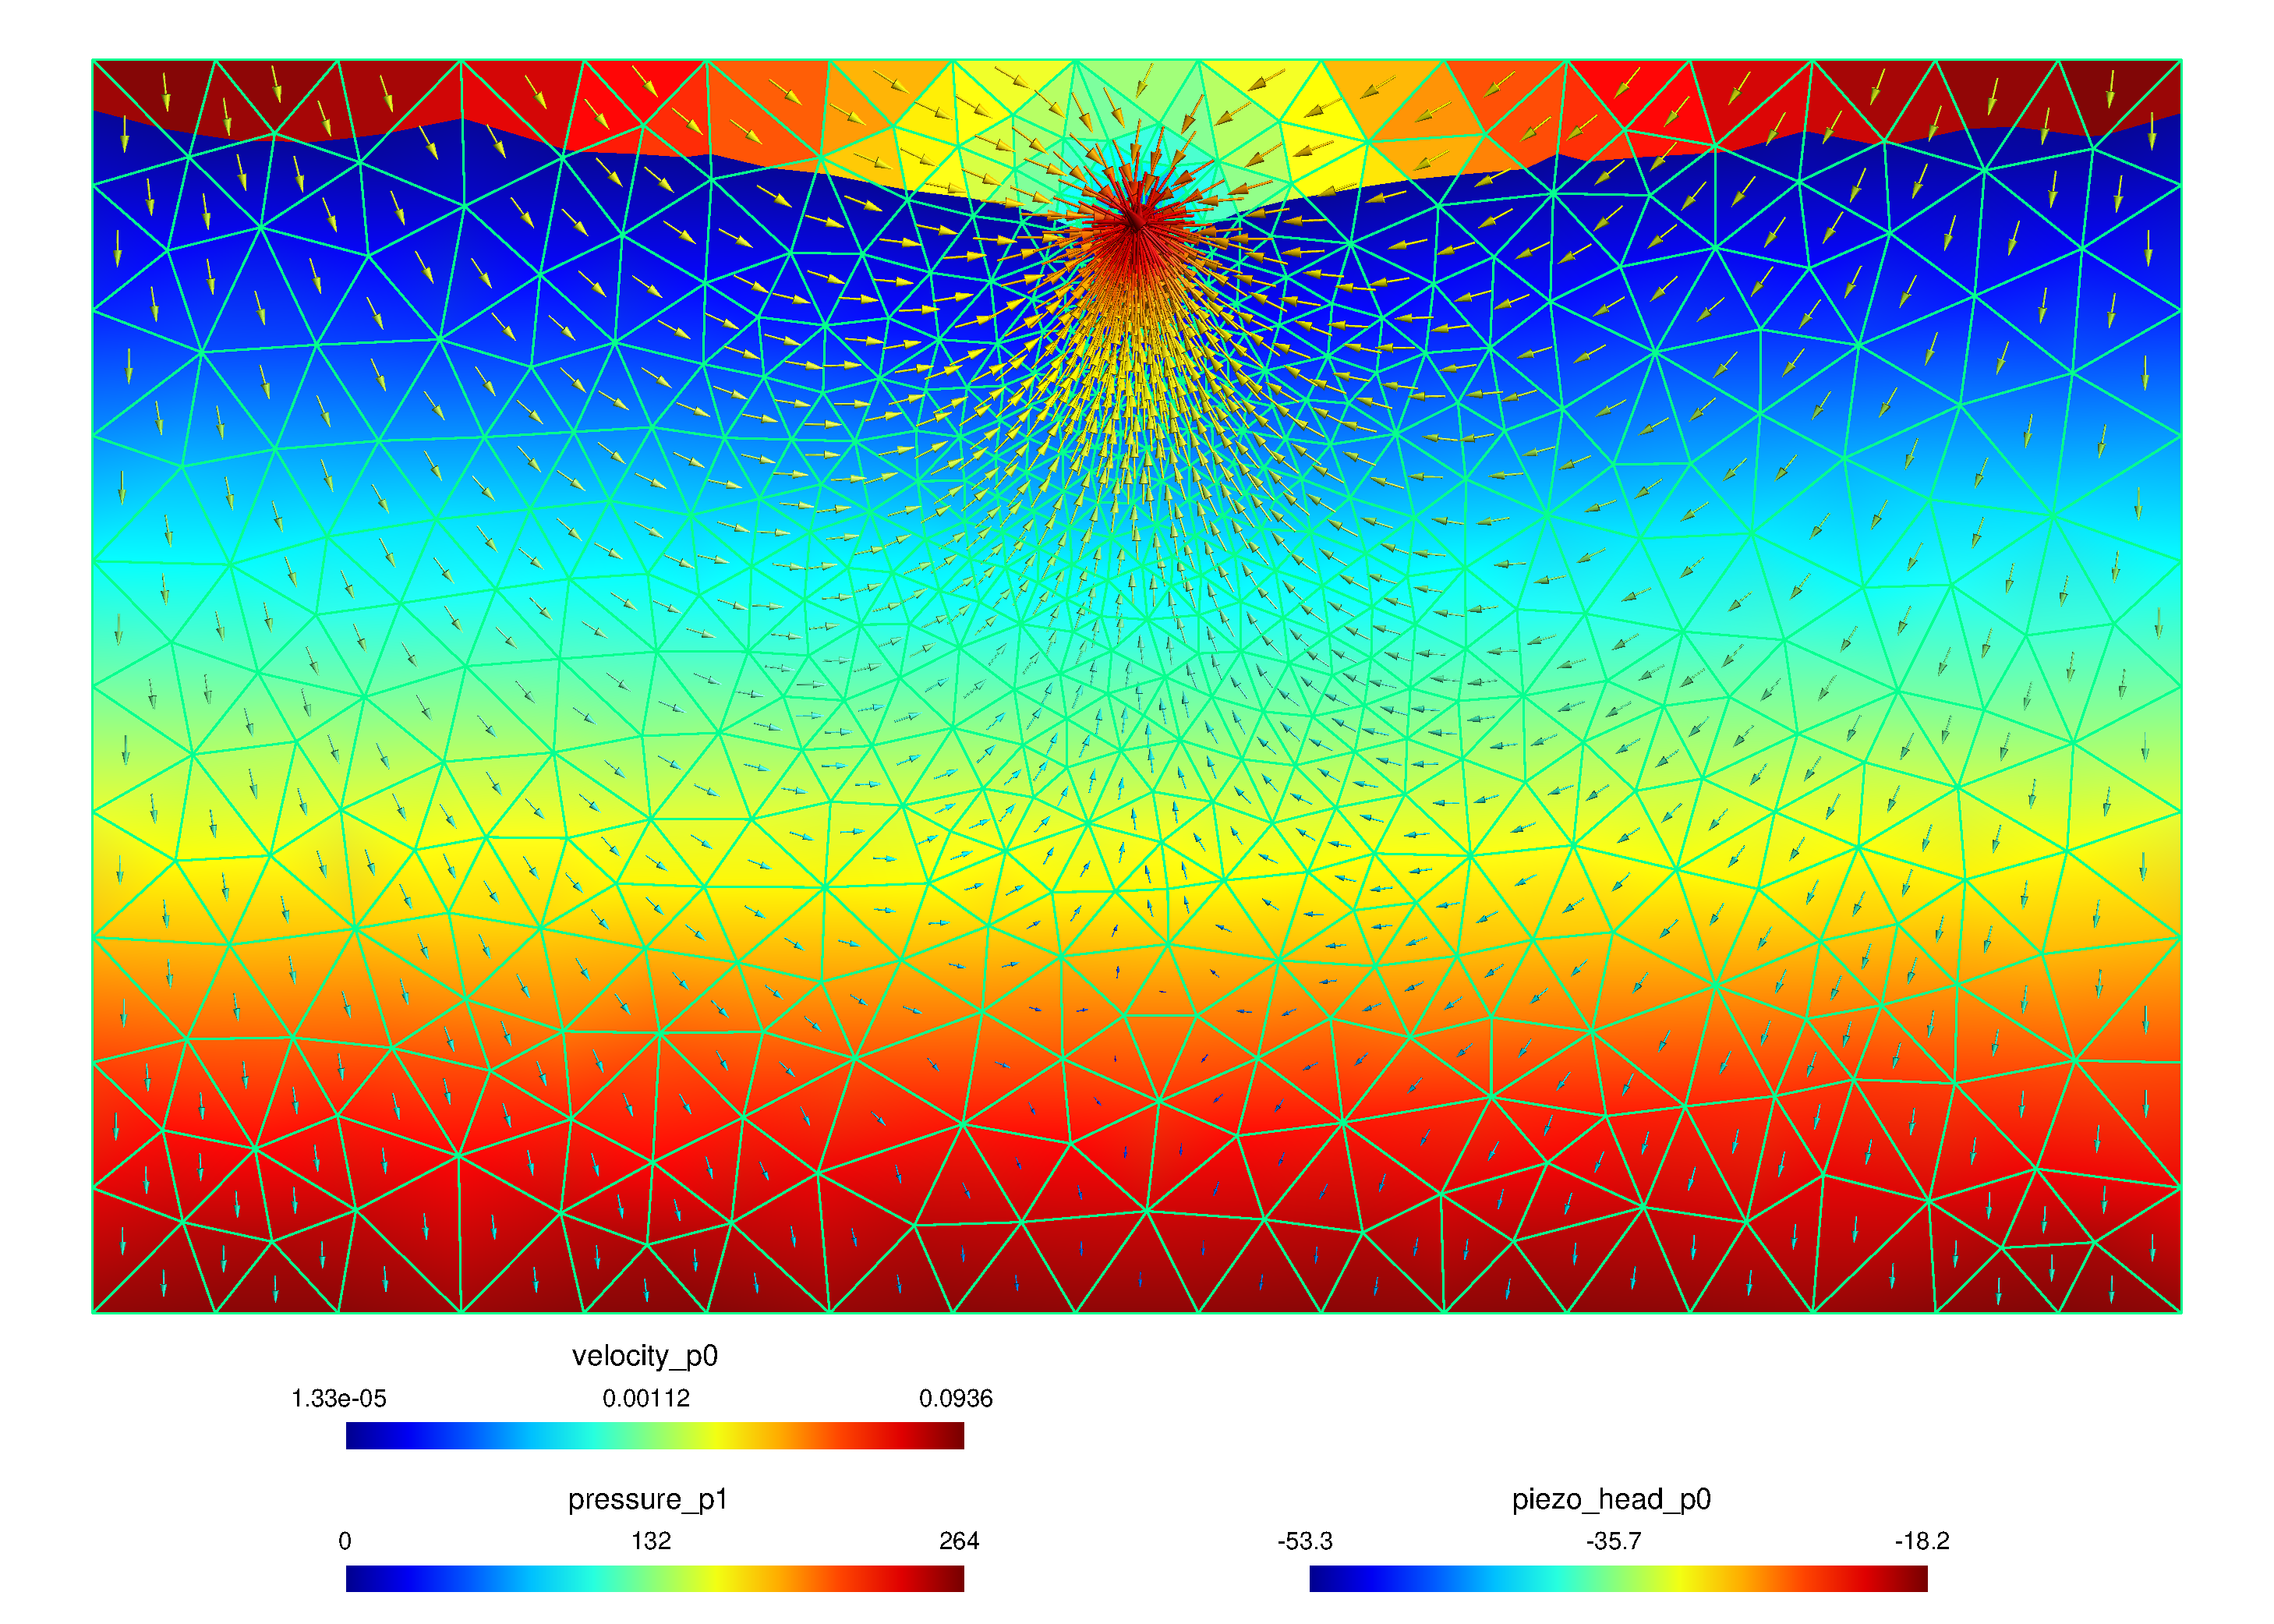
\includegraphics[scale=0.4]{\fig/03_flow.pdf}
        % 03_flow.pdf: 508x402 pixel, 72dpi, 17.92x14.18 cm, bb=0 0 508 402
        \caption{Elementwise pressure head and\\velocity field denoted by triangles.\\ (Steady flow.)}
        \label{fig:tut-flow}
    \end{subfigure}
    ~
    \begin{subfigure}[b]{0.45\textwidth}
        \centering
        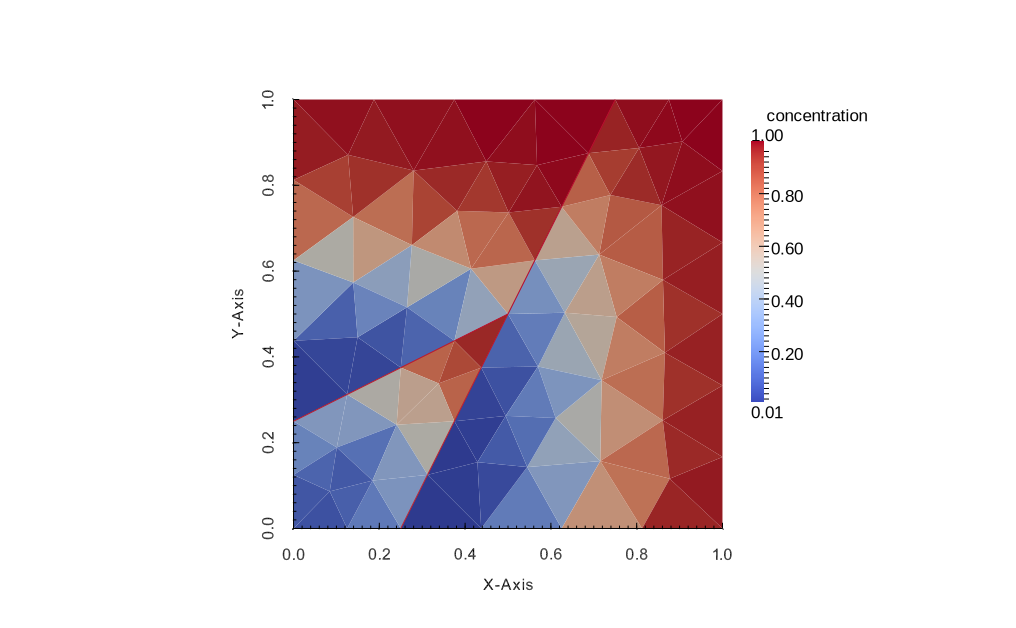
\includegraphics[scale=0.4]{\fig/03_trans.pdf}
        % 03_trans.pdf: 509x402 pixel, 72dpi, 17.96x14.18 cm, bb=0 0 509 402
        \caption{Propagation of U235 from the inflow part of the boundary. \\ (At the time 0.9 s.)}
        \label{fig:tut-trans}
    \end{subfigure}
    \caption{Results of the tutorial problem.}
    \label{fig:tutorial}
\end{figure}



% The output files can be either \verb'*.msh' files accepted by the GMSH or one can use VTK format that can be post-processed by Paraview.

In the following chapter we describe mathematical models used in Flow123d.
Then in chapter \ref{chapter:file-formats} we briefly describe structure of individual input files, in particular the main CON file.
The complete description of the CON format is given in chapter \ref{chapter:input-tree-reference}.


\chapter{Mathematical models \\of physical reality}
\label{PhysicalModels}

Flow123d provides models for Darcy flow in porous media as well as for the transport and reactions of solutes. In this section, we describe 
mathematical formulations of these models together with physical meaning and units of all involved quantities. In the first section we present 
basic notation and assumptions about computational domains and meshes that combine different dimensions. In the next section we
derive approximation of thin fractures by lower dimensional interfaces for a general transport process. Latter sections describe details for models of particular
physical processes.

\section{Meshes of mixed dimension}
Common and unique feature of all models in Flow123d is the support of
domains with mixed dimension. 
Let $\Omega_{3} \subset \Real^3$ be an open set representing continuous approximation of porous and fractured medium.
Similarly, we consider a 2D manifold $\Omega_2\subset\overline\Omega_3$, representing 2D fractures and a 1D manifold $\Omega_1\subset \overline\Omega_2$ of 1D channels or preferential paths (see Fig \ref{fig:multi-dim}).
We assume that $\Omega_2$ and $\Omega_1$ are polytopic (i.e. polygonal and piecewise linear, respectively).
For every dimension $d=1,2,3$, we introduce a triangulation $\mathcal{T}_{d}$ of the open set $\Omega_d$
that consists of finite elements $T_{d}^{i},$\ $i = 1,\dots,N_{E}^{d}$.
The elements are simplices, i.e. lines, triangles and tetrahedra, respectively.

\begin{figure}[h]
\centering
\includegraphics[width=10cm]{\fig/ground_fractures}
\caption{
    \label{fig:multi-dim}
    Scheme of a problem with domains of multiple dimensions.
}
\end{figure}

Present numerical methods require meshes satisfying the compatibility conditions
\begin{equation}
        T_{d-1}^i \cap T_d \subset \mathcal{F}_d,   \qquad \text{where } \mathcal{F}_d = \bigcup_{k} \partial T_{d}^{k}
\end{equation}
and
\begin{equation}
        T_{d-1}^i \cap \mathcal{F}_d    \text{ is either $T_{d-1}^i$ or $\emptyset$}    
\end{equation}
for every $i\in\{1,\dots, N_{E}^{d-1}\}$, $j\in\{1,\dots,N_{E}^{d}\}$,  and $d=2,3$. That is, the $(d-1)$-dimensional elements are either between $d$-dimensional elements and
match their sides or they poke out of $\Omega_d$. 

\section{Advection-diffusion processes on fractures}
\label{sc:ad_on_fractures}
In this section, we shall derive a model for a general advection-diffusion process in a domain of mixed dimensions using
simple approximations inspired by the paper \citet{martin_modeling_2005}. Let us consider a fracture as a strip domain 
\[
 \Omega_f \subset [0,\delta] \times \Real^{d-1}
\]
for $d=2$ or $d=3$ and surrounding continuum domains
\[
 \Omega_1 \subset (-\infty,0)\times \Real^{d-1},
 \Omega_2 \subset (\delta,\infty)\times \Real^{d-1}.
\]
Further, we denote by $\gamma_i$, $i=1,2$ the fracture faces common with domains $\Omega_1$ and $\Omega_2$ respectively.
By $x$, $\vc y$ we denote normal and tangential coordinate of a point in $\Omega_f$. 
We consider the normal vector  $\vc n=\vc n_1=-\vc n_2=(1,0,0)^\top$.
An advection-diffusion process is given by equations:
\begin{align}
  \label{eq:fr:continuity}
  \prtl_t w_i + \div \vc j_i &= f_i&&  \text{on } \Omega_i,\ i=1,2,f,\\
  \label{eq:fr:flux}
  \vc j_i &= - \tn A_i\grad u_i + \vc b_i w_i&& \text{on } \Omega_i,\ i=1,2,f,\\
  \label{eq:fr:Dirichlet}
  u_i &= u_f&& \text{on } \gamma_i,\ i=1,2,\\
  \label{eq:fr:Neumann}
  \vc j_i \cdot \vc n &= \vc j_f \cdot \vc n&& \text{on } \gamma_i,\ i=1,2,
\end{align}
where $w_i=w_i(u_i)$ is the conservative quantity and $u_i$ is the principal unknown, $\vc j_i$ is the flux of $w_i$, $f_i$ is the source term,
$\tn A_i$ is the diffusivity tensor and $\vc b_i$ is the velocity field. We assume that the tensor $\tn A_f$ is symmetric positive definite 
with one eigenvector in the direction $\vc n$. Consequently the tensor has the form:
\[
 A_f = \begin{pmatrix} 
            a_n & 0  \\
            0 & \tn A_t
       \end{pmatrix}
\]
Furthermore, we assume that $\tn A_f(x, \vc y)=\tn A_f(\vc y)$ is constant in the normal direction.

Our next aim is to integrate equations on the fracture $\Omega_f$ in the normal direction 
and obtain their approximations on the surface $\gamma=\Omega_f \cap \{x=\delta/2\}$ running through the middle of the fracture. 
For the sake of clarity, we will not write subscript $f$ for quantities on the fracture. 
To make the following procedure mathematicaly correct we have to assume that functions
$\prtl_x w$, $\prtl_x \grad_{\vc y} u$, $\prtl_x \vc b_{\vc y}$ are continuous and bounded on $\Omega_f$. Here and later on 
$\vc b_x=(\vc b \cdot \vc n)\, \vc n$ is the normal part of the velocity field and $\vc b_{\vc y} = \vc b - \vc b_x$ is the tangential part.
The same notation will be used for normal and tangential part of the field $\vc q$.

We integrate \eqref{eq:fr:continuity} over the fracture opening $[0,\delta]$ and use approximations to get
\begin{equation}
    \label{eq:fracture_continuity}
   \prtl_t (\delta W) - \vc j_2 \cdot \vc n_2 - \vc j_1 \cdot \vc n_1 + \div \vc J = \delta F,
\end{equation}
where for the first term, we have used mean value theorem, first order Taylor expansion, 
and boundedness of $\prtl_x w$ to obtain approximation:
\[
    \int_0^\delta w(x,\vc y) \d x=\delta w(\xi_{\vc y}, \vc y) = \delta W(\vc y) + O(\delta^2\abs{\prtl_x w}),
\]
where
\[
    W(\vc y)=w(\delta / 2,\vc y)=w(u(\delta/2,\vc y))=w(U(\vc y)).
\]
Next two terms in \eqref{eq:fracture_continuity} come from the exact integration 
of the divergence of the normal flux $\vc j_x$.
Integration of the divergence of the tangential flux $\vc j_{\vc y}$ gives the fourth term, where we introduced
\[
\vc J(\vc y) = \int_0^\delta \vc j_{\vc y}(x, \vc y) \d x.
\]
In fact, this flux on $\gamma$ is scalar for the case $d=2$. Finally, we integrate the right-hand side to get 
\[
    \int_0^\delta f(x,\vc y) \d x = \delta F(\vc y) + O(\delta^2\abs{\prtl_x f}),\quad F(\vc y)=f(\delta/2,\vc y). 
\]


Due to the particular form of the tensor $\tn A_f$, we can separately integrate tangential and normal
part of the flux given by \eqref{eq:fr:flux}. Integrating the tangential part and using approximations
\[
    \int_0^\delta  \grad_{\vc y} u(x, \vc y) \d x = \delta \grad_{\vc y} u (\xi_{\vc y}, \vc y) 
    = \delta \grad_{\vc y} U( \vc y) + O\big( \delta^2 \abs{\prtl_x\grad_{\vc y} u} \big) 
\]
and
\[
 \int_0^\delta \big(\vc b_{\vc y} w\big)(x, \vc y) \d x 
  = \delta \vc B(\vc y) W(\vc y) + O\big(\delta^2 \abs{\prtl_x(\vc b_{\vc y} w)} \big)
\]
where
\[
  \vc B(\vc y) = \vc b_{\vc y}(\delta/2, \vc y),
\]
we obtain
\begin{equation}
    \label{eq:fracture_darcy}
   \vc J = -\tn A_t \delta \grad_{\vc y} U + \delta \vc B W + O\big(\delta^2(\abs{\prtl_x\grad_{\vc y} u}+\abs{\prtl_x(\vc b_{\vc y} w)})\big).
\end{equation}


So far, we have derived equations for the state quantities $U$ and $\vc J$ on the fracture manifold $\gamma$. In order to
get a well possed problem, we have to prescribe two conditions for boundaries $\gamma_i$, $i=1,2$. To this end, we
perform integration of the normal flux $\vc j_x$, given by \eqref{eq:fr:flux}, separately for the left and right half of the fracture.
Similarly as before we use approximations
\[
 \int_0^{\delta/2} \vc j_x \d x = (\vc j_1 \cdot \vc n_1)\frac{\delta}{2} + O(\delta^2 \abs{\prtl_x \vc j_x})
\]
and 
\[
 \int_0^{\delta/2} \vc b_x w \d x = (\vc b_1 \cdot \vc n_1)\tilde{w}_1\frac{\delta}{2} + O(\delta^2 \abs{\prtl_x \vc b_x}\abs{w} + \delta^2\abs{\vc b_x}\abs{\prtl_x w})
\]
and their counter parts on the interval $(\delta/2, \delta)$ to get
\begin{align}
    \label{eq:fracture_normal_1}
     \vc j_1 \cdot \vc n_1 &= -\frac{2a_n}{\delta} (U - u_1) + \vc b_1\cdot \vc n_1 \tilde{w}_1\\
    \label{eq:fracture_normal_2}
    \vc j_2 \cdot \vc n_2 &= -\frac{2a_n}{\delta} (U - u_2) + \vc b_2\cdot \vc n_2 \tilde{w}_2
\end{align}
where $\tilde w_i$ can be any convex combination of $w_i$ and $W$. Equations \eqref{eq:fracture_normal_1}  
and \eqref{eq:fracture_normal_2} have meaning of a semi-discretized flux from domains $\Omega_i$ into fracture.
In order to get a stable numerical scheme, we introduce a kind of upwind already on this level using a different convex 
combination for each flow direction:
\begin{align}
   \notag 
   \vc j_i \cdot \vc n_i
       = &-\sigma_i (U - u_i)      \\ 
   \notag
      &+ \big[\vc b_i\cdot \vc n_i\big]^{+} \big(\xi w_i + (1-\xi) W\big)       \\
      \label{eq:fracture_normal}
      &+ \big[\vc b_i\cdot \vc n_i\big]^{-} \big((1-\xi) w_i + \xi W\big), \qquad i=1,2
\end{align}
where $\sigma_i = \frac{2a_n}{\delta}$ is the transition coefficient and the parameter $\xi\in [\frac12, 1]$ can be used to interpolate
between upwind ($\xi = 1$) and central difference ($\xi=\frac12$) scheme. Equations \eqref{eq:fracture_continuity}, \eqref{eq:fracture_darcy}, and
\eqref{eq:fracture_normal} describe the general form of the advection-diffusion process on the fracture and its communication with 
the surrounding continuum which we shall later apply to individual processes.




\section{Darcy Flow Model} \label{sec:darcy_flow}
We consider the simplest model for the velocity of the steady or unsteady flow in porous and fractured medium given by 
the Darcy flow:
\begin{equation}
    \label{eq:darcy}
    \vc w = -\tn K \grad H \quad\text{on }\Omega_d,\ \text{for $d=1,2,3$}.
\end{equation}
We drop the dimension index of quantities in equations if it is the same as the dimension of the set where the equation holds.
In \eqref{eq:darcy}, $\vc w_d$ \units{}{1}{-1} is \href{http://en.wikipedia.org/wiki/Superficial_velocity}{the superficial velocity},
$\tn K_d$ is the conductivity tensor, and $H_d$ \units{}{1}{} is the piezometric head. The velocity is related to the flux $\vc q_d$ 
\units{}{4-d}{-1} through
\[
    \vc q_d = \delta_d \vc w_d,
\]
where 
\hyperA{DarcyFlowMH-Data::cross-section}{$\delta_d$} 
\units{}{3-d}{} is a cross section coefficient, in particular $\delta_3=1$, $\delta_2$ \units{}{1}{} is the thickness of a fracture, and $\delta_1$ \units{}{2}{} is the cross-section of a channel.
The flux $\vc q_d\cdot\vc n$ is the volume of the liquid (water) that passes through a unit square ($d=3$),
unit line ($d=2$), or through a point ($d=1$) per one second. 
The conductivity tensor is given by the product \penalty-500
$\tn K_d = k_d \tn A_d$, where 
\hyperA{DarcyFlowMH-Data::conductivity}{$k_d>0$} is the hydraulic conductivity \units{}{1}{-1} and 
\hyperA{DarcyFlowMH-Data::anisotropy}{$\tn A_d$} is 
$3\times 3$ dimensionless anisotropy tensor which has to be symmetric and positive definite. The piezometric-head $H_d$ is related to the pressure head
$h_d$ by $H_d = h_d + z$ assuming that the gravity force acts in the negative direction of the $z$-axis. 
Combining these relations we get the Darcy law in the form:
\begin{equation}
    \label{eq:darcy_flux}
    \vc q = -\delta k\tn A \grad (h+z)  \qquad\text{in }\Omega_d,\ \text{for $d=1,2,3$}.
\end{equation}

Next, we employ the continuity equation for saturated porous medium and the dimensional reduction from the preceding section (with $w=u:=H$, $\vc j:=\vc w$, $\tn A:=\tn K$ and $\vc b:=\vc 0$), which yields:
\begin{equation}
    \label{eq:continuity}
    \prtl_t (\delta S\, h) + \div \vc q = F \qquad \text{in }\Omega_d,\ \text{for $d=1,2,3$},
\end{equation}
where \hyperA{DarcyFlowMH-Data::storativity}{$S_d$} \units{}{-1}{} is the storativity and $F_d$ \units{}{3-d}{-1} is a source term. In our setting the principal unknowns of the system 
(\ref{eq:darcy_flux}, \ref{eq:continuity}) are the pressure head $h_d$ and the flux $\vc q_d$.


The storativity (or the volumetric specific storage) $S_d>0$ can be expressed as
\begin{equation}
  S_d = \gamma_w(\beta_r + \vartheta \beta_w),
\end{equation}
where $\gamma_w$ \units{1}{-2}{-2} is the specific weight of water, $\vartheta$ \units{}{}{} is the porosity, $\beta_r$ is compressibility of the bulk material of the pores (rock)
and $\beta_w$ is compressibility of the water, both with units \units{-1}{1}{-2}. For steady problems we set $S_d=0$ for all dimensions $d=1,2,3$.
The source term $F_d$ on the right hand side of \eqref{eq:continuity} consists of the volume density of prescribed sources 
\hyperA{DarcyFlowMH-Data::water-source-density}{$f_d$} \units{}{}{-1} and flux from higher dimension. 
Exact formula is slightly different for every dimension and will be discussed presently.

In $\Omega_3$ we simply have $F_3  = f_3$ \units{}{}{-1}.

In the set $\Omega_2 \cap \Omega_3$ the fracture is surrounded by one 3D surface from every side (or just one surface since we allow also 2D models on the boundary).
On $\prtl\Omega_3 \cap \Omega_2$ we prescribe a boundary condition of Robin type:
\begin{align*}
        \vc{q}_3\cdot \vc n^{+} &= q_{32}^{+} =\sigma_{3} (h_3^{+}-h_2),\\
        \vc{q}_3\cdot \vc n^{-} &= q_{32}^{-} =\sigma_{3} (h_3^{-}-h_2),
\end{align*}
where $\vc{q}_3\cdot\vc n^{+/-}$ \units{}{1}{-1} is the outflow from $\Omega_3$, $h_3^{+/-}$ is
a trace of the pressure head in $\Omega_3$, $h_2$ is the pressure head in $\Omega_2$, and 
$\sigma_{3}$ \units{}{}{-1} is the transition coefficient given by (see section \ref{sc:ad_on_fractures} and \cite{martin_modeling_2005})
\[
\label{e:sigma3_law}
  \sigma_3 = \sigma_{32} \frac{2\tn K_2 :\vc n_2\otimes\vc n_2 }{\delta_2}.
\]
Here $\vc n_2$ is the unit normal to the fracture (sign doesn't matter).
On the other hand, the sum of the interchange fluxes $q_{32}^{+/-}$ forms
a volume source in $\Omega_2$.  Therefore $F_2$ \units{}{1}{-1} on the right hand side of \eqref{eq:continuity} is
given by
\begin{equation}
   \label{source_2D}
   F_2 = \delta_2 f_2 + (q_{32}^{+} + q_{32}^{-}).
\end{equation}

The communication between $\Omega_2$  and  $\Omega_1$ is similar.  However, in the 3D ambient space,
a 1D channel can join multiple 2D fractures $1,\dots, n$. Therefore, we have $n$
independent outflows from $\Omega_2$:
\begin{equation*}
        \vc{q}_2\cdot \vc n^{i} = q_{21}^{i} =\sigma_{2} (h_2^{i}-h_1),
\end{equation*}
where $\sigma_2$ \units{}{1}{-1} is the transition coefficient integrated over the width of the fracture $i$:
\[
\label{e:sigma2_law}
  \sigma_2 = \sigma_{21} \frac{2\delta_2^2\tn K_1:{\vc n_1^i}\otimes{\vc n_1^i}}{\delta_1}.
\]
Here $\vc n_1^i$ is the unit normal to the channel that is tangential to the fracture $i$.
Sum of the fluxes forms a part of $F_1$ \units{}{2}{-1}:
\begin{equation}
   \label{source_1D}
   F_1 = \delta_1 f_1 + \sum_{i=1}^n q_{21}^{i}. 
\end{equation}
We remark that the direct communication between 3D and 1D is neglected.
The transition coefficients 
\hyperA{DarcyFlowMH-Data::sigma}{$\sigma_{32}$} \units{}{}{} and
\hyperA{DarcyFlowMH-Data::sigma}{$\sigma_{21}$} \units{}{}{} are independent scaling parameters which represent the ratio of the crosswind and the tangential conductivity in the fracture.

In order to obtain unique solution we have to prescribe boundary conditions. Currently we support three basic 
\hyperA{DarcyFlowMH-Data::bc-type}{types of boundary conditions}. 
Consider a disjoint decomposition of the boundary
\[
    \prtl\Omega_d = \Gamma_d^D \cap \Gamma_d^N \cap \Gamma_d^R
\]
into Dirichlet, Neumann, and Robin parts. We prescribe
\begin{align}
    h_d &= h_d^D        &&\text{ on }\Gamma_d^D,\\
    \vc q_d \cdot \vc n &= q_d^N         &&\text{ on }\Gamma_d^N,\\
    \vc q_d \cdot \vc n &= \sigma_d^R ( h_d - h_d^R)     &&\text{ on }\Gamma_d^R.
\end{align}
where 
\hyperA{DarcyFlowMH-Data::bc-pressure}{$h_d^D$, $h_d^R$} 
is the given pressure head \units{}{1}{}, which alternatively can be prescribed through the piezometric head 
\hyperA{DarcyFlowMH-Data::bc-piezo-head}{$H_d^D$, $H_d^R$} 
respectively. 
\hyperA{DarcyFlowMH-Data::bc-flux}{$q_d^N$} 
is the given surface density of the boundary outflow \units{}{4-d}{-1}, and  
\hyperA{DarcyFlowMH-Data::bc-robin-sigma}{$\sigma_d^R$} 
is the transition coefficient \units{}{3-d}{-1}.
The problem is well posed only if there is Dirichlet or Robin boundary condition on every component of the set $\Omega_1 \cup \Omega_2 \cup \Omega_3$ and $\sigma_d >0$ for 
$d=2,3$.

For unsteady problems one has to specify an initial condition in terms of initial pressure head 
\hyperA{DarcyFlowMH-Data::init-pressure}{$h_d^0$} 
or initial piezometric head 
\hyperA{DarcyFlowMH-Data::init-piezo-head}{$H_d^0$}.

\paragraph{Volume balance.}
The equation \eqref{eq:continuity} satisfies the volume balance of the liquid in the following form:
\[ V(0) + \int_0^t s(\tau) \,d\tau - \int_0^t f(\tau) \,d\tau = V(t) \]
for any instant $t$ in the computational time interval.
Here
$$ V(t) := \sum_{d=1}^3\int_{\Omega^d}(\delta S h)(t,\vc x)\,d\vc x, $$
$$ s(t) := \sum_{d=1}^3\int_{\Omega^d}F(t,\vc x)\,d\vc x, $$
$$ f(t) := \sum_{d=1}^3\int_{\partial\Omega^d}\vc q(t,\vc x)\cdot\vc n(\vc x) \,d\vc x $$
is the volume \units{}{3}{}, the volume source \units{}{3}{-1} and the volume flux \units{}{3}{-1} of the liquid at time $t$, respectively.
The volume, flux and source on every geometrical region is calculated at each computational time step and the values together with the control sums are written to the file \texttt{water\_balance.txt}.






% ***************************************** SYMBOLS
\def\abs#1{\lvert#1\rvert}
\def\argdot{{\hspace{0.18em}\cdot\hspace{0.18em}}}
\def\avg#1{\left\{#1\right\}_\omega}
\def\D{{\tn D}}
\def\div{\operatorname{div}}
\def\Eh{\mathcal E_h}       % edges of \Th
\def\Ehcom{\mathcal E_{h,C}}         % edges of \Th on interface with lower dimension
\def\Ehdir{\mathcal E_{h,D}}         % Dirichlet edges of \Th
\def\Ehint{\mathcal E_{h,I}}       % interior edges of \Th
\def\grad{\nabla}
\def\jmp#1{[#1]}
\def\n{\vc n}
\def\vc#1{\mathbf{\boldsymbol{#1}}}     % vector
\def\R{\mathbb R}
\def\sc#1#2{\left(#1,#2\right)}
\def\Th{\mathcal T_h}       % triangulation
\def\th{\vartheta}
\def\tn#1{{\mathbb{#1}}}    % tensor
\def\Tr{\operatorname{Tr}}
\def\where{\,|\,}
%***************************************************************************


\section{Transport of substances}

Flow123d can simulate transport of substances dissolved in water.
The transport mechanism is governed by the \emph{advection}, and the \emph{hydrodynamic dispersion}.
Moreover the substances can move between ground and fractures.


In the domain $\Omega_d$ of dimension $d\in\{1,2,3\}$, we consider a system of mass balance equations in the following form:
\begin{equation}
    \label{e:ADE}
   \delta_d\partial_t ( \th c^i) + \div ( \vc q_d c^i ) - \div (\th \delta_d \D^i \grad c^i ) = F_S^i + F_C(c^i) + F_R(c^1,\dots, c^s).
\end{equation}
The principal unknown is the concentration $c^i$ \units{1}{-3}{} of a substance $i\in\{1,\dots, s\}$, which means weight of the substance in unit volume of the water.
Other quantities are:
\begin{itemize}

\item $\th$ \units{}{}{} is the \hyperA{TransportDG-BulkData::por-m}{porosity}, i.e. fraction of space occupied by water and the total volume.
\item The hydrodynamic dispersivity tensor $\D^i$ \units{}{2}{-1} has the form
\begin{equation} 
  \label{eqn:transport_disp}
  \D^i =D_m^i \tau \tn I + \abs{\vc v}\left(\alpha_T^i \tn I + (\alpha_L^i - \alpha_T^i) \frac{\vc v \times \vc v}{\abs{\vc v}^2}\right),
\end{equation}
which represents (isotropic) molecular diffusion, and mechanical dispersion in longitudal and transversal direction to the flow.
Here $D_m^i$ \units{}{2}{-1} is the \hyperA{TransportDG-BulkData::diff-m}{molecular diffusion coefficient} of the $i$-th substance (usual magnitude in clear water is $10^{-9}$), $\tau=\th^{1/3}$ is the tortuosity (by \cite{millington_quirk}), $\alpha_L^i$ \units{}{1}{} and $\alpha_T^i$ \units{}{1}{} is the \hyperA{TransportDG-BulkData::disp-l}{longitudal dispersivity} and the \hyperA{TransportDG-BulkData::disp-t}{transversal dispersivity}, respectively.
Finally, $\vc v$ \units{}{1}{-1} is the \emph{microscopic} water velocity, related to the Darcy flux $\vc q_d$ by the relation $\vc q_d = \th\delta_d\vc v$.
The value of $D_m^i$ for specific substances can be found in literature (see e.g. \cite{cislerova_vogel}).
For instructions on how to determine $\alpha_L^i$, $\alpha_T^i$ we refer to \cite{marsily,domenico_schwartz}.

\item $F_S^i$ \units{1}{-d}{-1} represents the density of concentration sources.
Its form is:
\begin{equation}
 F_S^i = \varrho^i_S + (c_S^i-c^i)\sigma_S. \label{eqn:transport_sources}
\end{equation}
Here $\varrho_S^i$ \units{1}{-d}{-1} is the \hyperA{TransportDG-BulkData::sources-density}{density of concentration sources}, $c_S^i$ is an \hyperA{TransportDG-BulkData::sources-conc}{equilibrium concentration} and $\sigma_S^i$ is the \hyperA{TransportDG-BulkData::sources-sigma}{concentration flux}.

\item $F_C(c^i)$ \units{1}{-d}{-1} is the density of concentration sources due to exchange between regions with different dimensions, see \eqref{e:FC} below.

\item The reaction term $F_R(\dots)$ \units{1}{-d}{-1} is currently neglected.
\end{itemize}



\paragraph{Initial and boundary conditions.}
At time $t=0$ the concentration is determined by the \hyperA{TransportDG-BulkData::init-conc}{initial condition}
$$ c^i(0,\vc x) = c^i_0(\vc x). $$
The physical boundary $\partial\Omega_d$ is decomposed into the parts $\Gamma_I\cup\Gamma_D\cup\Gamma_N\cup\Gamma_R$, which may change during simulation time.
The first part $\Gamma_I$ is further divided into two segments:
\begin{align*}
\Gamma_I^+(t) &= \{\vc x\in \partial\Omega_d\where \vc q(t,\vc x)\cdot\vc n(\vc x)<0\},\\
\Gamma_I^-(t) &= \{\vc x\in \partial\Omega_d\where \vc q(t,\vc x)\cdot\vc n(\vc x)\ge 0\},
\end{align*}
where $\vc n$ stands for the unit outward normal vector to $\partial\Omega_d$.
We prescribe the following boundary conditions:
On the inflow parts $\Gamma_I^+\cup\Gamma_D$, the user must provide \hyperA{TransportDG-BoundaryData::bc-conc}{Dirichlet boundary condition} $c_D^i$ for concentrations:
$$ c^i = c^i_D \mbox{ on }\Gamma_I^+\cup\Gamma_D. $$
On $\Gamma_I^-$ we impose homogeneous Neumann boundary condition:
$$ -\th\delta_d\D^i\nabla c^i\cdot\vc n = 0 \mbox{ on }\Gamma_I^-, $$
on $\Gamma_N$ we impose Neumann boundary condition with user-defined \hyperA{TransportDG-BoundaryData::bc-flux}{concentration flux} $f^i_N$:
$$ -\th\delta_d\D^i\nabla c^i\cdot\vc n = f^i_N \mbox{ on }\Gamma_N, $$
and finally on $\Gamma_R$ we impose Robin boundary condition through \hyperA{TransportDG-BoundaryData::bc-robin-sigma}{transition parameter} $\sigma^i_R$ and \hyperA{TransportDG-BoundaryData::bc-conc}{reference concentration} $c^i_D$:
$$ -\th\delta_d\D^i\nabla c^i\cdot\vc n = \sigma^i_R(c^i-c^i_D) \mbox{ on }\Gamma_R. $$






\paragraph{Communication between dimensions.}
Transport of substances is considered also on interfaces of physical domains with adjacent dimensions (i.e. 3D-2D and 2D-1D, but not 3D-1D).
Denoting $c_{d+1}$, $c_d$ the concentration of a given substance in $\Omega_{d+1}$ and $\Omega_d$, respectively, the comunication on the interface between $\Omega_{d+1}$ and $\Omega_d$ is described by:
\begin{equation}
  \label{e:inter_dim_flux}
  q^c = \delta_{d+1}\sigma^c (\th_{d+1} c_{d+1} - \th_d c_d) + \begin{cases}q^w c_{d+1} & \mbox{ if }q^w\ge 0,\\q^w c_d & \mbox{ if }q^w<0,\end{cases}
\end{equation}
where
\begin{itemize}
\item $q^c$ \units{1}{-d}{-1} is the density of concentration flux from $\Omega_{d+1}$ to $\Omega_d$,
\item $\sigma^c$ \units{}{1}{-1} is a \hyperA{TransportDG-BulkData::sigma-c}{transition parameter}.
Its nonzero value causes mass exchange between dimensions whenever the concentrations differ.
It is recommended to set either $\sigma^c=0$ (exchange due to water flux only) or, similarly as in \eqref{e:sigma_law},
\[
  \sigma^c \approx\frac{\delta_{d+1}}{\delta_d}\D:\n\otimes\n.
\]
\item $q^w$ \units{}{3-d}{-1} is the water flux from $\Omega_{d+1}$ to $\Omega_d$, i.e. $q^w = \vc q_{d+1}\cdot\n_{d+1}$.
\end{itemize}
Equation \eqref{e:inter_dim_flux} is incorporated as the total flux boundary condition for the problem on $\Omega_{d+1}$ and a source term in $\Omega_d$:
\begin{align}
-\th\delta_{d+1}\D\nabla c_{d+1}\cdot\vc n + q^w c_{d+1} &= q^c,\\
\label{e:FC}
F_C^d &= q^c.
\end{align}

\paragraph{Dual porosity.}
Up to now we have described the transport equation for the single porosity model. The dual porosity model splits the mass into to zones the mobile zone and the immbile zone. 
Both occupy the same macroscopic volume, however on the microscopic scale, the immobile zone is formed by the dead-end pores, where the liquid is traped and can not pass through.
The rest of the pore volume is ocuppied by the mobile zone. Since the liquid in the immobile pores is immobile, the exchange of the substance is only due to molecular diffusion.
We consider simple nonequilibrium linear model:
\begin{align}
    \theta_m \partial_t c_m &= \alpha ( c_i - c_m), \\
    \theta_i \partial_t c_i &= \alpha ( c_m - c_i) 
\end{align}
where $c_m$ is the concentration in the mobile zone, $c_i$ is the concentration in the immobile zone, $\alpha$ is a diffusion parameter, $\theta_m$ and $\theta_i$ are porosities of the mobile zone and the immobile zone respectively, while 
\[
  \theta_m +\theta_i =\theta.
\]

The solution of this system is:
\begin{align}
     c_m(t) &= (c_m(0) - c_a(0)) \exp(- \alpha(\frac{1}{\theta_m} + \frac{1}{\theta_i}) t) + c_a(0), \\
     c_i(t) &= (c_i(0) - c_a(0)) \exp(- \alpha(\frac{1}{\theta_m} + \frac{1}{\theta_i}) t) + c_a(0)
\end{align}
where $c_a$ is weighted average:
\[
  c_a = \frac{\theta_m c_m + \theta_i c_i}{\theta_m + \theta_i}.
\]


\paragraph{Mass balance.}
The advection-dispersion equation satisfies the balance of mass in the following form:
$$ m^i(0) + \int_0^t s^i(\tau) \,d\tau - \int_0^t f^i(\tau) \,d\tau = m^i(t) $$
for any instant $t$ in the computational time interval and any substance $i$.
Here
$$ m^i(t) := \sum_{d=1}^3\int_{\Omega^d}\delta_d\th c^i(t,\vc x)\,d\vc x, $$
$$ s^i(t) := \sum_{d=1}^3\int_{\Omega^d}F_S(t,\vc x)\,d\vc x, $$
$$ f^i(t) := \sum_{d=1}^3\int_{\partial\Omega^d}\left(\th\delta_d c^i(t,\vc x)\vc q(t,\vc x)\tn I - \th\delta_d\D^i\nabla c^i(t,\vc x)\right)\cdot\vc n \,d\vc x $$
is the mass \units{1}{}{}, the volume source \units{1}{}{-1} and the mass flux \units{1}{}{-1} of $i$-th substance at time $t$, respectively.
The mass, flux and source on every geometrical region is calculated at each computational time step and the values together with the control sums are written to the file \texttt{mass\_balance.txt}.







% ***************************************** SYMBOLS
\def\abs#1{\lvert#1\rvert}
\def\argdot{{\hspace{0.18em}\cdot\hspace{0.18em}}}
\def\avg#1{\left\{#1\right\}_\omega}
\def\D{{\tn D}}
\def\div{\operatorname{div}}
\def\Eh{\mathcal E_h}       % edges of \Th
\def\Ehcom{\mathcal E_{h,C}}         % edges of \Th on interface with lower dimension
\def\Ehdir{\mathcal E_{h,D}}         % Dirichlet edges of \Th
\def\Ehint{\mathcal E_{h,I}}       % interior edges of \Th
\def\grad{\nabla}
\def\jmp#1{[#1]}
\def\n{\vc n}
\def\vc#1{\mathbf{\boldsymbol{#1}}}     % vector
\def\R{\mathbb R}
\def\sc#1#2{\left(#1,#2\right)}
\def\Th{\mathcal T_h}       % triangulation
\def\th{\vartheta}
\def\tn#1{{\mathbb{#1}}}    % tensor
\def\Tr{\operatorname{Tr}}
\def\where{\,|\,}
%***************************************************************************

\section{Equilibrial Adsorption}\label{sec:sorp_math}
The simulation of monolayer, equilibrial adsorption is based on solution of the couple of equations representing mass balance law and empirical description of adsorption represented by comon types of isotherm. Considered types of isotherm folows:
\begin{itemize}
 \item Without adsorption, \hyperA{Sorption-BulkData::sorption-types}{$sorption\_type$} is $"none"$.
 \item Linear isotherm $c_s = f(c_a) = k_l\cdot c_a$, $sorption\_type$ is $"linear"$.
 \item Freundlichs' isotherm $c_s = f(c_a) = k_F\cdot c_a^{\alpha}$, $sorption\_type$ is $"freundlich"$.
 \item Langmuirs' isotherm $c_s = f(c_a) = k_L\cdot \frac{\alpha\cdot c_a}{1 + \alpha\cdot c_a}$, $sorption\_type$ is $"langmuir"$. Langmuirs isotherm has been derived form thermodynamic laws. $k_L$ denotes the maximal amount of sorbing specie which can be capt per unit volume of a bulk matrix. Coefficient $\alpha$ is a fraction of adsorption and desorption rate constant $\alpha = \frac{k_a}{k_d}$
\end{itemize}
Notification:
\begin{itemize}
 \item Sorbed concentration $[c_s] = \frac{[n]}{[m_H]} = \frac{N}{M} = \frac{Mol}{kg}$, where $m_H$ is the mass of bulk and $n$ denotes amount of substance in an element.
 \item Aqueous concentration $[c_a] = \frac{[m]}{[m_w]} = \frac{M}{M} = \frac{kg}{kg} = 1$, where $m_w$ is the mass of water/solvent in element. Just water ($\rho_w = 1~kg\cdot l^{-1}$) is supposed to be solvent in version 1.7.0. 
 \item Multiplication parameters, $k_i, ~i\in\{ l,F,L\}$, \hyperA{Sorption-BulkData::mult-coefs}{$mult\_coefs$} can have various physical dimensions.
 \item Aditional parameters, $[\alpha] = 1$, \hyperA{Sorption-BulkData::second-params}{$second\_params$}.
\end{itemize}
The mass balance equation can be derived from \ref{eq:mass_balance_base},
\begin{equation}
  m_{Total} = m_{aqueous} + m_{sorbed} = c_a\cdot V_{elm}\cdot\rho_w\cdot n + c_s\cdot M_s \cdot V_{elm}\cdot\rho_H\cdot(1-n)
  \label{eq:mass_balance_base}
\end{equation}
where $\rho_w$ denotes solvent density \hyperA{Sorptions::solvent-dens}{$solvent\_dens$}, $\rho_H$ is the symbol for \hyperA{Sorption-BulkData::rock-density}{$rock\_density$}, $V_{elm}$ denotes element volume, $n$ is the symbol for porosity, here, and $M_s$ denotes \hyperA{Sorptions::molar-masses}{$molar\_masses$}.

The equation \ref{eq:mass_balance_base} depends on volume of an element $V_{elm}$. We devide both sides by $V_{elm}$ to suppress this dependency and we get resulting mass balance equation \ref{eq:mass_balance_base2}.
\begin{equation}
 \begin{array}{l}
  konst._T = k_a\cdot c_a + k_s\cdot c_s\\
  k_a = \rho_w\cdot n\\
  k_s = M_s \cdot\rho_H\cdot(1-n)
 \end{array}
 \label{eq:mass_balance_base2}
\end{equation}

After the substitution $|c_s = f(c_a)|$ we become the equation, which can be either solved iteratively or aproximated through interpolation. This equation has following form.
\begin{equation}
 konst._T = k_a\cdot c_a + k_s\cdot f(c_a)
 \label{eq:nonlin_sorption}
\end{equation}
To solve the equation \ref{eq:nonlin_sorption} iteratively, it is very important to define interval where to look for solution (unknown $c_a$). The lower bound is $0$. Concentration can not reach negative values. The upper bound is derived using simple imagination. Lets suppose limmited \hyperA{Sorptions::solubility}{$solubility$} of selected transported substance and lets denote the limmit $c_a^{limmit}$. We keep the maximal "total mass" $konst._T^{limit}= k_a\cdot c_a^{limmit} + k_s\cdot f(c_a^{limmit})$, but we dissolve all the mass to get maximal $c_a^{max} > c_a^{limmit}$. That means $c_s = 0$ for this moment. To understand this step lets look at the figure \ref{fig:sorpce}. We can slightly enlarge the interval by setting the upper bound equal to $c_a^{max} + const_{small}$.

\begin{figure}[ht!]
 \centering
 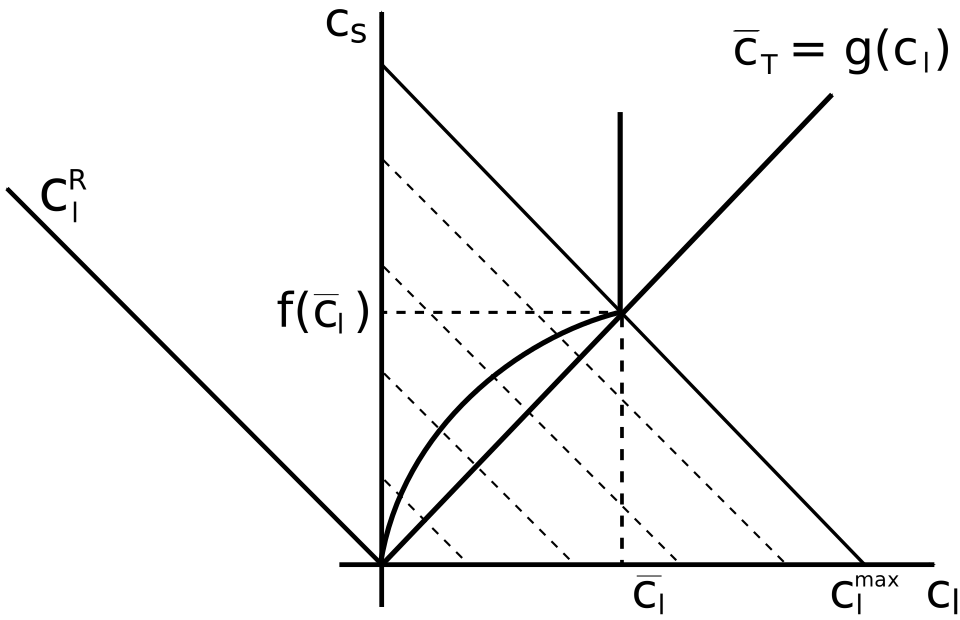
\includegraphics[scale = 1.0]{./sorpce}
 \caption{Sorption in combination with limmited solubility.}
 \label{fig:sorpce}
\end{figure}


To approximate the equation \ref{eq:nonlin_sorption} using interpolation we need to prepare the set of values which represent $[c_a, f(c_a)]$, with $c_a$ equidistantly distributed in transformed (rotated and rescaled) coordination system at first. The approach for construction of interpolation table follows.
\begin{enumerate}
 \item Maximal "total mass" $konst._T^{limit} = k_a\cdot c_a^{limmit} + k_s\cdot f(c_a^{limmit})$ is computed.
 \item Total mass step is derived $mass\_step = konst._T^{limit}/n\_steps$. $n\_steps$ is equal to \hyperA{Sorptions::substeps}{$substeps$} in con-file.
 \item Appropriate $c_a^i = (mass\_step\cdot i)/k_a,~i\in \{0,\ldots, n\_steps\}$ are computed. 
 \item The equations $k_a\cdot c_a^i = k_a\cdot c_a + k_s\cdot f(c_a)~i\in \{0,\ldots, n\_steps\}$ are solved for $c_a$ as unknown. The solution is the set of ordered couples (points) $[c_a^l,f(c_a^l)],~l\in\{0,\ldots,n\_steps\}$.
\end{enumerate}
After computation of $\{[c_a^l,f(c_a^l)]\}$ we transform these coordinates to the system where total mass is independent variable. This is done by multiplication of precomputed points using transformation matrix ${\bf A}$.
\begin{equation}
 \begin{array}{l}
  \overrightarrow{c}^R = {\bf A}\cdot\overrightarrow{c}\\
  \left[\begin{array}{c} c_a^{R,l}\\ c_s^{R,l} \end{array}\right] = 
  \left[\begin{array}{cc}
    n\cdot \rho_w & M_s(1 - n)\rho_H\\
    -M_s(1 - n)\rho_H & n\cdot \rho_w
  \end{array}\right]\cdot
  \left[\begin{array}{c} c_a^l\\ c_s^l \end{array}\right]\\
  l\in\{0,\ldots,n\_steps\}
 \end{array}
 \label{eq:transf_mat}
\end{equation}

The values $c_a^{R,l}$ are equidistantly distributed and there is no reason to save them, but the values $c_s^{R,l}$ are stored in onedimensional interpolation table.

Once we have the interpolation table, we can use it for projection of ${[c_a,c_s]}$ transport results on the isotherm under concideration. The approach look as folows.
\begin{enumerate}
 \item Achieved concentrations are transformed to the coordination system through multiplication with the matrix ${\bf A}$, see \ref{eq:transf_mat}.
 \item Transrformed values are interpolated.
 \item The result of interpolation is transformed back. The backward transformation consist of multiplication with ${\bf A}^T$ which is followed by rescaling the result. Rescaling the result is neccessery because  ${\bf A}$ is not orthonormal as it is shown bellow.
 \[
 \begin{array}{l}
 {\bf A}^T\cdot{\bf A} =
  \left((n - 1)^2\cdot M_s^2\cdot \rho_h^2 + n^2\cdot \rho_w^2\right)\cdot\left[\begin{array}{cc}
    1 & 0\\
    0 & 1
  \end{array}\right]
  \end{array}
 \]
\end{enumerate}


\subsection{Limmited Solubility}\label{subsec:lim_solub}
When $k_a\cdot c_a + k_s\cdot f(c_a) > k_a\cdot c_a^{limmit} + k_s\cdot f(c_a^{limmit})$ neither iterative solver nor interpolation table is used. The aqueous concentration is set to be $c_a^{limmit}$ and sorbed concentration is computed $c_s = (k_a\cdot c_a + k_s\cdot f(c_a) - k_a\cdot c_a^{limmit})/k_s$.

% TODO: Describe reactions, decays, numerical methods
%% Copyright (C) 2007 Technical University of Liberec.  All rights reserved.
%
% Please make a following refer to Flow123d on your project site if you use the program for any purpose,
% especially for academic research:
% Flow123d, Research Centre: Advanced Remedial Technologies, Technical University of Liberec, Czech Republic
%
% This program is free software; you can redistribute it and/or modify it under the terms
% of the GNU General Public License version 3 as published by the Free Software Foundation.
%
% This program is distributed in the hope that it will be useful, but WITHOUT ANY WARRANTY;
% without even the implied warranty of MERCHANTABILITY or FITNESS FOR A PARTICULAR PURPOSE.
% See the GNU General Public License for more details.
%
% You should have received a copy of the GNU General Public License along with this program; if not,
% write to the Free Software Foundation, Inc., 59 Temple Place - Suite 330, Boston, MA 021110-1307, USA.

\normalsize

\subsection{Linear reactions}
\label{sec:linear_reactions}
The software suppports linear chemical reactions in the transport operator splitting method. 
The linear chemical reactions (we will recall them only as 'reactions' in this section) can desribe
\begin{itemize}
  \item first order kinetic chemical reactions
  \item radioactive decays, their chains and also complex chains with branches.
\end{itemize}
In the first case, the kinetics of a reaction is determined by a kinetic constant \hyperA{Substep::kinetic}{$k$}. 
In the second case, the radioactive decay is determined by the half life of the reactant 
\hyperA{Substep::half-life}{$t_{1/2}$}. Both notations
%
\[ A\xrightarrow{k} B, \qquad A\xrightarrow{t_{1/2}} B \]
%
express the same reaction and are governed by the same first order differential equation 
%
\[ \frac{\d c_A}{\d\tau} = -kc_A = - \frac{\ln 2}{t_{1/2}}\, c_A. \]
%
The relation between $k$ and $t_{1/2}$ is derived below
\begin{eqnarray*}
    \frac{\d c_A}{\d\tau} &=& -k c_A\\
    \frac{\d c_A}{c_A} &=& -k \d\tau\\
    \int\limits_{c_A^0}^{c_A^0/2}\frac{\d c_A}{c_A} &=& -k\int\limits_{0}^{t_{1/2}} 1\d\tau\\
    \big[ \ln c_A\big]^{c_A^0/2}_{c_A^0} &=& -\big[k\tau\big]^{t_{1/2}}_{0}\\
    \ln\frac{c_A^0}{2} - \ln c_A^0 &=& - k t_{1/2}\\
    \ln 2 &=& k t_{1/2}\\
    k &=& \frac{\ln 2}{t_{1/2}}.
\end{eqnarray*}



Lets consider to have a narrow decay chain without branches. This kind of decay chain can be described by following equation
\[
 A\xrightarrow{t_{1/2,A}}B\xrightarrow{t_{1/2,B}}C\xrightarrow{t_{1/2,C}}D\xrightarrow{t_{1/2,D}}E,
\]
where letters $\{A,\ldots, E\}$ denotes isotopes contained in considered decay chain and ${t_{1/2},i},~i\in\{A,\ldots, E\}$ is a symbol for a half-life of $i$-th isotope.
For a simulation of radioactive decay and first order reactions matrix multiplication based approach has been developed. It has been based on an arrangement of all the data to matrices. The matrix ${\bf C}^k$ contains the information about concentrations of all species ($s$) in all observed elements ($e$). The upper index $k$ denotes $k$-th time step. The matrix ${\bf C}^k$ has the dimension $e\times s~( rows \times columns)$.
The transport simulation is realized by matrix multiplication 
\[
  {\bf T}\cdot{\bf C}^k = {\bf C}^{k+1},
\]
where ${\bf T}$ is a square, block-diagonal matrix, representing a set of algebraic equations constructed from a set of partial differential equations.
When the simulation of the radioactive decay or the first order reaction is switched on, one step of
simulation changes to 
\[
  {\bf T}\cdot{\bf C}^k\cdot{\bf R} = {\bf C}^{k+1},
\]
where ${\bf R}$ is a square matrix with the dimension $(s \times s)$ . It is much easier to construct and to use ${\bf R}$ , than to include chemical influence to the transport
matrix ${\bf T}$ , because the matrix ${\bf R}$ has usually a simple structure and $s$ is much smaller than $e$. In the most simple case, when the order of identification numbers of isotopes in considered decay chain is the same as the order of identifiers of species transported by groundwater, then just two
diagonals are engaged and the matrix R looks as follows:

\begin{tiny}\[
   \begin{array}{l}
    {\bf R} = \left(
    \begin{array}{cccccc}
     \left(\frac{1}{2}\right)^\frac{\Delta t}{t_{1/2,1}} & 1 - \left(\frac{1}{2}\right)^\frac{\Delta t}{t_{1/2,i}} & 0 & \hdots & \hdots & 0\\
     0 & \left(\frac{1}{2}\right)^\frac{\Delta t}{t_{1/2,2}} & 1 - \left(\frac{1}{2}\right)^\frac{\Delta t}{t_{1/2,2}} & 0 & \ddots & 0 \\
     \vdots & \ddots & \ddots & \ddots & \ddots & \vdots\\
     0 & \ddots & 0 & \left(\frac{1}{2}\right)^\frac{\Delta t}{t_{1/2,n-2}} & 1 - \left(\frac{1}{2}\right)^\frac{\Delta t}{t_{1/2,n-2}} & 0 \\
     0 & \hdots & \hdots & 0 & \left(\frac{1}{2}\right)^\frac{\Delta t}{t_{1/2,n-1}} & 1 - \left(\frac{1}{2}\right)^\frac{\Delta t}{t_{1/2,n-1}}\\
     0 & \hdots & \hdots & 0 & 0 & 1
    \end{array}\right)
   \end{array}
\]\end{tiny}

Every single $j$-th column, except the first one, includes the contribution $1 - \left(\frac{1}{2}\right)^\frac{\Delta t}{t_{1/2,j}},~j\in\{A,\ldots, E\}$ from $(j-1)$-th
isotope with its half-life $t_{1/2,j-1}$. The term $\left(\frac{1}{2}\right)^\frac{\Delta t}{t_{1/2,j}}$ describes concentration decrease caused by the radioactive decay of $j$-th isotope itself. In general cases the matrix ${\bf R}$ can have much more complicated structure, especially when the considered decay chain has more branches.
The implementation of the radioactive decay in Flow123D does not firmly include standard natural decay chain. Instead of that it is possible for a user to define his/her decay chain.

It is also possible to simulate decay chains with branches as picture \ref{pic:dec_branches} shows.

\begin{figure}[htb]
 \centering
 \includegraphics[width = 8cm]{\fig /decay_chain.png}
 \caption{Decay chain with branches.}
 \label{pic:dec_branches}
\end{figure}


When it comes to a simulation of first order reactions, the kinetic constant is given as an input. 
The description of a kinetic chemical reaction has obviously two folowing forms
\[
  \begin{array}{l}
    A\xrightarrow{k}B,\\
    \frac{dc^A}{dt} = -k \cdot c^A.
  \end{array}
\]
The first one description is a standard chemical one. The second equation describes temporal decrease in amount of concentrations of the specie $c^A$. The constant $k$ is so called kinetic constant and for the case of a first order reactions it is equal to so called reaction rate. The order of reaction with just one reactant is equal to the power of $c^A$ in partial diferential reaction.

For an inclusion of first order reaction into a reaction matrix a half-life needs to be computed from the corresponding kinetic constant $k$. The derivation follows
\[
  \begin{array}{l}
    A\xrightarrow{k} B\\
    \frac{dc^A}{d\tau} = -k\cdot c_A\\
    \frac{dc^A}{c^A} = -k\cdot d\tau\\
    \int\limits_{c^A_0/2}^{c^A_0}\frac{dc^A}{c^A} = -k\cdot\int\limits_{t_{1/2,A}}^{0} d\tau\\
    \left[ ln c^A\right]_{c^A_0/2}^{c^A_0} = -[k\tau]_{t_{1/2,A}}^{0}\\
    ln c^A_0 - \ln\frac{c^A_0}{2} = k\cdot t_{1/2,A}\\
%     c^A (t) = c^A_0\cdot e^{-k\cdot t_{1/2,A}}\\
%     {\bf substitution} \qquad c^A(t_{1/2,A}) = \frac{1}{2}\cdot c^A_0\\
%     \frac{1}{2} c^A_0 = c^A_0\cdot e^{-k_1\cdot t_{1/2,A}}\\
    \ln 2 = k \cdot t_{1/2,A}\\
    t_{1/2,A} = \frac{ln 2}{k}
  \end{array}                                                                                                                                                                                                                                                                                                            
\]
The matrix ${\bf R}$ is constructed in the same way as for the radioactive
decay.


\section{Heat Transfer}
\label{sc:heat}

Under the assumption of thermal equilibrium between the solid and liquid phase, the energy balance equation has the form\footnote{For lower dimensions this form can be derived as in Section \ref{sc:ad_on_fractures} using $w:=\delta\tilde s T$, $u:=T$, $\tn A:=\delta\lambda\tn I$, $\vc b:=\frac{\varrho_l c_l}{\tilde s}\vc w$.}
\[
    \partial_t\left(\delta \tilde s T \right) + \div(\varrho_l c_l T \vc q) - \div(\delta\Lambda\nabla T) = F^T + F^T_C.
\]
The principal unknown is the temperature $T$ [K].
Other quantities are:
\begin{itemize}
\item \hyperA{HeatTransfer-DG-Data::fluid-density}{$\varrho_l$}, \hyperA{HeatTransfer-DG-Data::solid-density}{$\varrho_s$} \units{1}{-3}{} is the density of the fluid and solid phase, respectively.
\item \hyperA{HeatTransfer-DG-Data::fluid-heat-capacity}{$c_l$}, \hyperA{HeatTransfer-DG-Data::solid-heat-capacity}{$c_s$} [J$\mathrm{kg}^{-1}\mathrm{K}^{-1}$] is the heat capacity of the fluid and solid phase, respectively.
\item $\tilde s$ [J$\mathrm{m}^{-3}\mathrm{K}^{-1}$] is the volumetric heat capacity of the porous medium defined as
\[ \tilde s = \hyperA{HeatTransfer-DG-Data::porosity}{\th}\varrho_l c_l + (1-\th)\varrho_s c_s. \]
\item $\Lambda$ [W$\mathrm{m}^{-1}\mathrm{K}^{-1}$] is the thermal dispersion tensor:
\[ \Lambda = \Lambda^{cond} + \Lambda^{disp} \]
\[ \Lambda^{cond} = \left(\th \lambda_l^{cond} + (1-\th)\lambda_s^{cond}\right)\tn I, \]
\[ \Lambda^{disp} = \th \varrho_l c_l|\vc v|\left(\alpha_T\tn I + (\alpha_L-\alpha_T)\frac{\vc v\otimes\vc v}{|\vc v|^2}\right), \]
where \hyperA{HeatTransfer-DG-Data::fluid-heat-conductivity}{$\lambda_l^{cond}$}, \hyperA{HeatTransfer-DG-Data::solid-heat-conductivity}{$\lambda_s^{cond}$} [W$\mathrm{m}^{-1}\mathrm{K}^{-1}$] is the thermal conductivity of the fluid and solid phase, respectively, and \hyperA{HeatTransfer-DG-Data::disp-l}{$\alpha_L$}, \hyperA{HeatTransfer-DG-Data::disp-t}{$\alpha_T$} \units{}{1}{} is the longitudal and transverse dispersivity in the fluid.

\item $F^T$ [J$\mathrm{m}^{-d}\mathrm{s}^{-1}$] represents the thermal source:
\[ F^T = \delta \th F^T_l + \delta (1-\th) F^T_s, \]
\[ F^T_l = f_l^T + \varrho_l c_l \sigma^T_l(T-T_l), \]
\[ F^T_s = f_s^T + \varrho_s c_s \sigma^T_s(T-T_s), \]
where \hyperA{HeatTransfer-DG-Data::fluid-thermal-source}{$f_l^T$}, \hyperA{HeatTransfer-DG-Data::solid-thermal-source}{$f_s^T$} [W$\mathrm{m}^{-3}$] is the density of thermal sources in fluid and solid, respectively, \hyperA{HeatTransfer-DG-Data::fluid-ref-temperature}{$T_l$}, \hyperA{HeatTransfer-DG-Data::solid-ref-temperature}{$T_s$} [K] is a reference temperature and \hyperA{HeatTransfer-DG-Data::fluid-heat-exchange-rate}{$\sigma^T_l$}, \hyperA{HeatTransfer-DG-Data::solid-heat-exchange-rate}{$\sigma^T_s$} \units{}{}{-1} is the heat exchange rate.
\end{itemize}



\paragraph{Initial and boundary conditions.}
At time $t=0$ the temperature is determined by the \hyperA{HeatTransfer-DG-Data::init-temperature}{initial condition} $T_0$ [K]:
\[ T(0,\vc x) = T_0(\vc x). \]
Given the decomposition of $\partial\Omega_d$ into $\Gamma_I\cup\Gamma_D\cup\Gamma_{TF}\cup\Gamma_{DF}$ (see also Section \ref{sc:transport_model}), we prescribe the following boundary conditions:
\begin{itemize}
\item \textbf{inflow} Default boundary condition. On the inflow $\Gamma_I^+$ the \hyperA{HeatTransfer-DG-Data::bc-temperature}{reference temperature} $T_D$ [K] is enforced through total flux:
\[ \left(\varrho_l c_l T \vc q - \delta\Lambda\nabla T\right)\cdot\vc n = \varrho_l c_l T_D\vc q\cdot\vc n, \]
while on the outflow $\Gamma_I^-$ we prescribe zero diffusive flux:
\[ -\delta\Lambda\nabla T\cdot\vc n = 0. \] 
\item \textbf{dirichlet} On $\Gamma_D$, the Dirichlet condition is imposed via \hyperA{HeatTransfer-DG-Data::bc-temperature}{prescribed temperature} $T_D$:
\[ T = T_D \mbox{ on }\Gamma_I^+\cup\Gamma_D. \]
\item \textbf{total\_flux}
On $\Gamma_{TF}$ we impose total energy flux condition:
\[ \left(\varrho_l c_l T \vc q - \delta\Lambda\nabla T\right)\cdot\vc n = \delta(f^T_N+\sigma^T_R(T-T_D)). \]
with user-defined \hyperA{HeatTransfer-DG-Data::bc-flux}{energy flux} $f^T_N$ [J$\mathrm{m}^{-2}\mathrm{s}^{-1}$],
\hyperA{HeatTransfer-DG-Data::bc-robin-sigma}{transition parameter} $\sigma^T_R$ [J$\mathrm{m}^{-2}\mathrm{s}^{-1}\mathrm{K}^{-1}$] and \hyperA{HeatTransfer-DG-Data::bc-temperature}{reference temperature} $T_D$.
\item \textbf{diffusive\_flux} Finally on $\Gamma_{DF}$ we prescribe diffusive energy flux (similarly as above):
\[ -\delta\Lambda\nabla T\cdot\vc n = \delta(f^T_N+\sigma^T_R(T-T_D)). \]
\end{itemize}
We mention several typical uses of boundary conditions:
\begin{itemize}
\item natural inflow: Use dirichlet or inflow b.c. (the later type is useful when the location of liquid inflow is not known a priori) and specify $T_D$.
\item natural outflow: The energy in the domain decreases only due to advection. Use zero diffusive\_flux or inflow (the latter in case that the outflow boundary is not known a priori).
\item boundary with known energy flux: Use total\_flux and $f_N^T$.
\item thermally insulated boundary: Use zero total\_flux.
\item partially permeable boundary: The energy transfer is proportional to the temperature difference inside and outside the domain.
Use diffusive\_flux, $T_D$ and $\sigma_R^T$.
\end{itemize}






\paragraph{Communication between dimensions.}
Denoting $T_{d+1}$, $T_d$ the temperature in $\Omega_{d+1}$ and $\Omega_d$, respectively, the communication on the interface between $\Omega_{d+1}$ and $\Omega_d$ is described by the quantity
\begin{equation}
  \label{e:inter_dim_flux_heat}
  q^T_{d+1,d} = \sigma^T_{d+1,d} \frac{\delta_{d+1}^2}{\delta_d}2\Lambda_d:\n\otimes\n ( T_{d+1} - T_d) + \begin{cases} \varrho_l c_l q^l_{d+1,d} T_{d+1} & \mbox{ if }q^l_{d+1,d}\ge 0,\\\varrho_l c_l q^l_{d+1,d} \frac{\tilde s_d}{\tilde s_{d+1}} T_d & \mbox{ if } q^l_{d+1,d}<0,\end{cases}
\end{equation}
where
\begin{itemize}
\item $q^T_{d+1,d}$ [W$\mathrm{m}^{-2}$] is the density of heat flux from $\Omega_{d+1}$ to $\Omega_d$,
\item \hyperA{HeatTransfer-DG-Data::fracture-sigma}{$\sigma^T_{d+1,d}$} \units{}{}{} is a transition parameter.
Its value determines the exchange of energy between dimensions due to temperature difference.
In general, it is recommended to leave the default value $\sigma^T=1$ or to set $\sigma^T=0$ (when exchange is due to water flux only).
\item $q^l_{d+1,d}=\vc q_{d+1}\cdot\vc n$ is the water flux from $\Omega_{d+1}$ to $\Omega_d$.
\end{itemize}
The communication between dimensions is incorporated as the total flux boundary condition for the problem on $\Omega_{d+1}$:
\begin{equation}
\label{e:heat_FC}
\left(\varrho_l c_l T \vc q - \delta\Lambda\nabla T\right)\cdot\vc n = q^T
\end{equation}
and a source term in $\Omega_d$:
\begin{equation}
F^T_{C3} = 0,\quad
F^T_{C2} = q^T_{32},\quad
F^T_{C1} = q^T_{21}.
\end{equation}




\paragraph{Energy balance.}
The heat equation satisfies the balance of energy in the following form:
$$ e(0) + \int_0^t s(\tau) \,d\tau - \int_0^t f(\tau) \,d\tau = e(t) $$
for any instant $t$ in the computational time interval.
Here
$$ e(t) := \sum_{d=1}^3\int_{\Omega^d}(\delta \tilde s T)(t,\vc x)\,d\vc x, $$
$$ s(t) := \sum_{d=1}^3\int_{\Omega^d}F_S^T(t,\vc x)\,d\vc x, $$
$$ f(t) := \sum_{d=1}^3\int_{\partial\Omega^d}\left(\varrho_l c_l T\vc q - \delta\Lambda\nabla T\right)(t,\vc x)\cdot\vc n \,d\vc x $$
is the energy [J], the volume source [J$\mathrm{s}^{-1}$] and the energy flux [J$\mathrm{s}^{-1}$] at time $t$, respectively.
The energy, flux and source on every geometrical region is calculated at each computational time step and the values together with the control sums are written to the file \texttt{energy\_balance.txt}.







% TODO: Update numerical topics
% \input{numerical}



%\subsection{General Chemical Reactions}
For a simulation of general chemical reactions as a part of reactive transport simulation, an application Semchem has been merged together with Flow123D. It enables to simulate following types of reactions:
\begin{itemize}
  \item Chemical equilibrium (solved using iterative Newtons method)
    \subitem mathematical description $K^{(r)} = \prod_i c_i^{\alpha_i^{(r)}},$

  \item Slow evolving chemical kinetics (solved using Runge-Kutta method)
    \subitem mathematical description $\frac{dc_i}{dt} = -k^{(r)}\prod_j c_j^{\beta_j^{(r)}},$

  \item Fast evolving chemical kinetics (discretized using implicit Eulerova method and solved using Newtons method)
     \subitem mathematical description $\frac{c_i^{(T+1)} - c_i^{T}}{\Delta t} = -k^{(r)}\prod_j c_j^{\beta_j^{(r),(T+1)}},$
  \item Radioactive decay can be simulated as a special case of first order reaction.
\end{itemize}

Further informations can be found in ``Snizeni poctu nelinearnich rovnic popisujicich chemicke reakce''.


\chapter{File formats}
\label{chapter:file-formats}
%\section{Input format}

In this chapter, we shall describe structure of the main input file and data formats of other input files.
In particular we briefly describe the GMSH file format used for both the computational mesh as well as for the input of general spatial data.


\section{Main Input File}
\label{sec:CONformat}

In this section, we shall describe structure of the main input file that is given either as the first positional argument or through 
the parameter \verb'-s' on the command line. First, we provide a quick introduction to the YAML file format. Then, we demonstrate the most important 
input structures on the examples. 







\subsection{YAML basics}
YAML is a human readable data format. It is designed to be both human readable and human editable. As it is not a markup languages, there are
no tags to determine type of the data. The indentation and justification is used instead for data organization. Moreover the used YAML format (version 1.2) is 
superset of the JSON format, another minimalist data serialization format where braces and brackets are used instead of indentation.
For the more detailed description see \href{https://en.wikipedia.org/wiki/YAML}{Wikipedia} 
for further technical details and for reference parsers for various programming languages see YAML \href{http://yaml.org/}{home page} .

\subsubsection{Hierarchy of Mappings and Lists}
Elementary data are organized to lists and mappings. Let us start with an example of a list:
\begin{verbatim}
# Example of list 
- 3.14                  # a number
- 2014-01-14            # a date
- Simple string.        # a string
- "3 is three"          # quoting necessary
- '3 is three'          # other qouting
- true                  # boolean
\end{verbatim}
Comments are started by a hash (\verb'#') which can appear anywhere on a line and marks the comment up to the end of line.
The the list follows with singel item per line preceded by a dash (\verb'-'). Any value starting by a digit is interpreted as a number
or date. Values starting with letter is interpreted as a string. Otherwise one may use double (\verb'""') or single (\verb"''") 
quotas to mark a string value explicitly. Finally some strings are interpreted as boolean values, it is recommended to use 
\verb'true' and \verb'false' (other possible pairs are e.g. \verb'yes/no', \verb'y/n', \verb'on/off'). 

Alternatively a list may be written in compact "JSON" way enclosing the list into brackets:
\begin{verbatim}
# Compact list
[ 3.14, 2014-01-14, Simple string.,
"3 is three", '3 is three'] 
\end{verbatim}

Other data structure is called mapping, which is also known as directory or associative array:
\begin{verbatim}
# Example of a mapping
pi: 3.14
date: 2014-01-14   
name: Mr. Simple String
\end{verbatim}

Again one may use also JSON syntax with mapping enclosed in braces:
\begin{verbatim}
# Compact mapping
{ pi: 3.14, date: 2014-01-14,   
name: Mr. Simple String }
\end{verbatim}

Mappings and lists may by mutually nested:
\begin{verbatim}
list:
    - one
    - two
    - 
        - three one 
        - three two
map:
    a: one 
    b: two
\end{verbatim}

A string may be split to more lines using {\it greater then} (\verb'>') and multi-line strings may be entered after {\it vertical line} (\verb'|'):
\begin{verbatim}
# single long string
one_line: >
    Single line string
    broken into two lines.
# multi line string
multi_line: |
    First line.
    Second line.
\end{verbatim}
In the first case the line breaks are replaced by space, in the second case the line breaks are preserved.
In both cases the leading indentation is removed.


\subsubsection{Tags}
YAML format defines a syntax for explicit specification of types of values including the types specific to an application.
The application specific tags are used by Flow123d to specify particular implementation of various algorithms or data types.
The general syntax of tags is quite complicated, so we present only the syntax used in the Flow123d input.
\begin{verbatim}
    field_a: !FieldFormula
        value: !!str "5 * x" 
    field_b:  !FieldFormula "5 * x"   
\end{verbatim}

The \verb'field_a' have specified evaluation algorithm \verb'FieldFormula', the key value have explicitly specified the default tag \verb'str'.
Note that default types are detected automatically and need not to be specified. On the third line we use even more compact way to 
express the same thing. Further details about usage of tags in Flow123d follows in Section \ref{sec:abstract}.

\subsubsection{References}
Anchors and references allows to reduce redundancy in the input data:
\begin{verbatim}
aux_name: &anchor_name John Smith
aux_man: &common_man
    sex: man
    city: Prague
    
people:
   - << *_common_man
     name: John Paul
   - << *_common_man
     name: *anchor_name
\end{verbatim}
On the first line, we define the anchor \verb'&anchor_name' for the value \verb'John Smith'. On the second line, 
we define the anchor \verb'&common_man' for the dictionary. Later, we use \verb'<<' to inject the dictionary 
referenced by \verb'*common_man'. Finally the anchor \verb'&anchor_name' is referenced by \verb'*anchor_name' to reuse the 
name \verb'John Smith'.

Ignoring the auxiliary keys \verb'aux_name' and \verb'aux_man' this is equivalent to:
\begin{verbatim}
people:
   - sex: man
     city: Prague
     name: John Paul
   - sex: man
     city: Prague
     name: John Smith
\end{verbatim}


\subsubsection{Gotchas}
\begin{itemize}
 \item Unquoted string values can not contain characters: colon \verb':', hash \verb'#', 
 brackets \verb'[]', braces \verb'{}', less then \verb'<', vertical bar \verb'|'.
 \item For indentation one can use only spaces tabs are not allowed. However, your editor editor may automatically convert tab to spaces.
 \item Boolean special strings must be quoted if you want to express a string. This is not problem for the Flow123d input.
 \item Numbers starting with digit zero are interpreted as octal numbers. 
\end{itemize}

\subsection{Flow123d specific constructs}
Flow123d have a subsystem for definition of the structure of the input file including preliminary checks for the 
correctness of the values. This subsystem works with elementary data types:
\begin{itemize}
 \item {\it Bool} corresponds to the YAML boolean values
 \item {\it Double}, {\it Integer} initialized from YAML numeric values. 
 \item {\it String}, {\it FileName}, {\it Selections} initialized from YAML strings.
\end{itemize}
Numerical values have defined valid ranges. FileName valus are used for reference to external files either for input or for output.
Selection type defines a finite number of valid string values which may appear on the input. 
These elementary types are further organized into Records and Arrays in order to specify strongly typed definition of the 
input data file. Array and Records forms so called input structure tree (IST).

In order to allow simple input of simple things while keeping complex things possible, the input system provides
so called automatic conversions from simple types to complex ones. 
So if the type of a value on input does not match the expected data type the automatic conversion tries to convert 
the given type to the expected type. Automatic conversion rules for individual composed types follows.

\subsubsection{Record $=$ Mapping}
A Record is initialized from the YAML mapping. However, in contrast to YAML mappings 
the Records have fixed keys with fixed types. 
This is natural as a Records is used for initialization of C++ objects which 
are also strongly typed. Every Record type have unique name and have defined list of its keys.
Keys are lowercase strings without spaces, possibly using digits and underscore. Every key have 
specified its type and default value specification. Default value specification can be:
\begin{description} 
 \item[obligatory] --- means no default value, which has to be specified at input. 
 \item[optional] --- means no default value, but value is needs not to be specified. Unspecified value usually means that you turn off some functionality.
 \item[default at declaration] --- the default value is explicitly given in declaration and is automatically provided by the input subsystem if needed
 \item[default at read time] --- the default value is provided at read time, usually from some other variable. In the documentation, 
 there is only textual description where the default value comes from.
\end{description}

Records that have all keys with default value or optional safe the single key $K$ may support autoconversion from an input of the type that match 
the type of the key $K$. For example:
\begin{verbatim}
  mesh: "mesh_file.msh"
\end{verbatim}
is converted to:
\begin{verbatim}
  mesh:
    mesh_file: "mesh_file.msh"
    regions: null
    partitioning: any_neighboring
    print_regions: false
    intersection_search: BIHsearch
\end{verbatim}
with the key \verb'regions' being optional and the last three keys having its default values. 


\subsubsection{Array $=$ List}
An Array is initialized from a YAML list. But, in opposition to the YAML mapping, the values in a single Array 
have all the same type. So the particular Array type is given by the type of its elements and a specification of its size range.

Automatic conversion performs kind of transposition of the data. It simplifies input of the list of records (or arrays) 
with redundant structure, e.g. consider input
\begin{verbatim}
  list:
    a: [1,2)
    b: 4
    c: [5,6]
\end{verbatim}
Assuming that key \verb'list' have the type Array of Records and keys \verb'a', \verb'b', \verb'c' are all numerical scalars this input is equivalent to
\begin{verbatim}
  list:
    - a: 1
      b: 4
      c: 5
    - a: 2
      b: 4
      c: 6
\end{verbatim}
The rule works as follows, if a key $K$ should have type Array, but some other type is on the input, 
we search through the input undeer the key $K$ for all Arrays $S$ standng instead of scalars.
All these arrays must have the same length $n$. Then the $i$-th element of the key $A$ array is
copy of the input keeping only $i$-th elements of the Arrays $S$.
As a special case if there are no Arrays $S$ a list with single element equal to the input is created.
Only this simplest conversion to an Array is applied if inappropriate type is found 
while the transposition is processed.





\subsubsection{Abstract (record)}
\label{sec:abstract}
An Abstract type allows a certain kind of polymorphism corresponding to a pure abstract class in C++ or to an interface in Java. 
Every Abstract type have unique name and set of Records that implements the Abstract. The particular type must be provided on input through the YAML tag.
See description of \hyperlink{sec:Fields}{Fields} below for examples.

An Abstract type may have specified the default implementation. If this default Record supports automatic conversion from one of its keys
we can see it as an automatic conversion from that key to the Abstract. For example
\begin{verbatim}
 conductivity: 2.0
\end{verbatim}
where conductivity is of Abstract type \verb'Field' with scalar values, is in fact converted to
\begin{verbatim}
 conductivity: !FieldConstant
    value: 2.0
\end{verbatim}
as the \verb'FieldConstant' is default implementation of the field and it is auto=convertible from the key \verb'value'. 





%\item[INCLUDE\_RECORD]:\\
%This is a simple inclusion of another file as a content of a record:
%\begin{verbatim}
%{
%        INCLUDE_RECORD = "<file name>"
%}
%\end{verbatim}
%
%\item[INCLUDE\_ARRAY]:\\
%\begin{verbatim}
%array=
%{
%        INCLUDE_ARRAY = "<file name>"
%        FORMAT = "<format string>"
%}       
%\end{verbatim}
%The reader will substitute the include record by a sequentially accessible array. The file has fixed number of 
%space separated data fields on every line. Every line becomes one element in the array of type record. Every line forms a 
%record with key names given by the \verb'<format string>' 
%and corresponding data taken form the line.

%The key difference compared to regular JSON arrays is that included arrays can be accessed only sequentially 
%within the program and thus we minimize reader memory overhead for large input data. The idea is to translate raw data into structured
%format and use uniform access to the data.

%Basic syntax for format string could be an array of strings --- formats of individual columns.
%Every format string is an address of key that is given the column. Onother possibility is to give an arbitrary 
%JSON file, where all values are numbers of columns where to take the value.

%[\dots better specify format string]


%Possible extensions:
% have sections in the file for setting time dependent data
% have number of lines at the beginning
% have variable format
% allow vectors in the 'line records']



\subsection{Input subsystem}
This section provides some implementation details about the Flow123d input subsystem. This may be helpful to better understand behavior of the program for 
some special input constructions.

\begin{figure}
 \begin{center}
 \includegraphics[scale=0.4]{\fig/input_subsystem.pdf}
 % input_subsystem.pdf: 0x0 pixel, -2147483648dpi, 0.00x0.00 cm, bb=
 \caption{Sturucture of the input subsystem. Grey boxes are not implemented yet.}
 \label{fig:input_subsystem}
 \end{center}
\end{figure}


\tbd{JAN BŘEZINA UPDATE}
The input subsystem of Flow123d is designed with the aim to provide uniform initialization of 
C++ classes and data structures. The scheme of the input is depicted on Figure \ref{fig:input_subsystem}.
The structure of the input is described by the Input Structure Tree (IST) of (usually static) objects which follows the structure of the classes.
The data from an input file are read by apropriate reader, their structure is checked against ITT and they are pushed into the Internal Storage Buffer (ISB).
An accessor object to the root data record is the result of the file reading. The data can be retrieved through accessors which combine 
raw data stored in in IBS with their meaning described in ITT. ITT can be printed out in various formats providing description of the input structure both for 
humans and other software.

Currently, the JSON input file format is only implemented and in fact it is slight extension of the JSON file format. On the other hand
the data for initialization of the C++ data structures are coded in particular way. Combination of this extension and restriction of the JSON file format produce 
what we call CON (C++ object notation) file format.


\section{Important Record Types of Flow123d Input}
Complete description of the input structure tree can be generated into HTML or LaTeX format. While the former one provides better interactivity 
through the hyperlinks the later one is part of this user manual. The generated documentation provides whole details for all keys, but 
it may be difficult to understand the concept of the input structures. This section is aimed to provide this higher level picture.


\subsection{Mesh Record}
\label{sec:Mesh}
The \hyperA{IT::Mesh}{mesh record} provides initialization of the computational mesh consisting of points, lines, triangles and tetrahedrons in the 3D ambient space.
Currently, we support only GMSH mesh file format \href{http://geuz.org/gmsh/doc/texinfo/gmsh.html#MSH-ASCII-file-format}{MSH ASCII}. 
The input file is provided by the key \hyperA{Mesh::mesh-file}{{\tt mesh\_file}}. The file format allows to group elements into {\it regions} 
identified by a unique label (or by ID number). The regions with labels starting with the dot character are treated as {\it boundary regions}. 
Their elements are removed from the computational domain, however they can be used to specify boundary
conditions. Other regions are called {\it bulk regions}. Every element lies directly in just one {\it simple region} while the simple regions may be 
grouped into composed regions called also region sets. A simple region may be part of any number of composed regions.
Initial assignment of the simple regions to the elements is given by the physical groups of the input GMSH file. Further
modification of this assignment as well as creation of new simple or composed regions can be done 
through the list of operations under the key \hyperA{Mesh::regions}{{\tt regions}}. The operations are performed in the order given by the input.
Operation \hyperA{Region::From-Id}{{\tt From\_Id}} sets the name of a simple region having only ID in the input GMSH file. Operation 
\hyperA{Region::From-Label}{{\tt From\_Label}} can rename a simple region. Operation \hyperA{Region::From-Elements}{{\tt From\_Elements}}
assign new simple region to the given list of elements overwriting their region given by the input mesh file. Finally operations 
\hyperA{Region::Union}{{\tt Union}}, \hyperA{Region::Difference}{{\tt Difference}} and \hyperA{Region::Intersection}{{\tt Intersection}}
implements standard set operations with both simple and complex regions resulting in new composed regions.




\subsection{Input Fields}
Input of every equation contains the key \verb'input_fields' used consistently for the input of the equation parameters 
in form of general time--space dependent fields.  The input fields are organized into a list of {\it field descriptors}, see 
e.g. \hyperA{IT::Flow-Darcy-MH-Data}{\tt Data} record, the field descriptor of the DarcyFlow equation.
The field descriptor is a Record with keys 
\hyperA{Flow-Darcy-MH-Data::time}{{\tt time}}, 
\hyperA{Flow-Darcy-MH-Data::region}{{\tt region}}, 
\hyperA{Flow-Darcy-MH-Data::rid}{{\tt rid}}
and further keys corresponding to the 
names of input fields supported by the equation. The field descriptor is used to prescribe
a change of one or more fields in particular time (key \verb'time') and on particular region given  by the name (key \verb'region', preferred way) 
or by the region id (key \verb'rid'). 
The array is processed sequentially and latter values overwrite the previous ones. Change times of a single field must form a non-decreasing sequence.
Changes in fields given by the fields descriptor are interpreted as discontinuous changes of the changed fields
and equations try to adopt its time stepping to match these time points. This is in contrast with changes of the field values given by
the evaluation algorithms, these are always assumed to be continuous and the time steps are not adapted. 



Example:
\begin{verbatim}
input_fields = [   
    { // time=0.0  - default value
        r_set="BULK",
        conductivity=1   // setting the conductivity field on all regions
    },
    {
        region="2d_part",
        conductivity=2  // overwriting the previous value
    },
    {   time=1.0,
        region="2d_part",
        conductivity={
            // from time=1.0 we switch to the linear function in time
            TYPE=FieldFormula,
            value="2+t"      
        }    
    },
    {   time=2.0,
        region="2d_part",
        conductivity={
            // from time=2.0 we switch to elementwise field, but only
            // on the region "2d_part"
            TYPE=FieldElementwise,
            gmsh_file="./input/data.msh",
            field_name="conductivity"
        }
    }    
]               
\end{verbatim}



\subsubsection{Field Algorithms}
\label{sec:Fields}
A general time and space dependent, scalar, vector, or  tensor valued function can be specified through the family of abstract records 
\verb'Field:R3 -> X', where $X$ is a type of value returned by the field, which can be:
\begin{itemize}
 \item $T$ --- scalar valued field, with scalars of type $T$
 \item $T[d]$ --- vector valued field, with vector of fixed size $d$ and elements of type $T$
 \item $T[d, d]$ --- tensor valued field, with square tensor of fixed size and elements of type $T$
\end{itemize}
the scalar type $T$ can be one of
\begin{itemize}
 \item {\bf Real} --- scalar real valued field
 \item {\bf Int}  --- scalar integer valued field
 \item {\bf Enum} --- scalar non negative integer valued field. Values on the input are of the type Selection.
\end{itemize}

Each of these abstract records have the same set of descendants which implement various evaluation algorithms of the fields. These are
\begin{description}
 \item[FieldConstant] --- field that is constant both in space and time
 \item[TimeFunction] --- field that is constant in space and continuous in time. Values are interpolated (currently only linear interpolation) from 
 the sequence of time-value pairs provided on input.
 \item[FieldFormula] --- field that is given by runtime parsed formula using $x,y,z,t$ coordinates. The \href{http://warp.povusers.org/FunctionParser/}{Function Parser} library is used
 with syntax rules described \href{http://warp.povusers.org/FunctionParser/fparser.html#literals}{here}.
 \item[FieldPython] --- field can be implemented by Python script either specified by string (key \hyperA{FieldPython::script-string}{{\tt script\_string}}) 
 or in external file (key \hyperA{FieldPython::script-file}{{\tt script\_file}}. 
 \item[FieldElementwise] --- discrete field, currently only piecewise constant field on elements is supported, the field can given by 
 the \href{http://geuz.org/gmsh/doc/texinfo/gmsh.html#MSH-ASCII-file-format}{MSH ASCII} file specified in key \hyperA{FieldElementwise::gmsh-file}{{\tt gmsh\_file}} and field name in the file given 
 by key \hyperA{FieldElementwise::field-name}{{\tt field\_name}}. The file must contain same mesh as is used for computation.
 \item[FieldInterpolated] --- allows interpolation between different meshes. Not yet fully supported.
\end{description}

Several automatic conversions are implemented. Scalar values can be used to set constant vectors or tensors. Vector value of size $d$ can be used to set diagonal tensor $d\times d$.
Vector value of size $d(d-1)/2$, e.g. $6$ for $d=3$, can be used to set symmetric tensor. These rules apply only for FieldConstant and FieldFormula.
Moreover, all Field abstract types have default value \verb'TYPE=FieldConstant'. Thus you can just use the constant value instead of the whole record.

Examples:
\begin{verbatim}
input fields:
   - conductivity: 1.0
     # is equivalent to
   - conductivity: !FieldConstant
        value=1.0
   
   - anisotropy: [1 ,2, 3] # diagonal tensor
     # is equivalent to
   - anisotropy: !FieldConstant
        value=[[1,0,0],[0,2,0],[0,0,3]]

     # concentration for 2 components   
   - conc: !FieldFormula  ["x+y", "x+z"]
     # is equivalent to
   - conc: 
       - !FieldFormula
         value: "x+y"
       - !FieldFormula
         value: "x+z"
\end{verbatim}

\subsubsection{Field Units}
Every field (e.g. conductivity or storativity) have specified unit in terms of powers of the base SI units. 
The user, however, may set input in different units specified by the key \verb'unit' 
supported by every field algorithm. The key have type \verb'Unit' record with a single auto convertible key 
\verb'unit_formula'. The unit formula is evaluated  into a coefficient and an SI unit. The resulting SI unit 
must match expected SI unit of the field, while the input value 
of the field (including values from external files or returned by Python functions)  
is multiplied by the coefficient before further processing.

The unit formula have form: {\tt <UnitExpr>;<Variable>=<Number>*<UnitExpr>;...,}
where {\tt <Variable>} is a variable name and {\tt <UnitExpr>} is a units expression
which consists of products and divisions of terms, where a term has form \verb'<Base>^<N>', 
where {\tt <N>} is an integer exponent and {\tt <Base>} is either a base SI unit, 
a derived unit, or a variable defined in the same unit formula.
Example, unit for the pressure head: 
\begin{verbatim}
   MPa/rho/g_; rho = 990*kg*m^-3; g_ = 9.8*m*s^-2
\end{verbatim}


\subsection{Output Records}
\tbd{JAN BŘEZINA:OUTPUT RECORDS}


% Copyright (C) 2007 Technical University of Liberec.  All rights reserved.
%
% Please make a following refer to Flow123d on your project site if you use the program for any purpose,
% especially for academic research:
% Flow123d, Research Centre: Advanced Remedial Technologies, Technical University of Liberec, Czech Republic
%
% This program is free software; you can redistribute it and/or modify it under the terms
% of the GNU General Public License version 3 as published by the Free Software Foundation.
%
% This program is distributed in the hope that it will be useful, but WITHOUT ANY WARRANTY;
% without even the implied warranty of MERCHANTABILITY or FITNESS FOR A PARTICULAR PURPOSE.
% See the GNU General Public License for more details.
%
% You should have received a copy of the GNU General Public License along with this program; if not,
% write to the Free Software Foundation, Inc., 59 Temple Place - Suite 330, Boston, MA 021110-1307, USA.


\subsection{Mesh file format version 2.0}
\label{mesh_file}

The only supported format for the computational mesh is MSH ASCII format produced 
by the GMSH software. You can find its documentation on:

\url{http://geuz.org/gmsh/doc/texinfo/gmsh.html#MSH-ASCII-file-format}

Comments concerning Flow123d:
\begin{itemize}
  \item Every inconsistency of the file stops the calculation.
    These are:
      \begin{itemize}
        \item Existence of nodes with the same \vari{node-number}.
        \item Existence of elements with the same \vari{elm-number}.
        \item Reference to non-existing node.
        \item Reference to non-existing material (see below).
        \item Difference between \vari{number-of-nodes} and actual number of
          lines in nodes' section.
        \item Difference between \vari{number-of-elements} and actual number of
          lines in elements' section.
      \end{itemize}
  \item By default Flow123d assumes meshes with \vari{number-of-tags} = 3. 
    \begin{description}
    \item[\vari{tag1}] is number of material (reference to {\tt
    .MTR} file) in the element.
    \item[\vari{tag2}] is number of geometry region in which the element lies. 
    \item[\vari{tag3}] is partition number (CURRENTLY NOT USED).
    \end{description}
    In accordance with specification of GMSH mesh format.
  \item Currently, line (\vari{type} = 1), triangle (\vari{type} = 2) and
    tetrahedron (\vari{type} = 4) are the only supported types
    of elements. Existence of an element of different type stops the calculation.
  \item Wherever possible, we use the file extension {\tt .MSH}. It is not
    required, but highly recomended.
  \item This file format can be used also for storing simple dicrete scalar or vector fields. We support output
   into this format (see Section \ref{section_output})
\end{itemize}

%%%%%%%%%%%%%%%%%%%%%%%%%%%%%%%%%%%%%%%%%%%%%%%%%%%%%%%%%%%%%%%%%%%%%%%%%%%%%%%%%%%%%%%%%%%%%
\subsection{Neighbouring file format, version 1.0}
\label{ngh_file}

The file is divided in two sections, header and data.
The extension {\tt .NGH} is highly recomended for files of this type.
\begin{fileformat}
\$NeighbourFormat\\
  1.0 \vari{file-type} \vari{data-size}\\
\$EndNeighbourFormat\\
\$Neighbours\\
  \vari{number-of-neighbours}\\
  \vari{neighbour-number} \vari{type} \vari{$<$type-specific-data$>$}\\
  \dots\\
\$EndNeighbours\\
\end{fileformat}
where
\begin{description}
 \ditem{file-type}{int} --- is equal 0 for the ASCII file format.
 \ditem{data-size}{int} --- the size of the floating point numbers used in
  the file. Usually \vari{data-size} = sizeof(double).
 \ditem{number-of-neighbours}{int} --- Number of neighbouring defined in the
  file.
 \ditem{neighbour-number}{int} --- is the number (index) of the n-th
  neighbouring. These numbers do not have to be given in a consecutive (or even an
  ordered) way. Each number has to be given only onece, multiple definition
  are treated as inconsistency of the file and cause stopping the
  calculation.
 \ditem{type}{int} --- is type of the neighbouring. 
 \ditem{$<$type-specific-data$>$}{} --- format of this list depends on the
  \vari{type}.
\end{description}
\subsection*{Types of neighbouring and their specific data}
    \begin{description}
      \ditem{type =}{10} --- ``Edge with common nodes'', i.e. sides of
        elements with common nodes. (Possible many elements)
      \ditem{type =}{11} --- ``Edge with specified sides'', i.e. sides of
        the edge are explicitly defined. (Possible many elements)
      \ditem{type =}{20} --- ``Compatible'', i.e. volume of an element with a
        side of another element. (Only two elements)
      \ditem{type =}{30} --- ``Non-compatible'' i.e. volume od an element with
        volume of another element. (Only two elements)
   \end{description}
   \begin{tabular}{|c|l|l|}
      \hline
      \vari{type} & \vari{type-specific-data} & Description \\
      \hline
      \hline
      10 & \vari{n\_elm} \vari{eid1} \vari{eid2} \dots & number of elements
      and their ids \\
      \hline
      11 & \vari{n\_sid} \vari{eid1} \vari{sid1} \vari{eid2} \vari{sid2} \dots
      & number of sides, their elements and local ids \\
      \hline
      20 & \vari{eid1} \vari{eid2} \vari{sid2} \vari{coef} & Elm 1 has to have
      lower dimension\\
      \hline 
      30 & \vari{eid1} \vari{eid2} \vari{coef} & Elm 1 has to have
      lower dimension\\
      \hline
   \end{tabular}

   \vari{coef} is of the {\tt double} type, other variables are {\tt int}s.
\subsection*{Comments concerning {\tt Flow123d}:}
\begin{itemize}
  \item Every inconsistency or error in the {\tt .NGH} file causes stopping
    the calculation. These are especially:
    \begin{itemize}
      \item Multiple usage of the same \vari{neighbour-number}.
      \item Difference between \vari{number-of-neighbours} and actual number
        of data lines.
      \item Reference to nonexisting element.
      \item Nonsence number of side.
    \end{itemize}
  \item The variables \vari{sid?} must be nonegative and lower than the number
    of sides of the particular element. 
\end{itemize}


%%%%%%%%%%%%%%%%%%%%%%%%%%%%%%%%%%%%%%%%%%%%%%%%%%%%%%%%%%%%%%%%%%%%%%%%%%%%%%
\subsection{Material properties file format, version 1.0}
\label{material_file}

The file is divided in two sections, header and data.
The extension {\tt .MTR} is highly recomended for files of this type.
\begin{fileformat}
\$MaterialFormat\\
  1.0 \vari{file-type} \vari{data-size}\\
\$EndMaterialFormat\\
\$Materials\\
  \vari{number-of-materials}\\
  \vari{material-number} \vari{material-type} \vari{$<$material-type-specific-data$>$}
  \vari{[text]}\\
  \dots\\
\$EndMaterials \\
\$Storativity \\
  \vari{material-number} \vari{$<$storativity-coefficient$>$}
  \vari{[text]}\\
  \dots\\
\$EndStorativity \\
\$Geometry\\
  \vari{material-number} \vari{geometry-type} \vari{$<$geometry-type-specific-coefficient$>$}
  \vari{[text]}\\
  \dots\\
\$EndGeometry \\
\$Sorption\\
  \vari{material-number} \vari{substance-id} \vari{sorption-type} \vari{$<$sorption-type-specific-data$>$}
  \vari{[text]}\\
  \dots\\
\$EndSorption \\
\$SorptionFraction\\
  \vari{material-number} \vari{$<$sorption-fraction-coefficient$>$}
  \vari{[text]}\\
  \dots\\
\$EndSorptionFraction \\
\$DualPorosity\\
  \vari{material-number} \vari{$<$mobile-porosity-coefficient$>$} \vari{$<$immobile-porosity-coefficient$>$}
  \vari{$<$nonequillibrium-coefficient-substance(0)$>$} \dots \vari{$<$nonequilibrium-coefficient-substance(n-1)$>$} 
  \vari{[text]}\\
  \dots\\
\$EndDualPorosity \\

\$Reactions\\
  \vari{reaction-type} \vari{$<$reaction-type-specific-coefficient$>$} 
  \vari{[text]}\\
  \dots\\
\$EndReactions \\

\end{fileformat}
where:
\begin{description}
 \ditem{file-type}{int} --- is equal 0 for the ASCII file format.
 \ditem{data-size}{int} --- the size of the floating point numbers used in
  the file. Usually \vari{data-size} = sizeof(double).
 \ditem{number-of-materials}{int} --- Number of materials defined in the
  file.
 \ditem{material-number}{int} --- is the number (index) of the n-th
  material. These numbers do not have to be given in a consecutive (or even an
  ordered) way. Each number has to be given only onece, multiple definition
  are treated as inconsistency of the file and cause stopping the
  calculation (exception \$Sorption section).
 \ditem{material-type}{int} --- is type of the material, see table.
 \ditem{$<$material-type-specific-data $>$}{} --- format of this list depends on the
  \vari{material~-~type}.
 \ditem{$<$storativity-coefficient$>$}{double} --- coefficient of storativity  
 \ditem{geometry-type}{int} --- type of complement dimension parameter (only for 1D and 2D material), 
 for 1D element is supported type 1 - cross-section area, for 2D element is supported type 2
 - thickness.  
 \ditem{$<$geometry-type-specific-coefficient$>$}{double} --- cross-section for 1D
 element or thickness for 2D element. 
 
 \ditem{substance-id}{int} --- refers to number of transported substance, numbering starts on \vari{0}.
 \ditem{sorption-type}{int} --- type 1 - linear sorption isotherm,
                             type 2 - Freundlich sorption isotherm,
                             type 3 - Langmuir sorption isotherm.
 \ditem{$<$sorption-type-specific-data $>$}{} --- format of this list depends on the
  \vari{sorption~-~type}, see table. 
  
 Note: Section \$Sorption is needed for calculation only if \vari{Sorption} is
   turned on in the \vari{ini} file.
 
 \ditem{$<$sorption-fraction-coefficient$>$}{double} --- ratio of the "mobile" solid surface in the contact with "mobile" water to the total solid
 surface (this parameter (section) is needed for calculation only if \vari{Dual\_porosity} and \vari{Sorption} is 
 together turned on in the ini file).                        
  
 \ditem{$<$mobile-porosity-coefficient$>$}{double} --- ratio of the mobile pore volume to the
 total volume (this parameter is needed only if \vari{Transport\_on} is turned on in the ini file).  
                       
 \ditem{$<$immobile-porosity-coefficient$>$}{double} --- ratio of the immobile pore volu-me to the
 total pore volume (this parameter is needed only if \vari{Dual\_porosity} is turned on in the ini file).                      
 
 \ditem{$<$nonequilibrium-coefficient-substance(i)$>$}{double} --- nonequilibrium
 coefficient for substance i, $ \forall i \in \langle 0, n-1 \rangle $ where $n$ is
 number of transported substances (this parameter is needed only if \vari{Dual\_porosity} is turned on in the ini file).
 
 \ditem{reaction-type}{int} --- type 0 - zero order reaction
                                             
 \ditem{$<$reaction-type-specific-data $>$}{} --- format of this list depends on the
  \vari{reaction~-~type}, see table. 

    \begin{tabular}{|c|l|l|}
      \hline
      \vari{material-type} & \vari{material-type-specific-data} & Description \\
      \hline
      \hline
      11 & $k$ & 
        $\mathbf{K}=(k)$ \\
      \hline 
      -11 & $a$ &
        $\mathbf{A}=\mathbf{K}^{-1}=(a)$ \\
      \hline 
      21 & $k$ &
       $\mathbf{K}=\left(\begin{array}{cc} k & 0 \\ 0 & k\end{array}\right)$ \\
      \hline
      22 & $k_{x}\quad k_{y}$ &
       $\mathbf{K}=\left(\begin{array}{cc} k_x & 0 \\ 0 & k_y\end{array}\right)$ \\
      \hline
       23 & $k_{x}\quad k_{y}\quad k_{xy} $ & 
        $\mathbf{K}=\left(\begin{array}{cc} k_x & k_{xy} \\ k_{xy} & k_y\end{array}\right)$ \\
      \hline
       -21 & $a$  & 
        $\mathbf{A}=\mathbf{K}^{-1}=\left(\begin{array}{cc} a & 0 \\ 0 & a\end{array}\right)$ \\
      \hline
       -22 & $a_{x}\quad a_{y}$ & 
        $\mathbf{A}=\mathbf{K}^{-1}=\left(\begin{array}{cc} a_x & 0 \\ 0 & a_y\end{array}\right)$ \\
      \hline 
       -23 & $a_{x}\quad a_{y}\quad a_{xy} $ &
        $\mathbf{A}=\mathbf{K}^{-1}=\left(\begin{array}{cc} a_x & a_{xy} \\ a_{xy} & a_y\end{array}\right)$ \\
      \hline
      31 & $k$ &
       $\mathbf{K}=\left(\begin{array}{ccc} k & 0 & 0 \\ 0 & k & 0 \\ 0 & 0 & k \end{array}\right)$ \\
      \hline
      33 & $k_{x}\quad k_{y}$\quad $k_{z}$ &
       $\mathbf{K}=\left(\begin{array}{ccc} k_x & 0 & 0 \\ 0 & k_y & 0 \\ 0 & 0
       & k_z \end{array}\right)$ \\
      \hline
       36 & $k_{x}\quad k_{y}\quad k_{z}\quad k_{xy}\quad k_{xz}\quad k_{yz}$ & 
        $\mathbf{K}=\left(\begin{array}{ccc} k_x    & k_{xy} & k_{xz} \\ 
                                            k_{xy} & k_y    & k_{yz} \\
                                            k_{xz} & k_{yz} & k_z \end{array}\right)$ \\
      \hline
      -31 & $a$ &
       $\mathbf{A}=\mathbf{K}^{-1}=\left(\begin{array}{ccc} a & 0 & 0 \\ 0 & a & 0 \\ 0 & 0 & a \end{array}\right)$ \\
      \hline
      -33 & $a_{x}\quad a_{y}$\quad $a_{z}$ &
       $\mathbf{A}=\mathbf{K}^{-1}=\left(\begin{array}{ccc} a_x & 0 & 0 \\ 0 & a_y & 0 \\ 0 & 0
       & a_z \end{array}\right)$ \\
      \hline
      -36 & $a_{x}\quad a_{y}\quad a_{z}\quad a_{xy}\quad a_{xz}\quad a_{yz}$ & 
        $\mathbf{A}=\mathbf{K}^{-1}=\left(\begin{array}{ccc} a_x    & a_{xy} & a_{xz} \\ 
                                            a_{xy} & a_y    & a_{yz} \\
                                            a_{xz} & a_{yz} & a_z \end{array}\right)$ \\
      \hline
    \end{tabular}

    Note: all variables ( $k$, $k_{x}$, $k_{y}$, $k_{z}$, $k_{xy}$, $k_{xz}$,
    $k_{yz}$, $a$, $a_{x}$, $a_{y}$, $a_{z}$, $a_{xy}$, $a_{xz}$, $a_{yz}$ ) are of the {\tt double} type.
    
    
 \begin{tabular}{|c|l|l|}
      \hline
      \vari{sorption-type} & \vari{sorption-type-specific-data} & Description \\
      \hline
      \hline
      1 & $k_D [1]$ & 
        $s = k_D c$ \\
      \hline 
      2 & $k_F [(L^{-3} \cdot M^{1})^{(1-\alpha)}] \quad \alpha [1]$  &
        $s = k_F c^{\alpha}$ \\
      \hline 
      3 & $K_L [L^{3} \cdot M^{-1}] \quad s^{max} [L^{-3} \cdot M^{1}]$ &
       $s=\frac{K_{L} s^{max}_{} \ c}{1+K^{}_{L} c} $ \\
      \hline
\end{tabular}

Note: all variables ( $k_D$, $k_F$, $\alpha$, $K_L$, $s^{max}$ ) are of the {\tt double} type.   

 \begin{tabular}{|c|l|l|}
      \hline
      \vari{reaction-type} & \vari{reaction-type-specific-data} & Description \\
      \hline
      \hline
      0 & $\textrm{\it{substance-id}}[1] \qquad k [M \cdot L^{-3} \cdot T^{-1}] $ & 
        $\frac{\partial c_m^{[\textrm{\it{substance-id}}]}}{\partial t} =  k $ \\
      \hline 
%      2 & $k_F [(L^{-3} \cdot M^{1})^{(1-\alpha)}] \quad \alpha [1]$  &
%        $s = k_F c^{\alpha}$ \\
%      \hline 
%      3 & $K_L [L^{3} \cdot M^{-1}] \quad s^{max} [L^{-3} \cdot M^{1}]$ &
%       $s=\frac{K_{L} s^{max}_{} \ c}{1+K^{}_{L} c} $ \\
%      \hline
\end{tabular}

Where $c_m^{[\textrm{\it{substance-id}}]}$ is mobile concentration of substance with id $\textrm{\it{substance-id}}$ and $\Delta t $ is the internal transport time step defined by CFL condition.

 \ditem{text}{char[]} --- is a text description of the material, up to 256
   chars. This parameter is optional.
\end{description}
\subsection*{Comments concerning {\tt Flow123d}:}
\begin{itemize}
  \item If \vari{number-of-materials} differs from actual number of material
    lines in the file, it stops the calculation.
\end{itemize}


%%%%%%%%%%%%%%%%%%%%%%%%%%%%%%%%%%%%%%%%%%%%%%%%%%%%%%%%%%%%%%%%%%%%%%%%%%%%%%
\subsection{Boundary conditions file format, version 1.0}
\label{boundary_file}

The file is divided in two sections, header and data.
\begin{fileformat}
\$BoundaryFormat\\
  1.0 \vari{file-type} \vari{data-size}\\
\$EndBoundaryFormat\\
\$BoundaryConditions\\
  \vari{number-of-conditions}\\
  \vari{condition-number} \vari{type} \vari{$<$type-specific-data$>$}
  \vari{where} \vari{$<$where-data$>$}
  \vari{number-of-tags} \vari{$<$tags$>$} \vari{[text]}\\
  \dots\\
\$EndBoundaryConditions\\
\end{fileformat}
where
\begin{description}
 \ditem{file-type}{int} --- is equal 0 for the ASCII file format.
 \ditem{data-size}{int} --- the size of the floating point numbers used in
  the file. Usually \vari{data-size} = sizeof(double).
 \ditem{number-of-conditions}{int} --- Number of boundary conditions defined in the
  file.
 \ditem{condition-number}{int} --- is the number (index) of the n-th boundary
  condition. These numbers do not have to be given in a consecutive (or even an
  ordered) way. Each number has to be given only onece, multiple definition
  are treated as inconsistency of the file and cause stopping the
  calculation.
 \ditem{type}{int} --- is type of the boundary condition. See below for
   definitions of the types.
 \ditem{$<$type-specific-data$>$}{} --- format of this list depends on the
   \vari{type}. See below for specification of the \vari{type-specific-data}
   for particular types of the boundary conditions.
 \ditem{where}{int} --- defines the way, how the place for the contidion is
   prescribed. See below for details.
 \ditem{$<$where-data$>$}{} --- format of this list depends on \vari{where}
   and actually defines the place for the condition. See below for details.
 \ditem{number-of-tags}{int} --- number of integer tags of the boundary
  condition. It can be zero.
 \ditem{$<$ tags $>$}{{\vari{number-of-tags}*}int} --- list of tags of the
   boundary condition. Values are
   separated by spaces or tabs. By default we set
   \vari{number-of-tags}=1, where \vari{tag1} defines group of boundary
   conditions, "type of water" in our jargon. This can be used to calculate total fluxes through 
   the boundary group.
 \ditem{[text]}{char[]} --- arbitrary text, description of the fracture, notes,
   etc., up to 256 chars. This is an optional parameter.
\end{description}
\subsection*{Types of boundary conditions and their data}
    \begin{description}
      \ditem{type =}{1} --- Boundary condition of the Dirichlet's type
      \ditem{type =}{2} --- Boundary condition of the Neumann's type
      \ditem{type =}{3} --- Boundary condition of the Newton's type
   \end{description}
   \begin{tabular}{|c|l|l|}
      \hline
      \vari{type} & \vari{type-specific-data} & Description \\
      \hline
      \hline
      1 & \vari{scalar} & Prescribed value of pressure  (in meters [m]) \\
      \hline
      2 & \vari{flux} & Prescribed value of flux through the boundary \\
      \hline 
      3 & \vari{scalar} \vari{sigma} & Scalar value and the $\sigma$
      coefficient \\
      \hline
   \end{tabular}

   \vari{scalar}, \vari{flux} and \vari{sigma} are of the {\tt double} type.
\subsection*{Ways of defining the place for the boundary condition}
    \begin{description}
      \ditem{where =}{1} --- Condition on a node
      \ditem{where =}{2} --- Condition on a (generalized) side
      \ditem{where =}{3} --- Condition on side for element with only one
        external side. 
   \end{description}
   \begin{tabular}{|c|l|l|}
     \hline
     \vari{where} & \vari{$<$where-data$>$} & Description \\
     \hline
     \hline
     1 & \vari{node-id} & Node id number, according to {\tt .MSH} file \\
     \hline
     2 & \vari{elm-id} \vari{sid-id} & Elm. id number, local number of side \\
     \hline
     3 & \vari{elm-id} & Elm. id number \\
     \hline
   \end{tabular}

     The variables \vari{node-id}, \vari{elm-id}, \vari{sid-id} are of the
     {\tt int} type. 
   
   %------------------------------------------------------------
\subsection*{Comments concerning {\tt Flow123d}:}
\begin{itemize}
  \item We assume homegemous Neumman's condition as the default one. Therefore
    we do not need to prescribe conditions on the whole boundary.
  \item If the condition is given on the inner edge, it is treated as an error
    and stops calculation.
  \item Any inconsistence in the file stops calculation. (Bad number of
    conditions, multiple definition of condition, reference to non-existing
    node, etc.)
  \item At least one of the conditions has to be of the Dirichlet's or
    Newton's type. This is well-known fact from the theory of the PDE's.
  \item Local numbers of sides for \vari{where} = 2 must be lower than the 
    number of sides of the particular element and greater then or equal to zero.
  \item The element specified for \vari{where} = 3 must have only one external
    side, otherwise the program stops.
\end{itemize}


%%%%%%%%%%%%%%%%%%%%%%%%%%%%%%%%%%%%%%%%%%%%%%%%%%%%%%%%%%%%%%%%%%%%%%%%%%%%%%%%%%%%%%%%%%%%%
\subsection{Transport boundary conditions file format, version 1.0}
\label{transport_boundary_file}

The file is divided in two sections, header and data.
\begin{fileformat}
\$Transport\_BCDFormat\\
1.0 \vari{file-type} \vari{data-size}\\
\$EndTransport\_BCDFormat\\
\$Transport\_BCD\\
  \vari{number-of-conditions}\\
  \vari{transport-condition-number} \vari{boundary-condition-number} \vari{value1} \vari{value2} \dots\\
\$EndTransport\_BCD
\end{fileformat}

where
\begin{description}
\ditem{file-type}{int} - is equal 0 for the ASCII file format.
\ditem{data-size}{int} - the size of the floating point numbers used in the file. Usually data-size = sizeof(double)
\ditem{number-of-conditions}{int} - Number of conditions defined in the file.
\ditem{transport-condition-number}{int} - is the number (index) of the n-th transport condition. These numbers do not have to be given in a consecutive (or even an ordered) way. Each number has to be given only once, multiple definition are treated as inconsistency of the file and cause stopping the calculation.
\ditem{boundary-condition-number}{int} - id number of the boundary-condition where transport boundary condition is prescribed.
\ditem{valueN}{double} - prescribed boundary concentration of substance $N$ (should be from interval $[0,1]$).
\end{description}

Comments concerning FLOW123d:
        Number of transport boundary conditions has to be same as number of boundary conditions. Program stops computation in the other case.

%%%%%%%%%%%%%%%%%%%%%%%%%%%%%%%%%%%%%%%%%%%%%%%%%%%%%%%%%%%%%%%%%%%%%%%%%%%%%%%%%%%%%%%%%%%%%
\subsection{Element data file format, version 1.0}
\label{element_data_file}

Several input data fields are given as constant scalars on every element. In particular this is used for water sources, initial condition of pressure,
initial condition for concentrations and substance sources in transport. Common file format of these files is:

\begin{fileformat}
\$FieldName\\
  \vari{number-of-lines}\\
  \vari{eid} \vari{value1} \vari{value2} \dots\\
  \dots\\ 
\$EndFieldName\\
\end{fileformat}
where
\begin{description}
 \item[{\tt \$FieldName}] --- Unique name of the input field. Since all field data are enclosed by \verb'$FieldName' and \verb'$EndFieldName' one can even have different fields in one common file.
 \ditem{number-of-sources}{int} --- Number of data lines that has to match number of elements in the mesh.
 \ditem{eid}{int} --- is id-number of the element (in the input mesh file).
 \ditem{valueN}{double} --- list of field values. Number of values is specific for each particular type of input.
\end{description}

Description of individual input fields.
\begin{description}
 \item[water sources] FieldName=\verb'Sources', there is only one value per line --- the density of water source on the element.
 \item[pressure initial condition] FieldName=\verb'PressureHead', there is only one value per line --- the initial pressure value on the element.
 \item[substance sources] FieldName=\verb'TransportSources', number of values is 3 times number of substances. The density of one substance source is given by formula:
\[
   f = d + \sigma(c - c_N)
\]
where $f$ is total source, the first term  is fixed Neuman-like source density $d$. The second term is Newton-like source density, where $\sigma$ is transmisitvity, 
$c$ is actual concentration, and $c_N$ is prescribed concentration. For every substance there is triplet of three parameters: $d$, $\sigma$, $c_N$. The order of substances is 
same as in the main INI file.

 \item[concentration initial conditions] FieldName=\verb'Concentrations', number of values equal to number of transported substances, the order of substances is 
same as in the main INI file.
\end{description}

\subsection*{Comments concerning {\tt Flow123d}:}
\begin{itemize}
  \item Every inconsistency or error in the {\tt .SRC} file causes stopping
    the calculation. These are especially:
    \begin{itemize}
      \item Difference between \vari{number-of-lines} and actual number
        of data lines.
      \item Reference to nonexisting element.
    \end{itemize}
\end{itemize}


% Copyright (C) 2007 Technical University of Liberec.  All rights reserved.
%
% Please make a following refer to Flow123d on your project site if you use the program for any purpose,
% especially for academic research:
% Flow123d, Research Centre: Advanced Remedial Technologies, Technical University of Liberec, Czech Republic
%
% This program is free software; you can redistribute it and/or modify it under the terms
% of the GNU General Public License version 3 as published by the Free Software Foundation.
%
% This program is distributed in the hope that it will be useful, but WITHOUT ANY WARRANTY;
% without even the implied warranty of MERCHANTABILITY or FITNESS FOR A PARTICULAR PURPOSE.
% See the GNU General Public License for more details.
%
% You should have received a copy of the GNU General Public License along with this program; if not,
% write to the Free Software Foundation, Inc., 59 Temple Place - Suite 330, Boston, MA 021110-1307, USA.

\label{section_output}

Flow123d support output of scalar and vaector data fields into two formats. First one can use native fromat of program GMSH (usualy with extension \verb'msh')
which contains computational mesh and then various datafields for squence of time levels. For second we support output into XML version of VTK files. These files can be 
viewed and postprocessed by several vizualization softwares. However, our primal goal is to support data transfer into Paraview vizualization software.
See key \hyperlink{KeyOutFormat}{Pos\_format}. 

\subsection{Output data fields of water flow module}
Water flow module provides output of four data fields. 
\begin{description}
 \item[pressure on elements] Pressure head in length units $[L]$ piecewise constant on every element. This field is directly produced by the MH method and thus contains no postprocessing error.
 \item[pressure in nodes] Same pressure head field, but interpolated into $P1$ continuous scalar field. Namely you lost dicontinuities on fractures.
 \item[velocity on elements] Vector field of water flux volume unit per time unit $[L^3 / T]$. For every element we evaluate discrete flux field in barycenter.
 \item[piezometric head on elements] Piezometric head in length units $[L]$ piecewise constant on every element. This is just pressure on element  plus z-coordinate of the barycenter. This field is produced only on demand
 (see key \hyperlink{KeyPiezoHead}{output\_piezo\_head}).
\end{description}

\subsection{Output data fields of transport}
Transport module provides output only for concentrations (in mobile phase) as a field piecewise constant over elements. There is one field for every substance and names of those fields contain 
names of substances given by key \hyperlink{KeySubstanceNames}{Substances}. The physical unit is mass unit over volume unit $[M / L^3]$.



%\subsection{GMSH viewer remarks}

%\subsection{Paraview viewer remarks}

\subsection{Auxiliary output files}

\subsubsection{Profiling information}
On every run we collect some bacis profilling informations. After all computations these data are written into the file
\verb'profiler%y%m%d_%H.%M.%S.out' where \verb'%y', \verb'%m', \verb'%d', \verb'%H', \verb'%M', \verb'%S' are 
two digit numbers representing year, month, day, hour, minute, and second of the program start time.

\subsubsection{Water flux information}
File contains water flow balance, total inflow and outflow over boundary segments. 
Further there is total water income due to sources (if they are present).


\subsubsection{Raw water flow data file}
You can force Flow123d to write raw data about results of MH method. The file format is:
\begin{verbatim}
$FlowField
T=<time>
<number fo elements>
<eid> <pressure> <flux x> <flux y> <flux z> <number of sides> <pressures on sides> <fluxes on sides> 
...
$EndFlowField
\end{verbatim}

where 
\begin{description}
 \item \verb'<time>' --- is simulation time of the raw output.
 \item \verb'<number of elements>' --- is number of elements in mesh, which is same as number of subsequent lines.
 \item \verb'<eid>' --- element id same as in the input mesh.
 \item \verb'<flux x,y,z>' --- components of water flux interpolated to barycenter of the element
 \item \verb'<number of sides>' --- number of sides of the element, infulence number of remaining values
 \item \verb'<pressures on sides>' --- for every side average of the pressure over the side
 \item \verb'<fluxes on sides>' --- for ever side total flux through the side 
\end{description}


%\input{tso_10} 
%% Copyright (C) 2007 Technical University of Liberec.  All rights reserved.
%
% Please make a following refer to Flow123d on your project site if you use the program for any purpose,
% especially for academic research:
% Flow123d, Research Centre: Advanced Remedial Technologies, Technical University of Liberec, Czech Republic
%
% This program is free software; you can redistribute it and/or modify it under the terms
% of the GNU General Public License version 3 as published by the Free Software Foundation.
%
% This program is distributed in the hope that it will be useful, but WITHOUT ANY WARRANTY;
% without even the implied warranty of MERCHANTABILITY or FITNESS FOR A PARTICULAR PURPOSE.
% See the GNU General Public License for more details.
%
% You should have received a copy of the GNU General Public License along with this program; if not,
% write to the Free Software Foundation, Inc., 59 Temple Place - Suite 330, Boston, MA 021110-1307, USA.
\parindent = 0pt

\section*{ASCII post-processing file format version 1.2}
File format of this file comes from the GMSH system. 
Following text is copied from the GMSH documentation.\\[0.5em]

{\tt =============== BEGIN OF INSERTED TEXT ===============}\\[0.3em] 

The ASCII post-processing file is divided in several sections: one format
section, enclosed between {\tt \$PostFormat}-{\tt \$EndPostFormat} tags, and
one or more post-processing views, enclosed between
{\tt \$View}-{\tt \$EndView} tags:

\begin{fileformat}
\$PostFormat\\
1.2 \vari{file-type} \vari{data-size}\\
\$EndPostFormat\\
\$View\\
\vari{view-name} \vari{nb-time-steps}\\
\vari{nb-scalar-points} \vari{nb-vector-points} \vari{nb-tensor-points}\\
\vari{nb-scalar-lines} \vari{nb-vector-lines} \vari{nb-tensor-lines}\\
\vari{nb-scalar-triangles} \vari{nb-vector-triangles} \vari{nb-tensor-triangles}\\
\vari{nb-scalar-quadrangles} \vari{nb-vector-quadrangles} \vari{nb-tensor-quadrangles} \\
\vari{nb-scalar-tetrahedra} \vari{nb-vector-tetrahedra} \vari{nb-tensor-tetrahedra} \\
\vari{nb-scalar-hexahedra} \vari{nb-vector-hexahedra} \vari{nb-tensor-hexahedra}\\
\vari{nb-scalar-prisms} \vari{nb-vector-prisms} \vari{nb-tensor-prisms}\\
\vari{nb-scalar-pyramids} \vari{nb-vector-pyramids} \vari{nb-tensor-pyramids}\\
\vari{nb-text2d} \vari{nb-text2d-chars} \vari{nb-text3d} \vari{nb-text3d-chars}\\
$<$\vari{time-step-values}$>$\\
$<$\vari{scalar-point-values}$>$\\
$<$\vari{vector-point-values}$>$\\
$<$\vari{tensor-point-values}$>$\\
$<$\vari{scalar-line-values}$>$\\
$<$\vari{vector-line-values}$>$\\
$<$\vari{tensor-line-values}$>$\\
$<$\vari{scalar-triangle-values}$>$\\
$<$\vari{vector-triangle-values}$>$\\
$<$\vari{tensor-triangle-values}$>$\\
$<$\vari{scalar-quadrangle-values}$>$\\
$<$\vari{vector-quadrangle-values}$>$\\
$<$\vari{tensor-quadrangle-values}$>$\\
$<$\vari{scalar-tetrahedron-values}$>$\\
$<$\vari{vector-tetrahedron-values}$>$\\
$<$\vari{tensor-tetrahedron-values}$>$\\
$<$\vari{scalar-hexahedron-values}$>$\\
$<$\vari{vector-hexahedron-values}$>$\\
$<$\vari{tensor-hexahedron-values}$>$\\
$<$\vari{scalar-prism-values}$>$\\
$<$\vari{vector-prism-values}$>$\\
$<$\vari{tensor-prism-values}$>$\\
$<$\vari{scalar-pyramid-values}$>$\\
$<$\vari{vector-pyramid-values}$>$\\
$<$\vari{tensor-pyramid-values}$>$\\
$<$\vari{text2d}$>$ $<$\vari{text2d-chars}$>$\\
$<$\vari{text3d}$>$ $<$\vari{text3d-chars}$>$\\
\$EndView
\end{fileformat}

where:
\begin{description}
\item[\vari{file-type}]
is an integer equal to 0 in the ASCII file format.

\item[\vari{data-size}]
is an integer equal to the size of the floating point numbers used in the
file (usually, \vari{data-size} = sizeof(double)).

\item[\vari{view-name}]
is a string containing the name of the view (max. 256 characters).

\item[\vari{nb-time-steps}]
is an integer giving the number of time steps in the view.

\item[\vari{nb-scalar-points}, \vari{nb-vector-points}, \vari{\dots}]
are integers giving the number of scalar points, vector points,\dots
in the view.

\item[\vari{nb-text2d}, \vari{nb-text3d}]
are integers giving the number of 2D and 3D text strings in the
view. 

\item[\vari{nb-text2d-chars}, \vari{nb-text3d-chars}]
are integers giving the total number of characters in the 2D and 3D strings.

\item[\vari{time-step-values}]
is a list of \vari{nb-time-steps} double precision numbers giving the value
of the time (or any other variable) for which an evolution was saved.

\item[\vari{scalar-point-value}, \vari{vector-point-value}, \vari{\dots}]
are lists of double precision numbers giving the node coordinates and the
values associated with the nodes of the \vari{nb-scalar-points} scalar
points, \vari{nb-vector-points} vector points,\dots, for each of the
\vari{time-step-values}.

For example, \vari{vector-triangle-value} is defined as:
\begin{fileformat}
\vari{coord1-node1} \vari{coord1-node2} \vari{coord1-node3}\\
\vari{coord2-node1} \vari{coord2-node2} \vari{coord2-node3}\\
\vari{coord3-node1} \vari{coord3-node2} \vari{coord3-node3}\\
\vari{comp1-node1-time1} \vari{comp2-node1-time1} \vari{comp3-node1-time1}\\
\vari{comp1-node2-time1} \vari{comp2-node2-time1} \vari{comp3-node2-time1}\\
\vari{comp1-node3-time1} \vari{comp2-node3-time1} \vari{comp3-node3-time1}\\
\vari{comp1-node1-time2} \vari{comp2-node1-time2} \vari{comp3-node1-time2}\\
\vari{comp1-node2-time2} \vari{comp2-node2-time2} \vari{comp3-node2-time2}\\
\vari{comp1-node3-time2} \vari{comp2-node3-time2} \vari{comp3-node3-time2}\\
\dots
\end{fileformat}

\item[\vari{text2d}]
is a list of 4 double precision numbers:
\begin{fileformat}
\vari{coord1} \vari{coord2} \vari{style} \vari{index}
\end{fileformat}
where \vari{coord1} and \vari{coord2} give the coordinates of the leftmost
element of the 2D string in screen coordinates, \vari{index} gives the
starting index of the string in \vari{text2d-chars} and \vari{style} is
currently unused.

\item[\vari{text2d-chars}]
is a list of \vari{nb-text2d-chars} characters. Substrings are separated with
the `$^\wedge$' character (which is a forbidden character in regular strings).

\item[\vari{text3d}]
is a list of 5 double precision numbers
\begin{fileformat}
\vari{coord1} \vari{coord2} \vari{coord3} \vari{style} \vari{index}
\end{fileformat}
where \vari{coord1}, \vari{coord2} and \vari{coord3} give the coordinates of
the leftmost element of the 3D string in model (real world) coordinates,
\vari{index} gives the starting index of the string in \vari{text3d-chars} and
\vari{style} is currently unused.

\item[\vari{text3d-chars}]
is a list of \vari{nb-text3d-chars} chars. Substrings are separated with the
`$^\wedge$' character.
\end{description}
 
{\tt =============== END OF INSERTED TEXT ===============}\\[0.5em]

More information about GMSH can be found at its homepage:\\
\leftline{\tt http://www.geuz.org/gmsh/}\\

\subsection*{Comments concerning {\tt FFLOW20}:}
\begin{itemize}
  \item {\tt FFLOW20} generates {\tt .POS} file with four views: Elements'
     pressure, edges' pressure, interelement fluxes and complex view. First
     three views shows "raw data", results obtained by the solver without any
     interpolations, smoothing etc. The fourth view contains data processed in
     this way.
     \begin{description}
       \item[Elements' pressure:] Contains only \vari{scalar-triangle-values}.
         Triangles are the same as the elements of the original mesh. We
         prescribe constant value of the pressure on the element, as it was
         calculated by the solver as the unknown $p$. Therefore, the three
         values on every triangle are the same.
       \item[Edge pressure:]  Contains only \vari{scalar-line-values}. The
         lines are the same as the edges of the elements of the original
         mesh. We prescribe constant value of the pressure on the edge, as it
         was calculated by the solver as the unknown $\lambda$. Therefore, the
         two values on every edge are the same.
       \item[Interelement flux:] Contains \vari{vector-point-values} and
         \vari{scalar-triangle-values}. The \vari{scalar-triangle-values}
         carry no information, all values are set to 0, these are in the file
         only to define a shape of the elements. The points for the
         \vari{vector-point-values} are midpoints of the sides of the
         elements. The vectors are calculated as $u{\bf n}$, where $u$ is
         value of the flux calculated by the solver and ${\bf n}$ is
         normalized vector of outer normal of the element's side.
       \item[Complex view:] Contains \vari{scalar-triangle-values} and
         \vari{vector-point-values}. The \vari{scalar-triangle-values} shows the
         shape of the pressure field. The triangles are the the same as the
         elements of the original mesh. Values of pressure in nodes are
         interpolated from $p$s and $\lambda$s. The \vari{vector-point-values}
         shows the velocity of the flow in the centres of the elements.
     \end{description}
\end{itemize}

   

% TODO: Update description of tests
% \chapter{Test and tutorial problems (WORK IN PROGRESS)}
%  \label{chapter:tests}
%  % Copyright (C) 2007 Technical University of Liberec.  All rights reserved.
%
% Please make a following refer to Flow123d on your project site if you use the program for any purpose,
% especially for academic research:
% Flow123d, Research Centre: Advanced Remedial Technologies, Technical University of Liberec, Czech Republic
%
% This program is free software; you can redistribute it and/or modify it under the terms
% of the GNU General Public License version 3 as published by the Free Software Foundation.
%
% This program is distributed in the hope that it will be useful, but WITHOUT ANY WARRANTY;
% without even the implied warranty of MERCHANTABILITY or FITNESS FOR A PARTICULAR PURPOSE.
% See the GNU General Public License for more details.
%
% You should have received a copy of the GNU General Public License along with this program; if not,
% write to the Free Software Foundation, Inc., 59 Temple Place - Suite 330, Boston, MA 021110-1307, USA.

\chapter{Tests}

\section{Test 01 -- Steady flow}
This test involves steady Darcy flow in 3D, multidimensional connections, Dirichlet boundary condition for flow.

\subsection*{Geometry}
A cube with its side 1.0 is cutted by two diagonal 2D fractures which are further separated by a 1D channel in their crossection.

There are only simple Dirichlet boundary conditions. Pressure gradient in direction from one corner of the cube to the oposite corner is applied on all boundary faces of all dimensions.

\subsection*{Parameters}
\begin{itemize}
  \item \textbf{Conductivity:} The conductivity of materials:
    \begin{itemize}
      \item 1D fracture is set to $K=10$.
      \item 2D fracture is set to $\mathbf{K}=\left(\begin{array}{cc} 1 & 0 \\ 0 & 1\end{array} \right)$.
      \item cube material is set to $\mathbf{K}=\left(\begin{array}{ccc} 0.1 & 0 & 0 \\ 0 & 0.1 & 0 \\ 0 & 0 & 0.1\end{array} \right)$.
    \end{itemize}
  \item There is no transport so there are not any other parameters.
\end{itemize}

\subsection*{Verification}
This test verifies functionality of solving steady Darcy flow by mixed hybrid method. There are different dimension connections which are 2D-3D connection between cube and flat fractures and 1D-2D connection between 1D channel and the two flat fractures in their crossection.

After Schur complements are computed the set of linear equations is solved by CG solver used from PETSC library.



%- parallel sover using PCASM - overlaping domain decomposition

%I don't so...
%- input/output of GMSH when intput mesh has nonstandard numbering of nodes (0,1,3,...)


\section{Test 02 -- Steady flow in 2D and transport}
This test involves steady Darcy flow in 2D, connections of 1D-2D elements, Dirichlet boundary condition for flow and transport, transport of two substances without initial condition for concentration. Other features are also used in explicit transport -- convection, dual porosity and sorption; in implicit transport it is convection and dispersion.

\subsection*{Geometry}
A two-dimensional slice through a part of a relief. which involves several one-dimensional cracks.

Simple Dirichlet flow boundary condition is defined on left and right side where pressure heads are prescribed. There is no flow through the upper and lower boundary of the model. This all causes a flow along the x axis.

Dirichlet boundary condition for transport is prescribed on both sides as it is for flow boundary condition. The value of concentration is 1.0 for both substances. Initial concentration of the substances is zero in the whole area. 

\subsection*{Parameters}
\begin{itemize}
  \item \textbf{Conductivity:} The conductivity of materials:
    \begin{itemize}
      \item fracture material is set to $K=10$.
      \item plane material is set to $\mathbf{K}=\left(\begin{array}{cc} 1 & 0 \\ 0 & 1\end{array} \right)$.
    \end{itemize}
  \item \textbf{Sorption:} The sorption parameters are for both materials equal:
    \begin{itemize}
      \item linear sorption isotherm parameter of the first substance is set to $k_d=0.02$.
      \item Freundlich sorption isotherm parameters of the second substance are set to $k_f=0.02$, $\alpha=0.5$  
    \end{itemize}
  \item \textbf{Dual porosity:} The dual porosity parameters are for both materials equal:
    \begin{itemize}
      \item mobile porosity coefficient is set to $0.25$
      \item immobile porosity coefficient is set to $0.25$
      \item nonequilibrium coefficient of both substances $0.01$
    \end{itemize}
  \item \textbf{Sorption fraction:} The sorption fraction parameters are for both materials equal and set to $SF=0.5$.
  \item \textbf{Diffusivity coefficient:} These are not set so default values are applied 
	$\sigma=0$, $\alpha_l=0$, $\alpha_t=0$, $d_m=1e-6$.
\end{itemize}

\subsection*{Verification}


%verification of:
%-flow
%-explicit transport (convection, dual porosity, sorption)
%-implicit transport (convection, dispersion)
%-multidimensional connection (1D-2D)


\section{Test 03 -- Steady flow in 2D and transport}
This test differs from the previous one only by simpler structure of its geometry. It shows how the substace flows in the main fracture and divides in two other fractures. The substance spreads in the fractures much faster in comparision to the plane.
\subsection*{Geometry}
There is a plane with side 1.0 which is cutted by fractures. The main fracture divides in two other fractures.
\subsection*{Parameters}
Parameters are the same as in test 02.
\subsection*{Verification}

%Test problem 3 (variant of problem 2 with simpler geometry)
%---------------------
%verification of:
%-flow
%-explicit transport (convection, dual porosity, sorption)
%-implicit transport (convection, dispersion)
%-multidimensional connection (1D-2D)


\section{Test 08 -- Steady flow with source}
This test is aimed in verifying the function parser. Therefore a simple steady flow problem with a source prescribed by a formula was made.

We will solve Laplace equation $-\Lapl{}u = f$ where source $f$ is prescribed by formula: $f = 2(1-y^2) + 2(1-x^2)$.

We can easily prove that the analytic solution is $u = (1-x^2)(1-y^2)$ by replacing it in the Laplace equation.

\subsection*{Geometry}
The domain is a square with opposite corner points $[-1,-1]$ and $[1,1]$. Zero dirichlet boundary condition is prescribed on all boundaries -- along the circumference of the square.
 
\subsection*{Parameters}
\begin{itemize}
  \item \textbf{Conductivity:} The conductivity of plane material is $1.0$.
  \item There are no other materials, no transport so there are not any other parameters.
\end{itemize}

\subsection*{Verification}
As it was mentioned above, this test mainly verifies that the function parser works properly. The source formula to be parsed is given in the key \verb0source_formula0. The solution (pressure) is a paraboloid with a top in $[0,0,1]$.



% 
%  \chapter{Comparision of versions (WORK IN PROGRESS)}
%  \label{chapter:version_comparision}
%  % Copyright (C) 2007 Technical University of Liberec.  All rights reserved.
%
% Please make a following refer to Flow123d on your project site if you use the program for any purpose,
% especially for academic research:
% Flow123d, Research Centre: Advanced Remedial Technologies, Technical University of Liberec, Czech Republic
%
% This program is free software; you can redistribute it and/or modify it under the terms
% of the GNU General Public License version 3 as published by the Free Software Foundation.
%
% This program is distributed in the hope that it will be useful, but WITHOUT ANY WARRANTY;
% without even the implied warranty of MERCHANTABILITY or FITNESS FOR A PARTICULAR PURPOSE.
% See the GNU General Public License for more details.
%
% You should have received a copy of the GNU General Public License along with this program; if not,
% write to the Free Software Foundation, Inc., 59 Temple Place - Suite 330, Boston, MA 021110-1307, USA.
%
%
%
% use PDFLatex to compile this
%


In this chapter we are comparing the computing efficiency of released versions of Flow123d. We provide some 
of the time profiling information gathered from benchmarks, point out and discuss the differences umong different 
versions.

We use the class \verb'Profiler' to get time profiling information -- measured times that are taken by running different 
pieces of code. Selected problems are solved with different versions and different number 
of processors is used in parallel computation also to see scaling efficiency.

Two consecutively released versions 1.6.7 and 1.7.0 has been profiled so far. 
Benchmarks are computed on cluster 'hal' in the Supercomputing Centre of Czech Technical University.


\section{Problem of transport in Melechov region}

\begin{table}[!htb]
\centering
\begin{tabular}{ll}
date & June 6, 2013 \\
mesh size & 56355 elements \\
compared versions & 1.6.7 (rev. 2392) flow123d/branches/1.6.7 \\
                  & 1.7.0 (rev. 2416) flow123d/trunk
\end{tabular}
\caption{Benchmark general information}
\label{tab:bench1}
\end{table}

This benchmark is based on the real data. We are solving transport of a single 
substance from the concentration source in the Melechov region which is considered as
one of the localities suitable for building nuclear waste deposit. The results of profiling can be seen in
the table \ref{tab:profiler_Mel1}. One can see in the header of the table that the problem was computed several times on different 
number of proccessors, with both versions 1.6.7 and 1.7.0. Number of calls of different routines and 
maximum amount of time which is spent on one of the proccessor during the routine \emph{Tmax} have been measured.


\begin{sidewaystable}[!htb]
\scriptsize
\begin{tabular}{|l|r|r|r|r|r|r|r|r|r|r|r|r|r|r|r|r|}
\hline
proccessors                            & \multicolumn{4}{c|}{1} & \multicolumn{4}{c|}{2} & \multicolumn{4}{c|}{4} & \multicolumn{4}{c|}{8} \\
\hline
version                                & \multicolumn{2}{c|}{1.6.7} & \multicolumn{2}{c|}{1.7.0} &  \multicolumn{2}{c|}{1.6.7} & \multicolumn{2}{c|}{1.7.0} &   \multicolumn{2}{c|}{1.6.7} & \multicolumn{2}{c|}{1.7.0} & \multicolumn{2}{c|}{1.6.7} & \multicolumn{2}{c|}{1.7.0}  \\
\hline
measurement                            & calls &  Tmax  & calls  &  Tmax  & calls  &  Tmax  & calls  &  Tmax  & calls  &  Tmax  & calls  &  Tmax  & calls  &  Tmax  & calls  &  Tmax  \\
\hline
Whole Program                          &   1   &   98.23   &   1   &   86.92   &   1   &   31.17   &   1   &   35.48   &   1   &   21.58   &   1   &   26.42   &   1   &   18.39   &   1   &   23.67   \\
 HC run simulation                     &   1   &   92.83   &   1   &   79.05   &   1   &   25.87   &   1   &   29.3    &   1   &   16.36   &   1   &   20.51   &   1   &   13.25   &   1   &   17.84   \\
  convection matrix assembly           &   1   &   0.16    &   1   &   0.25    &   1   &   1.32    &   1   &   0.1 &   1   &   1.31    &   1   &   0.07    &   1   &   1.3 &   1   &   0.06    \\
  TOS-output data                      &   5   &   2.3 &   5   &   2.45    &   5   &   2.31    &   5   &   2.59    &   5   &   2.32    &   5   &   2.55    &   5   &   2.32    &   5   &   2.54    \\
  Solving MH system                    &   1   &   4.29    &   1   &   5.19    &   1   &   1.95    &   1   &   2.97    &   1   &   1.06    &   1   &   1.7 &   1   &   0.73    &   1   &   1.28    \\
   solve system                      &   1   &   3.05    &   1   &   2.52    &   1   &   1.02    &   1   &   1.02    &   1   &   0.57    &   1   &   0.57    &   1   &   0.38    &   1   &   0.43    \\
    iteration-PETSC solver         &   12  &   3.05    &   20  &   2.52    &   12  &   1.02    &   13  &   1.01    &   12  &   0.56    &   12  &   0.57    &   12  &   0.38    &   12  &   0.42    \\
   Schur 1                           &   1   &   0.9 &   1   &   2.14    &   1   &   0.67    &   1   &   1.46    &   1   &   0.36    &   1   &   0.84    &   1   &   0.26    &   1   &   0.63    \\
    schur1 - create,inverse         &   1   &   0.17    &   1   &   1.46    &   1   &   0.07    &   1   &   0.4 &   1   &   0.05    &   1   &   0.22    &   1   &   0.04    &   1   &   0.15    \\
    schur1 - form                   &   1   &   0.73    &   1   &   0.69    &   1   &   0.6 &   1   &   1.06    &   1   &   0.31    &   1   &   0.63    &   1   &   0.22    &   1   &   0.48    \\
   Schur 2                            &   1   &   0.33    &   1   &   0.32    &   1   &   0.25    &   1   &   0.44    &   1   &   0.14    &   1   &   0.26    &   1   &   0.1 &   1   &   0.21    \\
  TOS-one step                        &   5   &   82.64   &   5   &   64.04   &   5   &   17.66   &   5   &   15.97   &   5   &   9.14    &   5   &   8.56    &   5   &   6.37    &   5   &   6.36    \\
   convection-one step               &   16050   &   82.59   &   13790   &   64  &   16050   &   17.66   &   13790   &   15.97   &   16050   &   9.13    &   13790   &   8.55    &   16050   &   6.36    &   13790   &   6.36    \\
    mat mult                        &   16050   &   39.16   &   13790   &   26.02   &   16050   &   10.66   &   13790   &   9.05    &   16050   &   5.75    &   13790   &   4.67    &   16050   &   4.15    &   13790   &   3.29    \\
    data reinit                     &           &           &   13790   &   1.66    &           &           &   13790   &   1.05    &           &           &   13790   &   1.05    &           &           &   13790   &   1.13    \\
    compute concentration sources   &   16050   &   43.31   &   13790   &   36.25   &   16050   &   7.31    &   13790   &   6.99    &   16050   &   3.6 &   13790   &   3.03    &   16050   &   2.52    &   13790   &   2.22    \\
  Darcy output                         &   2   &   3.28    &   2   &   6.99    &   2   &   3.31    &   2   &   7.14    &   2   &   3.32    &   2   &   7.12    &   2   &   3.32    &   2   &   7.12    \\
 HC constructor                         &   1   &   5.35    &   1   &   7.79    &   1   &   5.16    &   1   &   6.32    &   1   &   5.05    &   1   &   6.05    &   1   &   5.04    &   1   &   5.99    \\
  Darcy constructor                   &   1   &   2   &   1   &   3.28    &   1   &   1.61    &   1   &   1.74    &   1   &   1.5 &   1   &   1.45    &   1   &   1.48    &   1   &   1.41    \\
   preallocation                     &   1   &   0.45    &   1   &   0.55    &   1   &   0.13    &   1   &   0.15    &   1   &   0.08    &   1   &   0.09    &   1   &   0.06    &   1   &   0.07    \\
   data init                         &       &           &   1   &   0.32    &       &           &   1   &   0.32    &       &           &   1   &   0.32    &       &           &   1   &   0.32    \\
   prepare parallel                  &   1   &   0.41    &   1   &   0.35    &   1   &   0.58    &   1   &   0.62    &   1   &   0.6 &   1   &   0.65    &   1   &   0.61    &   1   &   0.71    \\
   precalculation in mesh            &   1   &   0.5     &       &           &   1   &   0.62    &       &           &   1   &   0.62    &   &           &   1   &   0.62    &       &      \\
   assembly                          &   1   &   0.57    &   1   &   2.01    &   1   &   0.2 &   1   &   0.56    &   1   &   0.12    &   1   &   0.3 &   1   &   0.09    &   1   &   0.22    \\
  Reading mesh                        &   1   &   2.27    &   1   &   3.94    &   1   &   2.47    &   1   &   3.94    &   1   &   2.48    &   1   &   3.95    &   1   &   2.5 &   1   &   3.93    \\
   MESH - setup topology             &   1   &   1.71    &   1   &   0.49    &   1   &   1.9 &   1   &   0.49    &   1   &   1.91    &   1   &   0.49    &   1   &   1.92    &   1   &   0.5 \\
  GMSHReader - read mesh            &   1   &   0.51    &   1   &   3.46    &   1   &   0.51    &   1   &   3.45    &   1   &   0.51    &   1   &   3.46    &   1   &   0.51    &   1   &   3.43    \\
\hline
\end{tabular}
\caption{Benchmark results on the transport problem in Melechov region.}
\label{tab:profiler_Mel1}
\end{sidewaystable}

\begin{itemize}
\item \textbf{Assembly.} The amount of time needed for \emph{assembly} of the mixed hybrid system (in \emph{Darcy constructor}) 
was mainly increased by moving some of the precomputations from mesh reading routines directly into the assembly proccess. 
This is the part which we can optimize in the future and futhermore we would like to make it faster by implementing numerical 
integration using new system of classes for handling degrees of freedom, finite element values etc.

\item \textbf{Mesh reading.} Another thing that is slowing down the computation is reading of the mesh. Version 1.7.0 seems 
to be slower because the neighboring of elements is computed directly in runtime. By contrast the older version uses still 
the utility 'NGH' to generete neighboring file which is used later (this procedure is not measured). We can also see along the 
row \emph{Reading mesh} that this routine is not scaling at all. Until we implement classes for handling the mesh in parallel 
way this will not be any faster.

\item \textbf{Solving MH System.} We can see the increase in time needed for solving mixed hybrid system. The computation 
of Schur complements needs to be optimized.

\item \textbf{Convection matrix assembly.}
In the \emph{convection matrix assembly} routine we can see improvement from version 1.6.7 to 1.7.0. This routine scales better in
newer version and this probably can be still farther optimized.

\item \textbf{Transport Operator Splitting -- one step.}
It seems the newer version 1.7.0 is a little bit faster. The difference is caused by the change of computing the time step of convection. 
There are fewer convection steps in version 1.7.0 so the routine does not last so long.

\item \textbf{Output.} There two parts of the output -- output of the Darcy flow computation (row \emph{Darcy output}) and 
output of the transport operator splitting method (row \emph{TOS-output}). We can see that both have been slowed down 
(output of water flow almost twice) and that both of them are not scaling at all. The problem of
slowing down is currently being solved. Next step in parallelism will be taken as soon as we have parallel mesh available.

\end{itemize}



\section{Transport sources}
The problem of transport sources can be viewed in different ways. We can prescribe a source term in a region of a mesh 
or we can cut off that region from the mesh and then prescribe a Dirichlet boundary condition on the created boundary. 
The second way was used in some models when transport sources had not been implemented in Flow123d yet.

In this section we would like to show the user the comparision of both techniques used on the real problem.



\chapter{Main input file reference}
\label{chapter:input-tree-reference}
% support macros

% generated file

\begin{RecordType}{\HTRaised{IT::Root}{Root}}{}{}{\relax}{Root record of JSON input for Flow123d.}
\KeyItem{\hyperB{Root::problem}{problem}}{abstract type: \hyperlink{IT::Problem}{Problem}}{\textless\it obligatory\textgreater}{}{Simulation problem to be solved.}
\KeyItem{\hyperB{Root::pause-after-run}{pause\_after\_run}}{Bool}{false}{}{If true, the program will wait for key press before it terminates.}
\end{RecordType}

\begin{AbstractType}{\HTRaised{IT::Problem}{Problem}}{}{}{The root record of description of particular the problem to solve.}
\Descendant{\hyperlink{IT::SequentialCoupling}{SequentialCoupling}}
\end{AbstractType}

\begin{RecordType}{\HTRaised{IT::SequentialCoupling}{SequentialCoupling}}{\hyperlink{IT::Problem}{Problem}}{}{}{Record with data for a general sequential coupling.
}
\KeyItem{\hyperB{SequentialCoupling::TYPE}{TYPE}}{selection: Problem\_TYPE\_selection}{SequentialCoupling}{}{Sub-record selection.}
\KeyItem{\hyperB{SequentialCoupling::description}{description}}{String (generic)}{\textless\it optional\textgreater}{}{Short description of the solved problem.\\Is displayed in the main log, and possibly in other text output files.}
\KeyItem{\hyperB{SequentialCoupling::mesh}{mesh}}{record: \hyperlink{IT::Mesh}{Mesh}}{\textless\it obligatory\textgreater}{}{Computational mesh common to all equations.}
\KeyItem{\hyperB{SequentialCoupling::time}{time}}{record: \hyperlink{IT::TimeGovernor}{TimeGovernor}}{\textless\it optional\textgreater}{}{Simulation time frame and time step.}
\KeyItem{\hyperB{SequentialCoupling::primary-equation}{primary\_equation}}{abstract type: \hyperlink{IT::DarcyFlowMH}{DarcyFlowMH}}{\textless\it obligatory\textgreater}{}{Primary equation, have all data given.}
\KeyItem{\hyperB{SequentialCoupling::secondary-equation}{secondary\_equation}}{abstract type: \hyperlink{IT::Transport}{Transport}}{\textless\it optional\textgreater}{}{The equation that depends (the velocity field) on the result of the primary equation.}
\end{RecordType}

\begin{RecordType}{\HTRaised{IT::Mesh}{Mesh}}{}{}{\hyperlink{}{}}{Record with mesh related data.}
\KeyItem{\hyperB{Mesh::mesh-file}{mesh\_file}}{input file name}{\textless\it obligatory\textgreater}{\hyperlink{}{}}{Input file with mesh description.}
\KeyItem{\hyperB{Mesh::regions}{regions}}{Array  of record: \hyperlink{IT::Region}{Region}}{\textless\it optional\textgreater}{}{List of additional region definitions not contained in the mesh.}
\KeyItem{\hyperB{Mesh::sets}{sets}}{Array  of record: \hyperlink{IT::RegionSet}{RegionSet}}{\textless\it optional\textgreater}{}{List of region set definitions. There are three region sets implicitly defined:\\ALL (all regions of the mesh), BOUNDARY (all boundary regions), and BULK (all bulk regions)}
\KeyItem{\hyperB{Mesh::partitioning}{partitioning}}{record: \hyperlink{IT::Partition}{Partition}}{any\_neighboring}{}{Parameters of mesh partitioning algorithms.\\}
\end{RecordType}

\begin{RecordType}{\HTRaised{IT::Region}{Region}}{}{}{}{Definition of region of elements.}
\KeyItem{\hyperB{Region::name}{name}}{String (generic)}{\textless\it obligatory\textgreater}{}{Label (name) of the region. Has to be unique in one mesh.\\}
\KeyItem{\hyperB{Region::id}{id}}{Integer [0, ]}{\textless\it obligatory\textgreater}{}{The ID of the region to which you assign label.}
\KeyItem{\hyperB{Region::element-list}{element\_list}}{Array  of Integer [0, ]}{\textless\it optional\textgreater}{}{Specification of the region by the list of elements. This is not recomended}
\end{RecordType}

\begin{RecordType}{\HTRaised{IT::RegionSet}{RegionSet}}{}{}{}{Definition of one region set.}
\KeyItem{\hyperB{RegionSet::name}{name}}{String (generic)}{\textless\it obligatory\textgreater}{}{Unique name of the region set.}
\KeyItem{\hyperB{RegionSet::region-ids}{region\_ids}}{Array  of Integer [0, ]}{\textless\it optional\textgreater}{}{List of region ID numbers that has to be added to the region set.}
\KeyItem{\hyperB{RegionSet::region-labels}{region\_labels}}{Array  of String (generic)}{\textless\it optional\textgreater}{}{List of labels of the regions that has to be added to the region set.}
\KeyItem{\hyperB{RegionSet::union}{union}}{Array [2, 2] of String (generic)}{\textless\it optional\textgreater}{}{Defines region set as a union of given pair of sets. Overrides previous keys.}
\KeyItem{\hyperB{RegionSet::intersection}{intersection}}{Array [2, 2] of String (generic)}{\textless\it optional\textgreater}{}{Defines region set as an intersection of given pair of sets. Overrides previous keys.}
\KeyItem{\hyperB{RegionSet::difference}{difference}}{Array [2, 2] of String (generic)}{\textless\it optional\textgreater}{}{Defines region set as a difference of given pair of sets. Overrides previous keys.}
\end{RecordType}

\begin{RecordType}{\HTRaised{IT::Partition}{Partition}}{}{\hyperlink{Partition::graph-type}{graph\_type}}{}{Setting for various types of mesh partitioning.}
\KeyItem{\hyperB{Partition::tool}{tool}}{selection: \hyperlink{IT::PartTool}{PartTool}}{METIS}{}{Software package used for partitioning. See corresponding selection.}
\KeyItem{\hyperB{Partition::graph-type}{graph\_type}}{selection: \hyperlink{IT::GraphType}{GraphType}}{any\_neighboring}{}{Algorithm for generating graph and its weights from a multidimensional mesh.}
\end{RecordType}

\begin{SelectionType}{\HTRaised{IT::PartTool}{PartTool}}{Select the partitioning tool to use.}
\KeyItem{PETSc}{Use PETSc interface to various partitioning tools.}
\KeyItem{METIS}{Use direct interface to Metis.}
\end{SelectionType}

\begin{SelectionType}{\HTRaised{IT::GraphType}{GraphType}}{Different algorithms to make the sparse graph with weighted edges
from the multidimensional mesh. Main difference is dealing with 
neighborings of elements of different dimension.}
\KeyItem{any\_neighboring}{Add edge for any pair of neighboring elements.}
\KeyItem{any\_wight\_lower\_dim\_cuts}{Same as before and assign higher weight to cuts of lower dimension in order to make them stick to one face.}
\KeyItem{same\_dimension\_neghboring}{Add edge for any pair of neighboring elements of same dimension (bad for matrix multiply).}
\end{SelectionType}

\begin{RecordType}{\HTRaised{IT::TimeGovernor}{TimeGovernor}}{}{}{}{Setting of the simulation time. (can be specific to one eqaution)}
\KeyItem{\hyperB{TimeGovernor::start-time}{start\_time}}{Double }{0.0}{}{Start time of the simulation.}
\KeyItem{\hyperB{TimeGovernor::end-time}{end\_time}}{Double }{\textless\it obligatory\textgreater}{}{End time of the simulation.}
\KeyItem{\hyperB{TimeGovernor::init-dt}{init\_dt}}{Double [0, ]}{\textless\it optional\textgreater}{}{Initial guess for the time step. The time step is fixed if hard time step limits are not set.}
\KeyItem{\hyperB{TimeGovernor::min-dt}{min\_dt}}{Double [0, ]}{"Machine precision or 'init\_dt' if specified"}{}{Hard lower limit for the time step.}
\KeyItem{\hyperB{TimeGovernor::max-dt}{max\_dt}}{Double [0, ]}{"Whole time of the simulation or 'init\_dt' if specified"}{}{Hard upper limit for the time step.}
\end{RecordType}

\begin{AbstractType}{\HTRaised{IT::DarcyFlowMH}{DarcyFlowMH}}{}{}{Mixed-Hybrid  solver for saturated Darcy flow.}
\Descendant{\hyperlink{IT::Steady-MH}{Steady\_MH}}
\Descendant{\hyperlink{IT::Unsteady-MH}{Unsteady\_MH}}
\Descendant{\hyperlink{IT::Unsteady-LMH}{Unsteady\_LMH}}
\end{AbstractType}

\begin{RecordType}{\HTRaised{IT::Steady-MH}{Steady\_MH}}{\hyperlink{IT::DarcyFlowMH}{DarcyFlowMH}}{}{}{Mixed-Hybrid  solver for STEADY saturated Darcy flow.}
\KeyItem{\hyperB{Steady-MH::TYPE}{TYPE}}{selection: DarcyFlowMH\_TYPE\_selection}{Steady\_MH}{}{Sub-record selection.}
\KeyItem{\hyperB{Steady-MH::n-schurs}{n\_schurs}}{Integer [0, 2]}{2}{}{Number of Schur complements to perform when solving MH sytem.}
\KeyItem{\hyperB{Steady-MH::solver}{solver}}{abstract type: \hyperlink{IT::LinSys}{LinSys}}{\textless\it obligatory\textgreater}{}{Linear solver for MH problem.}
\KeyItem{\hyperB{Steady-MH::output}{output}}{record: \hyperlink{IT::DarcyMHOutput}{DarcyMHOutput}}{\textless\it obligatory\textgreater}{}{Parameters of output form MH module.}
\KeyItem{\hyperB{Steady-MH::mortar-method}{mortar\_method}}{selection: \hyperlink{IT::MH-MortarMethod}{MH\_MortarMethod}}{None}{}{Method for coupling Darcy flow between dimensions.}
\KeyItem{\hyperB{Steady-MH::data}{data}}{Array  of record: \hyperlink{IT::DarcyFlowMH-Data}{DarcyFlowMH\_Data}}{\textless\it obligatory\textgreater}{}{}
\end{RecordType}

\begin{AbstractType}{\HTRaised{IT::LinSys}{LinSys}}{}{}{Linear solver setting.}
\Descendant{\hyperlink{IT::Petsc}{Petsc}}
\Descendant{\hyperlink{IT::Bddc}{Bddc}}
\end{AbstractType}

\begin{RecordType}{\HTRaised{IT::Petsc}{Petsc}}{\hyperlink{IT::LinSys}{LinSys}}{}{}{Solver setting.}
\KeyItem{\hyperB{Petsc::TYPE}{TYPE}}{selection: LinSys\_TYPE\_selection}{Petsc}{}{Sub-record selection.}
\KeyItem{\hyperB{Petsc::r-tol}{r\_tol}}{Double [0, 1]}{1.0e-7}{}{Relative residual tolerance (to initial error).}
\KeyItem{\hyperB{Petsc::max-it}{max\_it}}{Integer [0, ]}{10000}{}{Maximum number of outer iterations of the linear solver.}
\KeyItem{\hyperB{Petsc::a-tol}{a\_tol}}{Double [0, ]}{1.0e-9}{}{Absolute residual tolerance.}
\KeyItem{\hyperB{Petsc::options}{options}}{String (generic)}{}{}{Options passed to PETSC before creating KSP instead of default setting.}
\end{RecordType}

\begin{RecordType}{\HTRaised{IT::Bddc}{Bddc}}{\hyperlink{IT::LinSys}{LinSys}}{}{}{Solver setting.}
\KeyItem{\hyperB{Bddc::TYPE}{TYPE}}{selection: LinSys\_TYPE\_selection}{Bddc}{}{Sub-record selection.}
\KeyItem{\hyperB{Bddc::r-tol}{r\_tol}}{Double [0, 1]}{1.0e-7}{}{Relative residual tolerance (to initial error).}
\KeyItem{\hyperB{Bddc::max-it}{max\_it}}{Integer [0, ]}{10000}{}{Maximum number of outer iterations of the linear solver.}
\KeyItem{\hyperB{Bddc::max-nondecr-it}{max\_nondecr\_it}}{Integer [0, ]}{30}{}{Maximum number of iterations of the linear solver with non-decreasing residual.}
\KeyItem{\hyperB{Bddc::number-of-levels}{number\_of\_levels}}{Integer [0, ]}{2}{}{Number of levels in the multilevel method (=2 for the standard BDDC).}
\KeyItem{\hyperB{Bddc::use-adaptive-bddc}{use\_adaptive\_bddc}}{Bool}{false}{}{Use adaptive selection of constraints in BDDCML.}
\KeyItem{\hyperB{Bddc::bddcml-verbosity-level}{bddcml\_verbosity\_level}}{Integer [0, 2]}{0}{}{Level of verbosity of the BDDCML library: 0 - no output, 1 - mild output, 2 - detailed output.}
\end{RecordType}

\begin{RecordType}{\HTRaised{IT::DarcyMHOutput}{DarcyMHOutput}}{}{}{}{Parameters of MH output.}
\KeyItem{\hyperB{DarcyMHOutput::output-stream}{output\_stream}}{record: \hyperlink{IT::OutputStream}{OutputStream}}{\textless\it obligatory\textgreater}{}{Parameters of output stream.}
\KeyItem{\hyperB{DarcyMHOutput::output-fields}{output\_fields}}{Array  of selection: \hyperlink{IT::DarcyMHOutput-Selection}{DarcyMHOutput\_Selection}}{\textless\it obligatory\textgreater}{}{List of fields to write to output file.}
\KeyItem{\hyperB{DarcyMHOutput::balance-output}{balance\_output}}{output file name}{water\_balance.txt}{}{Output file for water balance table.}
\KeyItem{\hyperB{DarcyMHOutput::subdomains}{subdomains}}{String (generic)}{\textless\it optional\textgreater}{}{Output stream for subdomain indices (partitioning of mesh elements) used by DarcyFlow module.}
\KeyItem{\hyperB{DarcyMHOutput::compute-errors}{compute\_errors}}{Bool}{false}{}{SPECIAL PURPOSE. Computing errors pro noncompatible coupling.}
\KeyItem{\hyperB{DarcyMHOutput::raw-flow-output}{raw\_flow\_output}}{output file name}{\textless\it optional\textgreater}{}{Output file with raw data form MH module.}
\end{RecordType}

\begin{RecordType}{\HTRaised{IT::OutputStream}{OutputStream}}{}{}{}{Parameters of output.}
\KeyItem{\hyperB{OutputStream::name}{name}}{String (generic)}{\textless\it obligatory\textgreater}{}{The name of this stream. Used to reference the output stream.}
\KeyItem{\hyperB{OutputStream::file}{file}}{output file name}{\textless\it obligatory\textgreater}{}{File path to the connected output file.}
\KeyItem{\hyperB{OutputStream::format}{format}}{abstract type: \hyperlink{IT::OutputTime}{OutputTime}}{\textless\it optional\textgreater}{}{Format of output stream and possible parameters.}
\KeyItem{\hyperB{OutputStream::time-step}{time\_step}}{Double [0, ]}{0.0}{}{Interval between outputs.}
\KeyItem{\hyperB{OutputStream::time-list}{time\_list}}{Array  of Double [0, ]}{\textless\it optional\textgreater}{}{Explicit array of output times (can be combined with 'time\_step'.}
\end{RecordType}

\begin{AbstractType}{\HTRaised{IT::OutputTime}{OutputTime}}{}{}{Format of output stream and possible parameters.}
\Descendant{\hyperlink{IT::vtk}{vtk}}
\Descendant{\hyperlink{IT::gmsh}{gmsh}}
\end{AbstractType}

\begin{RecordType}{\HTRaised{IT::vtk}{vtk}}{\hyperlink{IT::OutputTime}{OutputTime}}{}{}{Parameters of vtk output format.}
\KeyItem{\hyperB{vtk::TYPE}{TYPE}}{selection: OutputTime\_TYPE\_selection}{vtk}{}{Sub-record selection.}
\KeyItem{\hyperB{vtk::variant}{variant}}{selection: \hyperlink{IT::VTK variant (ascii or binary)}{VTK variant (ascii or binary)}}{ascii}{}{Variant of output stream file format.}
\KeyItem{\hyperB{vtk::parallel}{parallel}}{Bool}{false}{}{Parallel or serial version of file format.}
\KeyItem{\hyperB{vtk::compression}{compression}}{selection: \hyperlink{IT::Type of compression of VTK file format}{Type of compression of VTK file format}}{none}{}{Compression used in output stream file format.}
\end{RecordType}

\begin{SelectionType}{\HTRaised{IT::VTK variant (ascii or binary)}{VTK variant (ascii or binary)}}{}
\KeyItem{ascii}{ASCII variant of VTK file format}
\KeyItem{binary}{Binary variant of VTK file format (not supported yet)}
\end{SelectionType}

\begin{SelectionType}{\HTRaised{IT::Type of compression of VTK file format}{Type of compression of VTK file format}}{}
\KeyItem{none}{Data in VTK file format are not compressed}
\KeyItem{zlib}{Data in VTK file format are compressed using zlib (not supported yet)}
\end{SelectionType}

\begin{RecordType}{\HTRaised{IT::gmsh}{gmsh}}{\hyperlink{IT::OutputTime}{OutputTime}}{}{}{Parameters of gmsh output format.}
\KeyItem{\hyperB{gmsh::TYPE}{TYPE}}{selection: OutputTime\_TYPE\_selection}{gmsh}{}{Sub-record selection.}
\end{RecordType}

\begin{SelectionType}{\HTRaised{IT::DarcyMHOutput-Selection}{DarcyMHOutput\_Selection}}{Selection of fields available for output.}
\KeyItem{anisotropy}{Output key for the field anisotropy [].}
\KeyItem{cross\_section}{Output key for the field cross\_section [].}
\KeyItem{conductivity}{Output key for the field conductivity [].}
\KeyItem{sigma}{Output key for the field sigma [].}
\KeyItem{water\_source\_density}{Output key for the field water\_source\_density [].}
\KeyItem{bc\_type}{Output key for the field bc\_type [].}
\KeyItem{bc\_pressure}{Output key for the field bc\_pressure [].}
\KeyItem{bc\_flux}{Output key for the field bc\_flux [].}
\KeyItem{bc\_robin\_sigma}{Output key for the field bc\_robin\_sigma [].}
\KeyItem{init\_pressure}{Output key for the field init\_pressure [].}
\KeyItem{storativity}{Output key for the field storativity [].}
\KeyItem{pressure\_p0}{Output key for the field pressure\_p0 [L].}
\KeyItem{pressure\_p1}{Output key for the field pressure\_p1 [L].}
\KeyItem{piezo\_head\_p0}{Output key for the field piezo\_head\_p0 [L].}
\KeyItem{velocity\_p0}{Output key for the field velocity\_p0 [L/T].}
\KeyItem{subdomain}{Output key for the field subdomain [0].}
\KeyItem{pressure\_diff}{Output key for the field pressure\_diff [0].}
\KeyItem{velocity\_diff}{Output key for the field velocity\_diff [0].}
\KeyItem{div\_diff}{Output key for the field div\_diff [0].}
\end{SelectionType}

\begin{SelectionType}{\HTRaised{IT::MH-MortarMethod}{MH\_MortarMethod}}{}
\KeyItem{None}{Mortar space: P0 on elements of lower dimension.}
\KeyItem{P0}{Mortar space: P0 on elements of lower dimension.}
\KeyItem{P1}{Mortar space: P1 on intersections, using non-conforming pressures.}
\end{SelectionType}

\begin{RecordType}{\HTRaised{IT::DarcyFlowMH-Data}{DarcyFlowMH\_Data}}{}{}{}{Record to set fields of the equation.
The fields are set only on the domain specified by one of the keys: 'region', 'rid', 'r\_set'
and after the time given by the key 'time'. The field setting can be overridden by
 any DarcyFlowMH\_Data record that comes later in the boundary data array.}
\KeyItem{\hyperB{DarcyFlowMH-Data::r-set}{r\_set}}{String (generic)}{\textless\it optional\textgreater}{}{Name of region set where to set fields.}
\KeyItem{\hyperB{DarcyFlowMH-Data::region}{region}}{String (generic)}{\textless\it optional\textgreater}{}{Label of the region where to set fields. }
\KeyItem{\hyperB{DarcyFlowMH-Data::rid}{rid}}{Integer [0, ]}{\textless\it optional\textgreater}{}{ID of the region where to set fields.}
\KeyItem{\hyperB{DarcyFlowMH-Data::time}{time}}{Double [0, ]}{0.0}{}{Apply field setting in this record after this time.\\These times have to form an increasing sequence.}
\KeyItem{\hyperB{DarcyFlowMH-Data::anisotropy}{anisotropy}}{abstract type: \hyperlink{IT::Field:R3 - Real[3,3]}{Field:R3 $\rightarrow$ Real[3,3]}}{\textless\it optional\textgreater}{}{Anisotropy of the conductivity tensor.}
\KeyItem{\hyperB{DarcyFlowMH-Data::cross-section}{cross\_section}}{abstract type: \hyperlink{IT::Field:R3 - Real}{Field:R3 $\rightarrow$ Real}}{\textless\it optional\textgreater}{}{Complement dimension parameter (cross section for 1D, thickness for 2D).}
\KeyItem{\hyperB{DarcyFlowMH-Data::conductivity}{conductivity}}{abstract type: \hyperlink{IT::Field:R3 - Real}{Field:R3 $\rightarrow$ Real}}{\textless\it optional\textgreater}{}{Isotropic conductivity scalar.}
\KeyItem{\hyperB{DarcyFlowMH-Data::sigma}{sigma}}{abstract type: \hyperlink{IT::Field:R3 - Real}{Field:R3 $\rightarrow$ Real}}{\textless\it optional\textgreater}{}{Transition coefficient between dimensions.}
\KeyItem{\hyperB{DarcyFlowMH-Data::water-source-density}{water\_source\_density}}{abstract type: \hyperlink{IT::Field:R3 - Real}{Field:R3 $\rightarrow$ Real}}{\textless\it optional\textgreater}{}{Water source density.}
\KeyItem{\hyperB{DarcyFlowMH-Data::bc-type}{bc\_type}}{abstract type: \hyperlink{IT::Field:R3 - Enum}{Field:R3 $\rightarrow$ Enum}}{\textless\it optional\textgreater}{}{Boundary condition type, possible values:}
\KeyItem{\hyperB{DarcyFlowMH-Data::bc-pressure}{bc\_pressure}}{abstract type: \hyperlink{IT::Field:R3 - Real}{Field:R3 $\rightarrow$ Real}}{\textless\it optional\textgreater}{}{Dirichlet BC condition value for pressure.}
\KeyItem{\hyperB{DarcyFlowMH-Data::bc-flux}{bc\_flux}}{abstract type: \hyperlink{IT::Field:R3 - Real}{Field:R3 $\rightarrow$ Real}}{\textless\it optional\textgreater}{}{Flux in Neumman or Robin boundary condition.}
\KeyItem{\hyperB{DarcyFlowMH-Data::bc-robin-sigma}{bc\_robin\_sigma}}{abstract type: \hyperlink{IT::Field:R3 - Real}{Field:R3 $\rightarrow$ Real}}{\textless\it optional\textgreater}{}{Conductivity coefficient in Robin boundary condition.}
\KeyItem{\hyperB{DarcyFlowMH-Data::init-pressure}{init\_pressure}}{abstract type: \hyperlink{IT::Field:R3 - Real}{Field:R3 $\rightarrow$ Real}}{\textless\it optional\textgreater}{}{Initial condition as pressure}
\KeyItem{\hyperB{DarcyFlowMH-Data::storativity}{storativity}}{abstract type: \hyperlink{IT::Field:R3 - Real}{Field:R3 $\rightarrow$ Real}}{\textless\it optional\textgreater}{}{Storativity.}
\KeyItem{\hyperB{DarcyFlowMH-Data::bc-piezo-head}{bc\_piezo\_head}}{abstract type: \hyperlink{IT::Field:R3 - Real}{Field:R3 $\rightarrow$ Real}}{\textless\it optional\textgreater}{}{Boundary condition for pressure as piezometric head.}
\KeyItem{\hyperB{DarcyFlowMH-Data::init-piezo-head}{init\_piezo\_head}}{abstract type: \hyperlink{IT::Field:R3 - Real}{Field:R3 $\rightarrow$ Real}}{\textless\it optional\textgreater}{}{Initial condition for pressure as piezometric head.}
\KeyItem{\hyperB{DarcyFlowMH-Data::flow-old-bcd-file}{flow\_old\_bcd\_file}}{input file name}{\textless\it optional\textgreater}{}{File with mesh dependent boundary conditions (obsolete).}
\end{RecordType}

\begin{AbstractType}{\HTRaised{IT::Field:R3 - Real[3,3]}{Field:R3 $\rightarrow$ Real[3,3]}}{\hyperlink{IT::FieldConstant}{FieldConstant}}{\AddDoc{Field:R3 $\rightarrow$ Real[3,3]}}{Abstract record for all time-space functions.}
\Descendant{\hyperlink{IT::FieldConstant}{FieldConstant}}
\Descendant{\hyperlink{IT::FieldPython}{FieldPython}}
\Descendant{\hyperlink{IT::FieldFormula}{FieldFormula}}
\Descendant{\hyperlink{IT::FieldElementwise}{FieldElementwise}}
\Descendant{\hyperlink{IT::FieldInterpolatedP0}{FieldInterpolatedP0}}
\end{AbstractType}

\begin{RecordType}{\HTRaised{IT::FieldConstant}{FieldConstant}}{\hyperlink{IT::Field:R3 - Real[3,3]}{Field:R3 $\rightarrow$ Real[3,3]}}{\hyperlink{FieldConstant::value}{value}}{}{R3 $\rightarrow$ Real[3,3] Field constant in space.}
\KeyItem{\hyperB{FieldConstant::TYPE}{TYPE}}{selection: Field:R3 $\rightarrow$ Real[3,3]\_TYPE\_selection}{FieldConstant}{}{Sub-record selection.}
\KeyItem{\hyperB{FieldConstant::value}{value}}{Array [1, ] of Array [1, ] of Double }{\textless\it obligatory\textgreater}{}{Value of the constant field.\\For vector values, you can use scalar value to enter constant vector.\\For square NxN-matrix values, you can use:\\* vector of size N to enter diagonal matrix\\* vector of size (N+1)*N/2 to enter symmetric matrix (upper triangle, row by row)\\* scalar to enter multiple of the unit matrix.}
\end{RecordType}

\begin{RecordType}{\HTRaised{IT::FieldPython}{FieldPython}}{\hyperlink{IT::Field:R3 - Real[3,3]}{Field:R3 $\rightarrow$ Real[3,3]}}{}{}{R3 $\rightarrow$ Real[3,3] Field given by a Python script.}
\KeyItem{\hyperB{FieldPython::TYPE}{TYPE}}{selection: Field:R3 $\rightarrow$ Real[3,3]\_TYPE\_selection}{FieldPython}{}{Sub-record selection.}
\KeyItem{\hyperB{FieldPython::script-string}{script\_string}}{String (generic)}{"Obligatory if 'script\_file' is not given."}{}{Python script given as in place string}
\KeyItem{\hyperB{FieldPython::script-file}{script\_file}}{input file name}{"Obligatory if 'script\_striong' is not given."}{}{Python script given as external file}
\KeyItem{\hyperB{FieldPython::function}{function}}{String (generic)}{\textless\it obligatory\textgreater}{}{Function in the given script that returns tuple containing components of the return type.\\For NxM tensor values: tensor(row,col) = tuple( M*row + col ).}
\end{RecordType}

\begin{RecordType}{\HTRaised{IT::FieldFormula}{FieldFormula}}{\hyperlink{IT::Field:R3 - Real[3,3]}{Field:R3 $\rightarrow$ Real[3,3]}}{}{}{R3 $\rightarrow$ Real[3,3] Field given by runtime interpreted formula.}
\KeyItem{\hyperB{FieldFormula::TYPE}{TYPE}}{selection: Field:R3 $\rightarrow$ Real[3,3]\_TYPE\_selection}{FieldFormula}{}{Sub-record selection.}
\KeyItem{\hyperB{FieldFormula::value}{value}}{Array [1, ] of Array [1, ] of String (generic)}{\textless\it obligatory\textgreater}{}{String, array of strings, or matrix of strings with formulas for individual entries of scalar, vector, or tensor value respectively.\\For vector values, you can use just one string to enter homogeneous vector.\\For square NxN-matrix values, you can use:\\* array of strings of size N to enter diagonal matrix\\* array of strings of size (N+1)*N/2 to enter symmetric matrix (upper triangle, row by row)\\* just one string to enter (spatially variable) multiple of the unit matrix.\\Formula can contain variables x,y,z,t and usual operators and functions.}
\end{RecordType}

\begin{RecordType}{\HTRaised{IT::FieldElementwise}{FieldElementwise}}{\hyperlink{IT::Field:R3 - Real[3,3]}{Field:R3 $\rightarrow$ Real[3,3]}}{}{}{R3 $\rightarrow$ Real[3,3] Field constant in space.}
\KeyItem{\hyperB{FieldElementwise::TYPE}{TYPE}}{selection: Field:R3 $\rightarrow$ Real[3,3]\_TYPE\_selection}{FieldElementwise}{}{Sub-record selection.}
\KeyItem{\hyperB{FieldElementwise::gmsh-file}{gmsh\_file}}{input file name}{\textless\it obligatory\textgreater}{}{Input file with ASCII GMSH file format.}
\KeyItem{\hyperB{FieldElementwise::field-name}{field\_name}}{String (generic)}{\textless\it obligatory\textgreater}{}{The values of the Field are read from the \$ElementData section with field name given by this key.}
\end{RecordType}

\begin{RecordType}{\HTRaised{IT::FieldInterpolatedP0}{FieldInterpolatedP0}}{\hyperlink{IT::Field:R3 - Real[3,3]}{Field:R3 $\rightarrow$ Real[3,3]}}{}{}{R3 $\rightarrow$ Real[3,3] Field constant in space.}
\KeyItem{\hyperB{FieldInterpolatedP0::TYPE}{TYPE}}{selection: Field:R3 $\rightarrow$ Real[3,3]\_TYPE\_selection}{FieldInterpolatedP0}{}{Sub-record selection.}
\KeyItem{\hyperB{FieldInterpolatedP0::gmsh-file}{gmsh\_file}}{input file name}{\textless\it obligatory\textgreater}{}{Input file with ASCII GMSH file format.}
\KeyItem{\hyperB{FieldInterpolatedP0::field-name}{field\_name}}{String (generic)}{\textless\it obligatory\textgreater}{}{The values of the Field are read from the \$ElementData section with field name given by this key.}
\end{RecordType}

\begin{AbstractType}{\HTRaised{IT::Field:R3 - Real}{Field:R3 $\rightarrow$ Real}}{\hyperlink{IT::FieldConstant}{FieldConstant}}{}{Abstract record for all time-space functions.}
\Descendant{\hyperlink{IT::FieldConstant}{FieldConstant}}
\Descendant{\hyperlink{IT::FieldPython}{FieldPython}}
\Descendant{\hyperlink{IT::FieldFormula}{FieldFormula}}
\Descendant{\hyperlink{IT::FieldElementwise}{FieldElementwise}}
\Descendant{\hyperlink{IT::FieldInterpolatedP0}{FieldInterpolatedP0}}
\end{AbstractType}

\begin{RecordType}{\HTRaised{IT::FieldConstant}{FieldConstant}}{\hyperlink{IT::Field:R3 - Real}{Field:R3 $\rightarrow$ Real}}{\hyperlink{FieldConstant::value}{value}}{}{R3 $\rightarrow$ Real Field constant in space.}
\KeyItem{\hyperB{FieldConstant::TYPE}{TYPE}}{selection: Field:R3 $\rightarrow$ Real\_TYPE\_selection}{FieldConstant}{}{Sub-record selection.}
\KeyItem{\hyperB{FieldConstant::value}{value}}{Double }{\textless\it obligatory\textgreater}{}{Value of the constant field.\\For vector values, you can use scalar value to enter constant vector.\\For square NxN-matrix values, you can use:\\* vector of size N to enter diagonal matrix\\* vector of size (N+1)*N/2 to enter symmetric matrix (upper triangle, row by row)\\* scalar to enter multiple of the unit matrix.}
\end{RecordType}

\begin{RecordType}{\HTRaised{IT::FieldPython}{FieldPython}}{\hyperlink{IT::Field:R3 - Real}{Field:R3 $\rightarrow$ Real}}{}{}{R3 $\rightarrow$ Real Field given by a Python script.}
\KeyItem{\hyperB{FieldPython::TYPE}{TYPE}}{selection: Field:R3 $\rightarrow$ Real\_TYPE\_selection}{FieldPython}{}{Sub-record selection.}
\KeyItem{\hyperB{FieldPython::script-string}{script\_string}}{String (generic)}{"Obligatory if 'script\_file' is not given."}{}{Python script given as in place string}
\KeyItem{\hyperB{FieldPython::script-file}{script\_file}}{input file name}{"Obligatory if 'script\_striong' is not given."}{}{Python script given as external file}
\KeyItem{\hyperB{FieldPython::function}{function}}{String (generic)}{\textless\it obligatory\textgreater}{}{Function in the given script that returns tuple containing components of the return type.\\For NxM tensor values: tensor(row,col) = tuple( M*row + col ).}
\end{RecordType}

\begin{RecordType}{\HTRaised{IT::FieldFormula}{FieldFormula}}{\hyperlink{IT::Field:R3 - Real}{Field:R3 $\rightarrow$ Real}}{}{}{R3 $\rightarrow$ Real Field given by runtime interpreted formula.}
\KeyItem{\hyperB{FieldFormula::TYPE}{TYPE}}{selection: Field:R3 $\rightarrow$ Real\_TYPE\_selection}{FieldFormula}{}{Sub-record selection.}
\KeyItem{\hyperB{FieldFormula::value}{value}}{String (generic)}{\textless\it obligatory\textgreater}{}{String, array of strings, or matrix of strings with formulas for individual entries of scalar, vector, or tensor value respectively.\\For vector values, you can use just one string to enter homogeneous vector.\\For square NxN-matrix values, you can use:\\* array of strings of size N to enter diagonal matrix\\* array of strings of size (N+1)*N/2 to enter symmetric matrix (upper triangle, row by row)\\* just one string to enter (spatially variable) multiple of the unit matrix.\\Formula can contain variables x,y,z,t and usual operators and functions.}
\end{RecordType}

\begin{RecordType}{\HTRaised{IT::FieldElementwise}{FieldElementwise}}{\hyperlink{IT::Field:R3 - Real}{Field:R3 $\rightarrow$ Real}}{}{}{R3 $\rightarrow$ Real Field constant in space.}
\KeyItem{\hyperB{FieldElementwise::TYPE}{TYPE}}{selection: Field:R3 $\rightarrow$ Real\_TYPE\_selection}{FieldElementwise}{}{Sub-record selection.}
\KeyItem{\hyperB{FieldElementwise::gmsh-file}{gmsh\_file}}{input file name}{\textless\it obligatory\textgreater}{}{Input file with ASCII GMSH file format.}
\KeyItem{\hyperB{FieldElementwise::field-name}{field\_name}}{String (generic)}{\textless\it obligatory\textgreater}{}{The values of the Field are read from the \$ElementData section with field name given by this key.}
\end{RecordType}

\begin{RecordType}{\HTRaised{IT::FieldInterpolatedP0}{FieldInterpolatedP0}}{\hyperlink{IT::Field:R3 - Real}{Field:R3 $\rightarrow$ Real}}{}{}{R3 $\rightarrow$ Real Field constant in space.}
\KeyItem{\hyperB{FieldInterpolatedP0::TYPE}{TYPE}}{selection: Field:R3 $\rightarrow$ Real\_TYPE\_selection}{FieldInterpolatedP0}{}{Sub-record selection.}
\KeyItem{\hyperB{FieldInterpolatedP0::gmsh-file}{gmsh\_file}}{input file name}{\textless\it obligatory\textgreater}{}{Input file with ASCII GMSH file format.}
\KeyItem{\hyperB{FieldInterpolatedP0::field-name}{field\_name}}{String (generic)}{\textless\it obligatory\textgreater}{}{The values of the Field are read from the \$ElementData section with field name given by this key.}
\end{RecordType}

\begin{AbstractType}{\HTRaised{IT::Field:R3 - Enum}{Field:R3 $\rightarrow$ Enum}}{\hyperlink{IT::FieldConstant}{FieldConstant}}{}{Abstract record for all time-space functions.}
\Descendant{\hyperlink{IT::FieldConstant}{FieldConstant}}
\Descendant{\hyperlink{IT::FieldFormula}{FieldFormula}}
\Descendant{\hyperlink{IT::FieldPython}{FieldPython}}
\Descendant{\hyperlink{IT::FieldInterpolatedP0}{FieldInterpolatedP0}}
\Descendant{\hyperlink{IT::FieldElementwise}{FieldElementwise}}
\end{AbstractType}

\begin{RecordType}{\HTRaised{IT::FieldConstant}{FieldConstant}}{\hyperlink{IT::Field:R3 - Enum}{Field:R3 $\rightarrow$ Enum}}{\hyperlink{FieldConstant::value}{value}}{}{R3 $\rightarrow$ Enum Field constant in space.}
\KeyItem{\hyperB{FieldConstant::TYPE}{TYPE}}{selection: Field:R3 $\rightarrow$ Enum\_TYPE\_selection}{FieldConstant}{}{Sub-record selection.}
\KeyItem{\hyperB{FieldConstant::value}{value}}{selection: \hyperlink{IT::EqData-bc-Type}{EqData\_bc\_Type}}{\textless\it obligatory\textgreater}{}{Value of the constant field.\\For vector values, you can use scalar value to enter constant vector.\\For square NxN-matrix values, you can use:\\* vector of size N to enter diagonal matrix\\* vector of size (N+1)*N/2 to enter symmetric matrix (upper triangle, row by row)\\* scalar to enter multiple of the unit matrix.}
\end{RecordType}

\begin{SelectionType}{\HTRaised{IT::EqData-bc-Type}{EqData\_bc\_Type}}{}
\KeyItem{none}{Homogeneous Neoumann BC.}
\KeyItem{dirichlet}{}
\KeyItem{neumann}{}
\KeyItem{robin}{}
\KeyItem{total\_flux}{}
\end{SelectionType}

\begin{RecordType}{\HTRaised{IT::FieldFormula}{FieldFormula}}{\hyperlink{IT::Field:R3 - Enum}{Field:R3 $\rightarrow$ Enum}}{}{}{R3 $\rightarrow$ Enum Field given by runtime interpreted formula.}
\KeyItem{\hyperB{FieldFormula::TYPE}{TYPE}}{selection: Field:R3 $\rightarrow$ Enum\_TYPE\_selection}{FieldFormula}{}{Sub-record selection.}
\KeyItem{\hyperB{FieldFormula::value}{value}}{String (generic)}{\textless\it obligatory\textgreater}{}{String, array of strings, or matrix of strings with formulas for individual entries of scalar, vector, or tensor value respectively.\\For vector values, you can use just one string to enter homogeneous vector.\\For square NxN-matrix values, you can use:\\* array of strings of size N to enter diagonal matrix\\* array of strings of size (N+1)*N/2 to enter symmetric matrix (upper triangle, row by row)\\* just one string to enter (spatially variable) multiple of the unit matrix.\\Formula can contain variables x,y,z,t and usual operators and functions.}
\end{RecordType}

\begin{RecordType}{\HTRaised{IT::FieldPython}{FieldPython}}{\hyperlink{IT::Field:R3 - Enum}{Field:R3 $\rightarrow$ Enum}}{}{}{R3 $\rightarrow$ Enum Field given by a Python script.}
\KeyItem{\hyperB{FieldPython::TYPE}{TYPE}}{selection: Field:R3 $\rightarrow$ Enum\_TYPE\_selection}{FieldPython}{}{Sub-record selection.}
\KeyItem{\hyperB{FieldPython::script-string}{script\_string}}{String (generic)}{"Obligatory if 'script\_file' is not given."}{}{Python script given as in place string}
\KeyItem{\hyperB{FieldPython::script-file}{script\_file}}{input file name}{"Obligatory if 'script\_striong' is not given."}{}{Python script given as external file}
\KeyItem{\hyperB{FieldPython::function}{function}}{String (generic)}{\textless\it obligatory\textgreater}{}{Function in the given script that returns tuple containing components of the return type.\\For NxM tensor values: tensor(row,col) = tuple( M*row + col ).}
\end{RecordType}

\begin{RecordType}{\HTRaised{IT::FieldInterpolatedP0}{FieldInterpolatedP0}}{\hyperlink{IT::Field:R3 - Enum}{Field:R3 $\rightarrow$ Enum}}{}{}{R3 $\rightarrow$ Enum Field constant in space.}
\KeyItem{\hyperB{FieldInterpolatedP0::TYPE}{TYPE}}{selection: Field:R3 $\rightarrow$ Enum\_TYPE\_selection}{FieldInterpolatedP0}{}{Sub-record selection.}
\KeyItem{\hyperB{FieldInterpolatedP0::gmsh-file}{gmsh\_file}}{input file name}{\textless\it obligatory\textgreater}{}{Input file with ASCII GMSH file format.}
\KeyItem{\hyperB{FieldInterpolatedP0::field-name}{field\_name}}{String (generic)}{\textless\it obligatory\textgreater}{}{The values of the Field are read from the \$ElementData section with field name given by this key.}
\end{RecordType}

\begin{RecordType}{\HTRaised{IT::FieldElementwise}{FieldElementwise}}{\hyperlink{IT::Field:R3 - Enum}{Field:R3 $\rightarrow$ Enum}}{}{}{R3 $\rightarrow$ Enum Field constant in space.}
\KeyItem{\hyperB{FieldElementwise::TYPE}{TYPE}}{selection: Field:R3 $\rightarrow$ Enum\_TYPE\_selection}{FieldElementwise}{}{Sub-record selection.}
\KeyItem{\hyperB{FieldElementwise::gmsh-file}{gmsh\_file}}{input file name}{\textless\it obligatory\textgreater}{}{Input file with ASCII GMSH file format.}
\KeyItem{\hyperB{FieldElementwise::field-name}{field\_name}}{String (generic)}{\textless\it obligatory\textgreater}{}{The values of the Field are read from the \$ElementData section with field name given by this key.}
\end{RecordType}

\begin{RecordType}{\HTRaised{IT::Unsteady-MH}{Unsteady\_MH}}{\hyperlink{IT::DarcyFlowMH}{DarcyFlowMH}}{}{}{Mixed-Hybrid solver for unsteady saturated Darcy flow.}
\KeyItem{\hyperB{Unsteady-MH::TYPE}{TYPE}}{selection: DarcyFlowMH\_TYPE\_selection}{Unsteady\_MH}{}{Sub-record selection.}
\KeyItem{\hyperB{Unsteady-MH::n-schurs}{n\_schurs}}{Integer [0, 2]}{2}{}{Number of Schur complements to perform when solving MH sytem.}
\KeyItem{\hyperB{Unsteady-MH::solver}{solver}}{abstract type: \hyperlink{IT::LinSys}{LinSys}}{\textless\it obligatory\textgreater}{}{Linear solver for MH problem.}
\KeyItem{\hyperB{Unsteady-MH::output}{output}}{record: \hyperlink{IT::DarcyMHOutput}{DarcyMHOutput}}{\textless\it obligatory\textgreater}{}{Parameters of output form MH module.}
\KeyItem{\hyperB{Unsteady-MH::mortar-method}{mortar\_method}}{selection: \hyperlink{IT::MH-MortarMethod}{MH\_MortarMethod}}{None}{}{Method for coupling Darcy flow between dimensions.}
\KeyItem{\hyperB{Unsteady-MH::data}{data}}{Array  of record: \hyperlink{IT::DarcyFlowMH-Data}{DarcyFlowMH\_Data}}{\textless\it obligatory\textgreater}{}{}
\KeyItem{\hyperB{Unsteady-MH::time}{time}}{record: \hyperlink{IT::TimeGovernor}{TimeGovernor}}{\textless\it obligatory\textgreater}{}{Time governor setting for the unsteady Darcy flow model.}
\end{RecordType}

\begin{RecordType}{\HTRaised{IT::Unsteady-LMH}{Unsteady\_LMH}}{\hyperlink{IT::DarcyFlowMH}{DarcyFlowMH}}{}{}{Lumped Mixed-Hybrid solver for unsteady saturated Darcy flow.}
\KeyItem{\hyperB{Unsteady-LMH::TYPE}{TYPE}}{selection: DarcyFlowMH\_TYPE\_selection}{Unsteady\_LMH}{}{Sub-record selection.}
\KeyItem{\hyperB{Unsteady-LMH::n-schurs}{n\_schurs}}{Integer [0, 2]}{2}{}{Number of Schur complements to perform when solving MH sytem.}
\KeyItem{\hyperB{Unsteady-LMH::solver}{solver}}{abstract type: \hyperlink{IT::LinSys}{LinSys}}{\textless\it obligatory\textgreater}{}{Linear solver for MH problem.}
\KeyItem{\hyperB{Unsteady-LMH::output}{output}}{record: \hyperlink{IT::DarcyMHOutput}{DarcyMHOutput}}{\textless\it obligatory\textgreater}{}{Parameters of output form MH module.}
\KeyItem{\hyperB{Unsteady-LMH::mortar-method}{mortar\_method}}{selection: \hyperlink{IT::MH-MortarMethod}{MH\_MortarMethod}}{None}{}{Method for coupling Darcy flow between dimensions.}
\KeyItem{\hyperB{Unsteady-LMH::data}{data}}{Array  of record: \hyperlink{IT::DarcyFlowMH-Data}{DarcyFlowMH\_Data}}{\textless\it obligatory\textgreater}{}{}
\KeyItem{\hyperB{Unsteady-LMH::time}{time}}{record: \hyperlink{IT::TimeGovernor}{TimeGovernor}}{\textless\it obligatory\textgreater}{}{Time governor setting for the unsteady Darcy flow model.}
\end{RecordType}

\begin{AbstractType}{\HTRaised{IT::Transport}{Transport}}{}{}{Secondary equation for transport of substances.}
\Descendant{\hyperlink{IT::TransportOperatorSplitting}{TransportOperatorSplitting}}
\Descendant{\hyperlink{IT::ConcentrationTransport-DG}{ConcentrationTransport\_DG}}
\Descendant{\hyperlink{IT::HeatTransfer-DG}{HeatTransfer\_DG}}
\end{AbstractType}

\begin{RecordType}{\HTRaised{IT::TransportOperatorSplitting}{TransportOperatorSplitting}}{\hyperlink{IT::Transport}{Transport}}{}{}{Explicit FVM transport (no diffusion)
coupled with reaction and adsorption model (ODE per element)
 via operator splitting.}
\KeyItem{\hyperB{TransportOperatorSplitting::TYPE}{TYPE}}{selection: Transport\_TYPE\_selection}{TransportOperatorSplitting}{}{Sub-record selection.}
\KeyItem{\hyperB{TransportOperatorSplitting::time}{time}}{record: \hyperlink{IT::TimeGovernor}{TimeGovernor}}{\textless\it obligatory\textgreater}{}{Time governor setting for the secondary equation.}
\KeyItem{\hyperB{TransportOperatorSplitting::output-stream}{output\_stream}}{record: \hyperlink{IT::OutputStream}{OutputStream}}{\textless\it obligatory\textgreater}{}{Parameters of output stream.}
\KeyItem{\hyperB{TransportOperatorSplitting::mass-balance}{mass\_balance}}{record: \hyperlink{IT::MassBalance}{MassBalance}}{\textless\it optional\textgreater}{}{Settings for computing mass balance.}
\KeyItem{\hyperB{TransportOperatorSplitting::substances}{substances}}{Array  of String (generic)}{\textless\it obligatory\textgreater}{}{Names of transported substances.}
\KeyItem{\hyperB{TransportOperatorSplitting::reaction-term}{reaction\_term}}{abstract type: \hyperlink{IT::ReactionTerm}{ReactionTerm}}{\textless\it optional\textgreater}{}{Reaction model involved in transport.}
\KeyItem{\hyperB{TransportOperatorSplitting::data}{data}}{Array  of record: \hyperlink{IT::TransportOperatorSplitting-Data}{TransportOperatorSplitting\_Data}}{\textless\it obligatory\textgreater}{}{}
\KeyItem{\hyperB{TransportOperatorSplitting::output-fields}{output\_fields}}{Array  of selection: \hyperlink{IT::ConvectionTransport-Output}{ConvectionTransport\_Output}}{mobile\_p0}{}{List of fields to write to output file.}
\end{RecordType}

\begin{RecordType}{\HTRaised{IT::MassBalance}{MassBalance}}{}{}{}{Balance of mass, boundary fluxes and sources for transport of substances.}
\KeyItem{\hyperB{MassBalance::cumulative}{cumulative}}{Bool}{false}{}{Compute cumulative balance over time. If true, then balance is calculated at each computational time step, which can slow down the program.}
\KeyItem{\hyperB{MassBalance::file}{file}}{output file name}{mass\_balance.txt}{}{File name for output of mass balance.}
\end{RecordType}

\begin{AbstractType}{\HTRaised{IT::ReactionTerm}{ReactionTerm}}{}{}{Equation for reading information about simple chemical reactions.}
\Descendant{\hyperlink{IT::LinearReactions}{LinearReactions}}
\Descendant{\hyperlink{IT::PadeApproximant}{PadeApproximant}}
\Descendant{\hyperlink{IT::Adsorption}{Adsorption}}
\Descendant{\hyperlink{IT::DualPorosity}{DualPorosity}}
\Descendant{\hyperlink{IT::Isotope}{Isotope}}
\end{AbstractType}

\begin{RecordType}{\HTRaised{IT::LinearReactions}{LinearReactions}}{\hyperlink{IT::ReactionTerm}{ReactionTerm}}{}{}{Information for a decision about the way to simulate radioactive decay.}
\KeyItem{\hyperB{LinearReactions::TYPE}{TYPE}}{selection: ReactionTerm\_TYPE\_selection}{LinearReactions}{}{Sub-record selection.}
\KeyItem{\hyperB{LinearReactions::decays}{decays}}{Array  of record: \hyperlink{IT::Substep}{Substep}}{\textless\it obligatory\textgreater}{}{Description of particular decay chain substeps.}
\end{RecordType}

\begin{RecordType}{\HTRaised{IT::Substep}{Substep}}{}{}{}{Equation for reading information about radioactive decays.}
\KeyItem{\hyperB{Substep::parent}{parent}}{String (generic)}{\textless\it obligatory\textgreater}{}{Identifier of an isotope.}
\KeyItem{\hyperB{Substep::half-life}{half\_life}}{Double }{\textless\it optional\textgreater}{}{Half life of the parent substance.}
\KeyItem{\hyperB{Substep::kinetic}{kinetic}}{Double }{\textless\it optional\textgreater}{}{Kinetic constants describing first order reactions.}
\KeyItem{\hyperB{Substep::products}{products}}{Array  of String (generic)}{\textless\it obligatory\textgreater}{}{Identifies isotopes which decays parental atom to.}
\KeyItem{\hyperB{Substep::branch-ratios}{branch\_ratios}}{Array  of Double }{1.0}{}{Decay chain branching percentage.}
\end{RecordType}

\begin{RecordType}{\HTRaised{IT::PadeApproximant}{PadeApproximant}}{\hyperlink{IT::ReactionTerm}{ReactionTerm}}{}{}{Abstract record with an information about pade approximant parameters.}
\KeyItem{\hyperB{PadeApproximant::TYPE}{TYPE}}{selection: ReactionTerm\_TYPE\_selection}{PadeApproximant}{}{Sub-record selection.}
\KeyItem{\hyperB{PadeApproximant::decays}{decays}}{Array  of record: \hyperlink{IT::Substep}{Substep}}{\textless\it obligatory\textgreater}{}{Description of particular decay chain substeps.}
\KeyItem{\hyperB{PadeApproximant::nom-pol-deg}{nom\_pol\_deg}}{Integer }{2}{}{Polynomial degree of the nominator of Pade approximant.}
\KeyItem{\hyperB{PadeApproximant::den-pol-deg}{den\_pol\_deg}}{Integer }{2}{}{Polynomial degree of the nominator of Pade approximant}
\end{RecordType}

\begin{RecordType}{\HTRaised{IT::Adsorption}{Adsorption}}{\hyperlink{IT::ReactionTerm}{ReactionTerm}}{}{}{Adsorption model describing exchange of concentration between liquid and solid.}
\KeyItem{\hyperB{Adsorption::TYPE}{TYPE}}{selection: ReactionTerm\_TYPE\_selection}{Adsorption}{}{Sub-record selection.}
\KeyItem{\hyperB{Adsorption::substances}{substances}}{Array  of String (generic)}{\textless\it obligatory\textgreater}{}{Names of the substances that take part in the adsorption model.}
\KeyItem{\hyperB{Adsorption::solvent-density}{solvent\_density}}{Double }{1.0}{}{Density of the solvent.}
\KeyItem{\hyperB{Adsorption::substeps}{substeps}}{Integer }{1000}{}{Number of equidistant substeps, molar mass and isotherm intersections}
\KeyItem{\hyperB{Adsorption::molar-mass}{molar\_mass}}{Array  of Double }{\textless\it obligatory\textgreater}{}{Specifies molar masses of all the adsorbing species.}
\KeyItem{\hyperB{Adsorption::solubility}{solubility}}{Array  of Double [0, ]}{\textless\it optional\textgreater}{}{Specifies solubility limits of all the adsorbing species.}
\KeyItem{\hyperB{Adsorption::table-limits}{table\_limits}}{Array  of Double [0, ]}{\textless\it optional\textgreater}{}{Specifies highest aqueous concentration in interpolation table.}
\KeyItem{\hyperB{Adsorption::data}{data}}{Array  of record: \hyperlink{IT::Adsorption-Data}{Adsorption\_Data}}{\textless\it obligatory\textgreater}{}{Containes region specific data necessary to construct isotherms.}
\KeyItem{\hyperB{Adsorption::reaction}{reaction}}{abstract type: \hyperlink{IT::ReactionTerm}{ReactionTerm}}{\textless\it optional\textgreater}{}{Reaction model following the adsorption.}
\KeyItem{\hyperB{Adsorption::output-fields}{output\_fields}}{Array  of selection: \hyperlink{IT::Adsorption-Output}{Adsorption\_Output}}{solid}{}{List of fields to write to output stream.}
\end{RecordType}

\begin{RecordType}{\HTRaised{IT::Adsorption-Data}{Adsorption\_Data}}{}{}{}{Record to set fields of the equation.
The fields are set only on the domain specified by one of the keys: 'region', 'rid', 'r\_set'
and after the time given by the key 'time'. The field setting can be overridden by
 any Adsorption\_Data record that comes later in the boundary data array.}
\KeyItem{\hyperB{Adsorption-Data::r-set}{r\_set}}{String (generic)}{\textless\it optional\textgreater}{}{Name of region set where to set fields.}
\KeyItem{\hyperB{Adsorption-Data::region}{region}}{String (generic)}{\textless\it optional\textgreater}{}{Label of the region where to set fields. }
\KeyItem{\hyperB{Adsorption-Data::rid}{rid}}{Integer [0, ]}{\textless\it optional\textgreater}{}{ID of the region where to set fields.}
\KeyItem{\hyperB{Adsorption-Data::time}{time}}{Double [0, ]}{0.0}{}{Apply field setting in this record after this time.\\These times have to form an increasing sequence.}
\KeyItem{\hyperB{Adsorption-Data::rock-density}{rock\_density}}{abstract type: \hyperlink{IT::Field:R3 - Real}{Field:R3 $\rightarrow$ Real}}{\textless\it optional\textgreater}{}{Rock matrix density.}
\KeyItem{\hyperB{Adsorption-Data::adsorption-type}{adsorption\_type}}{abstract type: \hyperlink{IT::Field:R3 - Enum[n]}{Field:R3 $\rightarrow$ Enum[n]}}{\textless\it optional\textgreater}{}{Considered adsorption is described by selected isotherm.}
\KeyItem{\hyperB{Adsorption-Data::isotherm-mult}{isotherm\_mult}}{abstract type: \hyperlink{IT::Field:R3 - Real[n]}{Field:R3 $\rightarrow$ Real[n]}}{\textless\it optional\textgreater}{}{Multiplication parameters (k, omega) in either Langmuir c\_s = omega * (alpha*c\_a)/(1- alpha*c\_a) or in linear c\_s = k * c\_a isothermal description.}
\KeyItem{\hyperB{Adsorption-Data::isotherm-other}{isotherm\_other}}{abstract type: \hyperlink{IT::Field:R3 - Real[n]}{Field:R3 $\rightarrow$ Real[n]}}{\textless\it optional\textgreater}{}{Second parameters (alpha, ...) defining isotherm  c\_s = omega * (alpha*c\_a)/(1- alpha*c\_a).}
\KeyItem{\hyperB{Adsorption-Data::init-conc-solid}{init\_conc\_solid}}{abstract type: \hyperlink{IT::Field:R3 - Real[n]}{Field:R3 $\rightarrow$ Real[n]}}{\textless\it optional\textgreater}{}{Initial solid concentration of substances. Vector, one value for every substance.}
\end{RecordType}

\begin{AbstractType}{\HTRaised{IT::Field:R3 - Enum[n]}{Field:R3 $\rightarrow$ Enum[n]}}{\hyperlink{IT::FieldConstant}{FieldConstant}}{\AddDoc{Field:R3 $\rightarrow$ Enum[n]}}{Abstract record for all time-space functions.}
\Descendant{\hyperlink{IT::FieldConstant}{FieldConstant}}
\Descendant{\hyperlink{IT::FieldFormula}{FieldFormula}}
\Descendant{\hyperlink{IT::FieldPython}{FieldPython}}
\Descendant{\hyperlink{IT::FieldInterpolatedP0}{FieldInterpolatedP0}}
\Descendant{\hyperlink{IT::FieldElementwise}{FieldElementwise}}
\end{AbstractType}

\begin{RecordType}{\HTRaised{IT::FieldConstant}{FieldConstant}}{\hyperlink{IT::Field:R3 - Enum[n]}{Field:R3 $\rightarrow$ Enum[n]}}{\hyperlink{FieldConstant::value}{value}}{}{R3 $\rightarrow$ Enum[n] Field constant in space.}
\KeyItem{\hyperB{FieldConstant::TYPE}{TYPE}}{selection: Field:R3 $\rightarrow$ Enum[n]\_TYPE\_selection}{FieldConstant}{}{Sub-record selection.}
\KeyItem{\hyperB{FieldConstant::value}{value}}{Array [1, ] of selection: \hyperlink{IT::AdsorptionType}{AdsorptionType}}{\textless\it obligatory\textgreater}{}{Value of the constant field.\\For vector values, you can use scalar value to enter constant vector.\\For square NxN-matrix values, you can use:\\* vector of size N to enter diagonal matrix\\* vector of size (N+1)*N/2 to enter symmetric matrix (upper triangle, row by row)\\* scalar to enter multiple of the unit matrix.}
\end{RecordType}

\begin{SelectionType}{\HTRaised{IT::AdsorptionType}{AdsorptionType}}{}
\KeyItem{none}{No adsorption considered.}
\KeyItem{linear}{Linear isotherm runs the concentration exchange between liquid and solid.}
\KeyItem{langmuir}{Langmuir isotherm runs the concentration exchange between liquid and solid.}
\KeyItem{freundlich}{Freundlich isotherm runs the concentration exchange between liquid and solid.}
\end{SelectionType}

\begin{RecordType}{\HTRaised{IT::FieldFormula}{FieldFormula}}{\hyperlink{IT::Field:R3 - Enum[n]}{Field:R3 $\rightarrow$ Enum[n]}}{}{}{R3 $\rightarrow$ Enum[n] Field given by runtime interpreted formula.}
\KeyItem{\hyperB{FieldFormula::TYPE}{TYPE}}{selection: Field:R3 $\rightarrow$ Enum[n]\_TYPE\_selection}{FieldFormula}{}{Sub-record selection.}
\KeyItem{\hyperB{FieldFormula::value}{value}}{Array [1, ] of String (generic)}{\textless\it obligatory\textgreater}{}{String, array of strings, or matrix of strings with formulas for individual entries of scalar, vector, or tensor value respectively.\\For vector values, you can use just one string to enter homogeneous vector.\\For square NxN-matrix values, you can use:\\* array of strings of size N to enter diagonal matrix\\* array of strings of size (N+1)*N/2 to enter symmetric matrix (upper triangle, row by row)\\* just one string to enter (spatially variable) multiple of the unit matrix.\\Formula can contain variables x,y,z,t and usual operators and functions.}
\end{RecordType}

\begin{RecordType}{\HTRaised{IT::FieldPython}{FieldPython}}{\hyperlink{IT::Field:R3 - Enum[n]}{Field:R3 $\rightarrow$ Enum[n]}}{}{}{R3 $\rightarrow$ Enum[n] Field given by a Python script.}
\KeyItem{\hyperB{FieldPython::TYPE}{TYPE}}{selection: Field:R3 $\rightarrow$ Enum[n]\_TYPE\_selection}{FieldPython}{}{Sub-record selection.}
\KeyItem{\hyperB{FieldPython::script-string}{script\_string}}{String (generic)}{"Obligatory if 'script\_file' is not given."}{}{Python script given as in place string}
\KeyItem{\hyperB{FieldPython::script-file}{script\_file}}{input file name}{"Obligatory if 'script\_striong' is not given."}{}{Python script given as external file}
\KeyItem{\hyperB{FieldPython::function}{function}}{String (generic)}{\textless\it obligatory\textgreater}{}{Function in the given script that returns tuple containing components of the return type.\\For NxM tensor values: tensor(row,col) = tuple( M*row + col ).}
\end{RecordType}

\begin{RecordType}{\HTRaised{IT::FieldInterpolatedP0}{FieldInterpolatedP0}}{\hyperlink{IT::Field:R3 - Enum[n]}{Field:R3 $\rightarrow$ Enum[n]}}{}{}{R3 $\rightarrow$ Enum[n] Field constant in space.}
\KeyItem{\hyperB{FieldInterpolatedP0::TYPE}{TYPE}}{selection: Field:R3 $\rightarrow$ Enum[n]\_TYPE\_selection}{FieldInterpolatedP0}{}{Sub-record selection.}
\KeyItem{\hyperB{FieldInterpolatedP0::gmsh-file}{gmsh\_file}}{input file name}{\textless\it obligatory\textgreater}{}{Input file with ASCII GMSH file format.}
\KeyItem{\hyperB{FieldInterpolatedP0::field-name}{field\_name}}{String (generic)}{\textless\it obligatory\textgreater}{}{The values of the Field are read from the \$ElementData section with field name given by this key.}
\end{RecordType}

\begin{RecordType}{\HTRaised{IT::FieldElementwise}{FieldElementwise}}{\hyperlink{IT::Field:R3 - Enum[n]}{Field:R3 $\rightarrow$ Enum[n]}}{}{}{R3 $\rightarrow$ Enum[n] Field constant in space.}
\KeyItem{\hyperB{FieldElementwise::TYPE}{TYPE}}{selection: Field:R3 $\rightarrow$ Enum[n]\_TYPE\_selection}{FieldElementwise}{}{Sub-record selection.}
\KeyItem{\hyperB{FieldElementwise::gmsh-file}{gmsh\_file}}{input file name}{\textless\it obligatory\textgreater}{}{Input file with ASCII GMSH file format.}
\KeyItem{\hyperB{FieldElementwise::field-name}{field\_name}}{String (generic)}{\textless\it obligatory\textgreater}{}{The values of the Field are read from the \$ElementData section with field name given by this key.}
\end{RecordType}

\begin{AbstractType}{\HTRaised{IT::Field:R3 - Real[n]}{Field:R3 $\rightarrow$ Real[n]}}{\hyperlink{IT::FieldConstant}{FieldConstant}}{\AddDoc{Field:R3 $\rightarrow$ Real[n]}}{Abstract record for all time-space functions.}
\Descendant{\hyperlink{IT::FieldConstant}{FieldConstant}}
\Descendant{\hyperlink{IT::FieldPython}{FieldPython}}
\Descendant{\hyperlink{IT::FieldFormula}{FieldFormula}}
\Descendant{\hyperlink{IT::FieldElementwise}{FieldElementwise}}
\Descendant{\hyperlink{IT::FieldInterpolatedP0}{FieldInterpolatedP0}}
\end{AbstractType}

\begin{RecordType}{\HTRaised{IT::FieldConstant}{FieldConstant}}{\hyperlink{IT::Field:R3 - Real[n]}{Field:R3 $\rightarrow$ Real[n]}}{\hyperlink{FieldConstant::value}{value}}{}{R3 $\rightarrow$ Real[n] Field constant in space.}
\KeyItem{\hyperB{FieldConstant::TYPE}{TYPE}}{selection: Field:R3 $\rightarrow$ Real[n]\_TYPE\_selection}{FieldConstant}{}{Sub-record selection.}
\KeyItem{\hyperB{FieldConstant::value}{value}}{Array [1, ] of Double }{\textless\it obligatory\textgreater}{}{Value of the constant field.\\For vector values, you can use scalar value to enter constant vector.\\For square NxN-matrix values, you can use:\\* vector of size N to enter diagonal matrix\\* vector of size (N+1)*N/2 to enter symmetric matrix (upper triangle, row by row)\\* scalar to enter multiple of the unit matrix.}
\end{RecordType}

\begin{RecordType}{\HTRaised{IT::FieldPython}{FieldPython}}{\hyperlink{IT::Field:R3 - Real[n]}{Field:R3 $\rightarrow$ Real[n]}}{}{}{R3 $\rightarrow$ Real[n] Field given by a Python script.}
\KeyItem{\hyperB{FieldPython::TYPE}{TYPE}}{selection: Field:R3 $\rightarrow$ Real[n]\_TYPE\_selection}{FieldPython}{}{Sub-record selection.}
\KeyItem{\hyperB{FieldPython::script-string}{script\_string}}{String (generic)}{"Obligatory if 'script\_file' is not given."}{}{Python script given as in place string}
\KeyItem{\hyperB{FieldPython::script-file}{script\_file}}{input file name}{"Obligatory if 'script\_striong' is not given."}{}{Python script given as external file}
\KeyItem{\hyperB{FieldPython::function}{function}}{String (generic)}{\textless\it obligatory\textgreater}{}{Function in the given script that returns tuple containing components of the return type.\\For NxM tensor values: tensor(row,col) = tuple( M*row + col ).}
\end{RecordType}

\begin{RecordType}{\HTRaised{IT::FieldFormula}{FieldFormula}}{\hyperlink{IT::Field:R3 - Real[n]}{Field:R3 $\rightarrow$ Real[n]}}{}{}{R3 $\rightarrow$ Real[n] Field given by runtime interpreted formula.}
\KeyItem{\hyperB{FieldFormula::TYPE}{TYPE}}{selection: Field:R3 $\rightarrow$ Real[n]\_TYPE\_selection}{FieldFormula}{}{Sub-record selection.}
\KeyItem{\hyperB{FieldFormula::value}{value}}{Array [1, ] of String (generic)}{\textless\it obligatory\textgreater}{}{String, array of strings, or matrix of strings with formulas for individual entries of scalar, vector, or tensor value respectively.\\For vector values, you can use just one string to enter homogeneous vector.\\For square NxN-matrix values, you can use:\\* array of strings of size N to enter diagonal matrix\\* array of strings of size (N+1)*N/2 to enter symmetric matrix (upper triangle, row by row)\\* just one string to enter (spatially variable) multiple of the unit matrix.\\Formula can contain variables x,y,z,t and usual operators and functions.}
\end{RecordType}

\begin{RecordType}{\HTRaised{IT::FieldElementwise}{FieldElementwise}}{\hyperlink{IT::Field:R3 - Real[n]}{Field:R3 $\rightarrow$ Real[n]}}{}{}{R3 $\rightarrow$ Real[n] Field constant in space.}
\KeyItem{\hyperB{FieldElementwise::TYPE}{TYPE}}{selection: Field:R3 $\rightarrow$ Real[n]\_TYPE\_selection}{FieldElementwise}{}{Sub-record selection.}
\KeyItem{\hyperB{FieldElementwise::gmsh-file}{gmsh\_file}}{input file name}{\textless\it obligatory\textgreater}{}{Input file with ASCII GMSH file format.}
\KeyItem{\hyperB{FieldElementwise::field-name}{field\_name}}{String (generic)}{\textless\it obligatory\textgreater}{}{The values of the Field are read from the \$ElementData section with field name given by this key.}
\end{RecordType}

\begin{RecordType}{\HTRaised{IT::FieldInterpolatedP0}{FieldInterpolatedP0}}{\hyperlink{IT::Field:R3 - Real[n]}{Field:R3 $\rightarrow$ Real[n]}}{}{}{R3 $\rightarrow$ Real[n] Field constant in space.}
\KeyItem{\hyperB{FieldInterpolatedP0::TYPE}{TYPE}}{selection: Field:R3 $\rightarrow$ Real[n]\_TYPE\_selection}{FieldInterpolatedP0}{}{Sub-record selection.}
\KeyItem{\hyperB{FieldInterpolatedP0::gmsh-file}{gmsh\_file}}{input file name}{\textless\it obligatory\textgreater}{}{Input file with ASCII GMSH file format.}
\KeyItem{\hyperB{FieldInterpolatedP0::field-name}{field\_name}}{String (generic)}{\textless\it obligatory\textgreater}{}{The values of the Field are read from the \$ElementData section with field name given by this key.}
\end{RecordType}

\begin{SelectionType}{\HTRaised{IT::Adsorption-Output}{Adsorption\_Output}}{}
\KeyItem{rock\_density}{Output key for the field rock\_density [].}
\KeyItem{adsorption\_type}{Output key for the field adsorption\_type [].}
\KeyItem{isotherm\_mult}{Output key for the field isotherm\_mult [].}
\KeyItem{isotherm\_other}{Output key for the field isotherm\_other [].}
\KeyItem{init\_conc\_solid}{Output key for the field init\_conc\_solid [M/L^3].}
\KeyItem{solid}{Output key for the field solid [M/L^3].}
\end{SelectionType}

\begin{RecordType}{\HTRaised{IT::DualPorosity}{DualPorosity}}{\hyperlink{IT::ReactionTerm}{ReactionTerm}}{}{}{Dual porosity model in transport problems.
Provides computing the concentration of substances in mobile and immobile zone.
}
\KeyItem{\hyperB{DualPorosity::TYPE}{TYPE}}{selection: ReactionTerm\_TYPE\_selection}{DualPorosity}{}{Sub-record selection.}
\KeyItem{\hyperB{DualPorosity::data}{data}}{Array  of record: \hyperlink{IT::DualPorosity-Data}{DualPorosity\_Data}}{\textless\it obligatory\textgreater}{}{Containes region specific data necessary to construct dual porosity model.}
\KeyItem{\hyperB{DualPorosity::reaction-mobile}{reaction\_mobile}}{abstract type: \hyperlink{IT::ReactionTerm}{ReactionTerm}}{\textless\it optional\textgreater}{}{Reaction model in mobile zone.}
\KeyItem{\hyperB{DualPorosity::reaction-immobile}{reaction\_immobile}}{abstract type: \hyperlink{IT::ReactionTerm}{ReactionTerm}}{\textless\it optional\textgreater}{}{Reaction model in immobile zone.}
\KeyItem{\hyperB{DualPorosity::output-fields}{output\_fields}}{Array  of selection: \hyperlink{IT::DualPorosity-Output}{DualPorosity\_Output}}{immobile}{}{List of fields to write to output stream.}
\end{RecordType}

\begin{RecordType}{\HTRaised{IT::DualPorosity-Data}{DualPorosity\_Data}}{}{}{}{Record to set fields of the equation.
The fields are set only on the domain specified by one of the keys: 'region', 'rid', 'r\_set'
and after the time given by the key 'time'. The field setting can be overridden by
 any DualPorosity\_Data record that comes later in the boundary data array.}
\KeyItem{\hyperB{DualPorosity-Data::r-set}{r\_set}}{String (generic)}{\textless\it optional\textgreater}{}{Name of region set where to set fields.}
\KeyItem{\hyperB{DualPorosity-Data::region}{region}}{String (generic)}{\textless\it optional\textgreater}{}{Label of the region where to set fields. }
\KeyItem{\hyperB{DualPorosity-Data::rid}{rid}}{Integer [0, ]}{\textless\it optional\textgreater}{}{ID of the region where to set fields.}
\KeyItem{\hyperB{DualPorosity-Data::time}{time}}{Double [0, ]}{0.0}{}{Apply field setting in this record after this time.\\These times have to form an increasing sequence.}
\KeyItem{\hyperB{DualPorosity-Data::diffusion-rate-immobile}{diffusion\_rate\_immobile}}{abstract type: \hyperlink{IT::Field:R3 - Real[n]}{Field:R3 $\rightarrow$ Real[n]}}{\textless\it optional\textgreater}{}{Diffusion coefficient of non-equilibrium linear exchange between mobile and immobile zone. Vector, one value for every substance.}
\KeyItem{\hyperB{DualPorosity-Data::porosity-immobile}{porosity\_immobile}}{abstract type: \hyperlink{IT::Field:R3 - Real}{Field:R3 $\rightarrow$ Real}}{\textless\it optional\textgreater}{}{Porosity of the immobile zone.}
\KeyItem{\hyperB{DualPorosity-Data::init-conc-immobile}{init\_conc\_immobile}}{abstract type: \hyperlink{IT::Field:R3 - Real[n]}{Field:R3 $\rightarrow$ Real[n]}}{\textless\it optional\textgreater}{}{Initial concentration of substances in the immobile zone. Vector, one value for every substance.}
\end{RecordType}

\begin{SelectionType}{\HTRaised{IT::DualPorosity-Output}{DualPorosity\_Output}}{}
\KeyItem{diffusion\_rate\_immobile}{Output key for the field diffusion\_rate\_immobile [].}
\KeyItem{porosity\_immobile}{Output key for the field porosity\_immobile [0].}
\KeyItem{init\_conc\_immobile}{Output key for the field init\_conc\_immobile [M/L^3].}
\KeyItem{immobile}{Output key for the field immobile [M/L^3].}
\end{SelectionType}

\begin{RecordType}{\HTRaised{IT::Isotope}{Isotope}}{\hyperlink{IT::ReactionTerm}{ReactionTerm}}{}{}{Definition of information about a single isotope.}
\KeyItem{\hyperB{Isotope::TYPE}{TYPE}}{selection: ReactionTerm\_TYPE\_selection}{Isotope}{}{Sub-record selection.}
\KeyItem{\hyperB{Isotope::identifier}{identifier}}{Integer }{\textless\it obligatory\textgreater}{}{Identifier of the isotope.}
\KeyItem{\hyperB{Isotope::half-life}{half\_life}}{Double }{\textless\it obligatory\textgreater}{}{Half life parameter.}
\end{RecordType}

\begin{RecordType}{\HTRaised{IT::TransportOperatorSplitting-Data}{TransportOperatorSplitting\_Data}}{}{}{}{Record to set fields of the equation.
The fields are set only on the domain specified by one of the keys: 'region', 'rid', 'r\_set'
and after the time given by the key 'time'. The field setting can be overridden by
 any TransportOperatorSplitting\_Data record that comes later in the boundary data array.}
\KeyItem{\hyperB{TransportOperatorSplitting-Data::r-set}{r\_set}}{String (generic)}{\textless\it optional\textgreater}{}{Name of region set where to set fields.}
\KeyItem{\hyperB{TransportOperatorSplitting-Data::region}{region}}{String (generic)}{\textless\it optional\textgreater}{}{Label of the region where to set fields. }
\KeyItem{\hyperB{TransportOperatorSplitting-Data::rid}{rid}}{Integer [0, ]}{\textless\it optional\textgreater}{}{ID of the region where to set fields.}
\KeyItem{\hyperB{TransportOperatorSplitting-Data::time}{time}}{Double [0, ]}{0.0}{}{Apply field setting in this record after this time.\\These times have to form an increasing sequence.}
\KeyItem{\hyperB{TransportOperatorSplitting-Data::porosity}{porosity}}{abstract type: \hyperlink{IT::Field:R3 - Real}{Field:R3 $\rightarrow$ Real}}{\textless\it optional\textgreater}{}{Mobile porosity}
\KeyItem{\hyperB{TransportOperatorSplitting-Data::sources-density}{sources\_density}}{abstract type: \hyperlink{IT::Field:R3 - Real[n]}{Field:R3 $\rightarrow$ Real[n]}}{\textless\it optional\textgreater}{}{Density of concentration sources.}
\KeyItem{\hyperB{TransportOperatorSplitting-Data::sources-sigma}{sources\_sigma}}{abstract type: \hyperlink{IT::Field:R3 - Real[n]}{Field:R3 $\rightarrow$ Real[n]}}{\textless\it optional\textgreater}{}{Concentration flux.}
\KeyItem{\hyperB{TransportOperatorSplitting-Data::sources-conc}{sources\_conc}}{abstract type: \hyperlink{IT::Field:R3 - Real[n]}{Field:R3 $\rightarrow$ Real[n]}}{\textless\it optional\textgreater}{}{Concentration sources threshold.}
\KeyItem{\hyperB{TransportOperatorSplitting-Data::bc-conc}{bc\_conc}}{abstract type: \hyperlink{IT::Field:R3 - Real[n]}{Field:R3 $\rightarrow$ Real[n]}}{\textless\it optional\textgreater}{}{Boundary conditions for concentrations.}
\KeyItem{\hyperB{TransportOperatorSplitting-Data::init-conc}{init\_conc}}{abstract type: \hyperlink{IT::Field:R3 - Real[n]}{Field:R3 $\rightarrow$ Real[n]}}{\textless\it optional\textgreater}{}{Initial concentrations.}
\KeyItem{\hyperB{TransportOperatorSplitting-Data::transport-old-bcd-file}{transport\_old\_bcd\_file}}{input file name}{\textless\it optional\textgreater}{}{File with mesh dependent boundary conditions (obsolete).}
\end{RecordType}

\begin{SelectionType}{\HTRaised{IT::ConvectionTransport-Output}{ConvectionTransport\_Output}}{}
\KeyItem{porosity}{Output key for the field porosity [].}
\KeyItem{sources\_density}{Output key for the field sources\_density [].}
\KeyItem{sources\_sigma}{Output key for the field sources\_sigma [].}
\KeyItem{sources\_conc}{Output key for the field sources\_conc [].}
\KeyItem{bc\_conc}{Output key for the field bc\_conc [].}
\KeyItem{init\_conc}{Output key for the field init\_conc [].}
\KeyItem{mobile\_p0}{Output key for the field mobile\_p0 [M/L^3].}
\end{SelectionType}

\begin{RecordType}{\HTRaised{IT::ConcentrationTransport-DG}{ConcentrationTransport\_DG}}{\hyperlink{IT::Transport}{Transport}}{}{}{DG solver for solute transport.}
\KeyItem{\hyperB{ConcentrationTransport-DG::TYPE}{TYPE}}{selection: Transport\_TYPE\_selection}{ConcentrationTransport\_DG}{}{Sub-record selection.}
\KeyItem{\hyperB{ConcentrationTransport-DG::time}{time}}{record: \hyperlink{IT::TimeGovernor}{TimeGovernor}}{\textless\it obligatory\textgreater}{}{Time governor setting for the secondary equation.}
\KeyItem{\hyperB{ConcentrationTransport-DG::output-stream}{output\_stream}}{record: \hyperlink{IT::OutputStream}{OutputStream}}{\textless\it obligatory\textgreater}{}{Parameters of output stream.}
\KeyItem{\hyperB{ConcentrationTransport-DG::mass-balance}{mass\_balance}}{record: \hyperlink{IT::MassBalance}{MassBalance}}{\textless\it optional\textgreater}{}{Settings for computing mass balance.}
\KeyItem{\hyperB{ConcentrationTransport-DG::substances}{substances}}{Array  of String (generic)}{\textless\it obligatory\textgreater}{}{Names of transported substances.}
\KeyItem{\hyperB{ConcentrationTransport-DG::sorption-enable}{sorption\_enable}}{Bool}{false}{}{Model of sorption.}
\KeyItem{\hyperB{ConcentrationTransport-DG::dual-porosity}{dual\_porosity}}{Bool}{false}{}{Dual porosity model.}
\KeyItem{\hyperB{ConcentrationTransport-DG::solver}{solver}}{record: \hyperlink{IT::Petsc}{Petsc}}{\textless\it obligatory\textgreater}{}{Linear solver for MH problem.}
\KeyItem{\hyperB{ConcentrationTransport-DG::data}{data}}{Array  of record: \hyperlink{IT::TransportDG-Data}{TransportDG\_Data}}{\textless\it obligatory\textgreater}{}{}
\KeyItem{\hyperB{ConcentrationTransport-DG::dg-variant}{dg\_variant}}{selection: \hyperlink{IT::DG-variant}{DG\_variant}}{non-symmetric}{}{Variant of interior penalty discontinuous Galerkin method.}
\KeyItem{\hyperB{ConcentrationTransport-DG::dg-order}{dg\_order}}{Integer [0, 3]}{1}{}{Polynomial order for finite element in DG method (order 0 is suitable if there is no diffusion/dispersion).}
\KeyItem{\hyperB{ConcentrationTransport-DG::output-fields}{output\_fields}}{Array  of selection: \hyperlink{IT::ConcentrationTransport-DG-Output}{ConcentrationTransport\_DG\_Output}}{mobile\_p0}{}{List of fields to write to output file.}
\end{RecordType}

\begin{RecordType}{\HTRaised{IT::TransportDG-Data}{TransportDG\_Data}}{}{}{}{Record to set fields of the equation.
The fields are set only on the domain specified by one of the keys: 'region', 'rid', 'r\_set'
and after the time given by the key 'time'. The field setting can be overridden by
 any TransportDG\_Data record that comes later in the boundary data array.}
\KeyItem{\hyperB{TransportDG-Data::r-set}{r\_set}}{String (generic)}{\textless\it optional\textgreater}{}{Name of region set where to set fields.}
\KeyItem{\hyperB{TransportDG-Data::region}{region}}{String (generic)}{\textless\it optional\textgreater}{}{Label of the region where to set fields. }
\KeyItem{\hyperB{TransportDG-Data::rid}{rid}}{Integer [0, ]}{\textless\it optional\textgreater}{}{ID of the region where to set fields.}
\KeyItem{\hyperB{TransportDG-Data::time}{time}}{Double [0, ]}{0.0}{}{Apply field setting in this record after this time.\\These times have to form an increasing sequence.}
\KeyItem{\hyperB{TransportDG-Data::porosity}{porosity}}{abstract type: \hyperlink{IT::Field:R3 - Real}{Field:R3 $\rightarrow$ Real}}{\textless\it optional\textgreater}{}{Mobile porosity}
\KeyItem{\hyperB{TransportDG-Data::sources-density}{sources\_density}}{abstract type: \hyperlink{IT::Field:R3 - Real[n]}{Field:R3 $\rightarrow$ Real[n]}}{\textless\it optional\textgreater}{}{Density of concentration sources.}
\KeyItem{\hyperB{TransportDG-Data::sources-sigma}{sources\_sigma}}{abstract type: \hyperlink{IT::Field:R3 - Real[n]}{Field:R3 $\rightarrow$ Real[n]}}{\textless\it optional\textgreater}{}{Concentration flux.}
\KeyItem{\hyperB{TransportDG-Data::sources-conc}{sources\_conc}}{abstract type: \hyperlink{IT::Field:R3 - Real[n]}{Field:R3 $\rightarrow$ Real[n]}}{\textless\it optional\textgreater}{}{Concentration sources threshold.}
\KeyItem{\hyperB{TransportDG-Data::bc-conc}{bc\_conc}}{abstract type: \hyperlink{IT::Field:R3 - Real[n]}{Field:R3 $\rightarrow$ Real[n]}}{\textless\it optional\textgreater}{}{Dirichlet boundary condition (for each substance).}
\KeyItem{\hyperB{TransportDG-Data::init-conc}{init\_conc}}{abstract type: \hyperlink{IT::Field:R3 - Real[n]}{Field:R3 $\rightarrow$ Real[n]}}{\textless\it optional\textgreater}{}{Initial concentrations.}
\KeyItem{\hyperB{TransportDG-Data::disp-l}{disp\_l}}{abstract type: \hyperlink{IT::Field:R3 - Real[n]}{Field:R3 $\rightarrow$ Real[n]}}{\textless\it optional\textgreater}{}{Longitudal dispersivity (for each substance).}
\KeyItem{\hyperB{TransportDG-Data::disp-t}{disp\_t}}{abstract type: \hyperlink{IT::Field:R3 - Real[n]}{Field:R3 $\rightarrow$ Real[n]}}{\textless\it optional\textgreater}{}{Transversal dispersivity (for each substance).}
\KeyItem{\hyperB{TransportDG-Data::diff-m}{diff\_m}}{abstract type: \hyperlink{IT::Field:R3 - Real[n]}{Field:R3 $\rightarrow$ Real[n]}}{\textless\it optional\textgreater}{}{Molecular diffusivity (for each substance).}
\KeyItem{\hyperB{TransportDG-Data::fracture-sigma}{fracture\_sigma}}{abstract type: \hyperlink{IT::Field:R3 - Real[n]}{Field:R3 $\rightarrow$ Real[n]}}{\textless\it optional\textgreater}{}{Coefficient of diffusive transfer through fractures (for each substance).}
\KeyItem{\hyperB{TransportDG-Data::dg-penalty}{dg\_penalty}}{abstract type: \hyperlink{IT::Field:R3 - Real[n]}{Field:R3 $\rightarrow$ Real[n]}}{\textless\it optional\textgreater}{}{Penalty parameter influencing the discontinuity of the solution (for each substance). Its default value 1 is sufficient in most cases. Higher value diminishes the inter-element jumps.}
\KeyItem{\hyperB{TransportDG-Data::bc-type}{bc\_type}}{abstract type: \hyperlink{IT::Field:R3 - Enum[n]}{Field:R3 $\rightarrow$ Enum[n]}}{\textless\it optional\textgreater}{}{Boundary condition type, possible values: inflow, dirichlet, neumann, robin.}
\KeyItem{\hyperB{TransportDG-Data::bc-flux}{bc\_flux}}{abstract type: \hyperlink{IT::Field:R3 - Real[n]}{Field:R3 $\rightarrow$ Real[n]}}{\textless\it optional\textgreater}{}{Flux in Neumann boundary condition.}
\KeyItem{\hyperB{TransportDG-Data::bc-robin-sigma}{bc\_robin\_sigma}}{abstract type: \hyperlink{IT::Field:R3 - Real[n]}{Field:R3 $\rightarrow$ Real[n]}}{\textless\it optional\textgreater}{}{Conductivity coefficient in Robin boundary condition.}
\end{RecordType}

\begin{SelectionType}{\HTRaised{IT::DG-variant}{DG\_variant}}{Type of penalty term.}
\KeyItem{non-symmetric}{non-symmetric weighted interior penalty DG method}
\KeyItem{incomplete}{incomplete weighted interior penalty DG method}
\KeyItem{symmetric}{symmetric weighted interior penalty DG method}
\end{SelectionType}

\begin{SelectionType}{\HTRaised{IT::ConcentrationTransport-DG-Output}{ConcentrationTransport\_DG\_Output}}{Output record for DG solver for solute transport.}
\KeyItem{mobile\_p0}{Output key for the field mobile\_p0 [M/L^3].}
\KeyItem{porosity}{Output key for the field porosity [].}
\KeyItem{sources\_density}{Output key for the field sources\_density [].}
\KeyItem{sources\_sigma}{Output key for the field sources\_sigma [].}
\KeyItem{sources\_conc}{Output key for the field sources\_conc [].}
\KeyItem{bc\_conc}{Output key for the field bc\_conc [].}
\KeyItem{init\_conc}{Output key for the field init\_conc [].}
\KeyItem{disp\_l}{Output key for the field disp\_l [].}
\KeyItem{disp\_t}{Output key for the field disp\_t [].}
\KeyItem{diff\_m}{Output key for the field diff\_m [].}
\KeyItem{fracture\_sigma}{Output key for the field fracture\_sigma [].}
\KeyItem{dg\_penalty}{Output key for the field dg\_penalty [].}
\KeyItem{bc\_type}{Output key for the field bc\_type [].}
\KeyItem{bc\_flux}{Output key for the field bc\_flux [].}
\KeyItem{bc\_robin\_sigma}{Output key for the field bc\_robin\_sigma [].}
\end{SelectionType}

\begin{RecordType}{\HTRaised{IT::HeatTransfer-DG}{HeatTransfer\_DG}}{\hyperlink{IT::Transport}{Transport}}{}{}{DG solver for heat transfer.}
\KeyItem{\hyperB{HeatTransfer-DG::TYPE}{TYPE}}{selection: Transport\_TYPE\_selection}{HeatTransfer\_DG}{}{Sub-record selection.}
\KeyItem{\hyperB{HeatTransfer-DG::time}{time}}{record: \hyperlink{IT::TimeGovernor}{TimeGovernor}}{\textless\it obligatory\textgreater}{}{Time governor setting for the secondary equation.}
\KeyItem{\hyperB{HeatTransfer-DG::output-stream}{output\_stream}}{record: \hyperlink{IT::OutputStream}{OutputStream}}{\textless\it obligatory\textgreater}{}{Parameters of output stream.}
\KeyItem{\hyperB{HeatTransfer-DG::mass-balance}{mass\_balance}}{record: \hyperlink{IT::MassBalance}{MassBalance}}{\textless\it optional\textgreater}{}{Settings for computing mass balance.}
\KeyItem{\hyperB{HeatTransfer-DG::solver}{solver}}{record: \hyperlink{IT::Petsc}{Petsc}}{\textless\it obligatory\textgreater}{}{Linear solver for MH problem.}
\KeyItem{\hyperB{HeatTransfer-DG::data}{data}}{Array  of record: \hyperlink{IT::HeatTransfer-Data}{HeatTransfer\_Data}}{\textless\it obligatory\textgreater}{}{}
\KeyItem{\hyperB{HeatTransfer-DG::dg-variant}{dg\_variant}}{selection: \hyperlink{IT::DG-variant}{DG\_variant}}{non-symmetric}{}{Variant of interior penalty discontinuous Galerkin method.}
\KeyItem{\hyperB{HeatTransfer-DG::dg-order}{dg\_order}}{Integer [0, 3]}{1}{}{Polynomial order for finite element in DG method (order 0 is suitable if there is no diffusion/dispersion).}
\KeyItem{\hyperB{HeatTransfer-DG::output-fields}{output\_fields}}{Array  of selection: \hyperlink{IT::HeatTransfer-DG-Output}{HeatTransfer\_DG\_Output}}{temperature}{}{List of fields to write to output file.}
\end{RecordType}

\begin{RecordType}{\HTRaised{IT::HeatTransfer-Data}{HeatTransfer\_Data}}{}{}{}{Record to set fields of the equation.
The fields are set only on the domain specified by one of the keys: 'region', 'rid', 'r\_set'
and after the time given by the key 'time'. The field setting can be overridden by
 any HeatTransfer\_Data record that comes later in the boundary data array.}
\KeyItem{\hyperB{HeatTransfer-Data::r-set}{r\_set}}{String (generic)}{\textless\it optional\textgreater}{}{Name of region set where to set fields.}
\KeyItem{\hyperB{HeatTransfer-Data::region}{region}}{String (generic)}{\textless\it optional\textgreater}{}{Label of the region where to set fields. }
\KeyItem{\hyperB{HeatTransfer-Data::rid}{rid}}{Integer [0, ]}{\textless\it optional\textgreater}{}{ID of the region where to set fields.}
\KeyItem{\hyperB{HeatTransfer-Data::time}{time}}{Double [0, ]}{0.0}{}{Apply field setting in this record after this time.\\These times have to form an increasing sequence.}
\KeyItem{\hyperB{HeatTransfer-Data::bc-temperature}{bc\_temperature}}{abstract type: \hyperlink{IT::Field:R3 - Real}{Field:R3 $\rightarrow$ Real}}{\textless\it optional\textgreater}{}{Boundary value of temperature.}
\KeyItem{\hyperB{HeatTransfer-Data::init-temperature}{init\_temperature}}{abstract type: \hyperlink{IT::Field:R3 - Real}{Field:R3 $\rightarrow$ Real}}{\textless\it optional\textgreater}{}{Initial temperature.}
\KeyItem{\hyperB{HeatTransfer-Data::porosity}{porosity}}{abstract type: \hyperlink{IT::Field:R3 - Real}{Field:R3 $\rightarrow$ Real}}{\textless\it optional\textgreater}{}{Porosity.}
\KeyItem{\hyperB{HeatTransfer-Data::fluid-density}{fluid\_density}}{abstract type: \hyperlink{IT::Field:R3 - Real}{Field:R3 $\rightarrow$ Real}}{\textless\it optional\textgreater}{}{Density of fluid.}
\KeyItem{\hyperB{HeatTransfer-Data::fluid-heat-capacity}{fluid\_heat\_capacity}}{abstract type: \hyperlink{IT::Field:R3 - Real}{Field:R3 $\rightarrow$ Real}}{\textless\it optional\textgreater}{}{Heat capacity of fluid.}
\KeyItem{\hyperB{HeatTransfer-Data::fluid-heat-conductivity}{fluid\_heat\_conductivity}}{abstract type: \hyperlink{IT::Field:R3 - Real}{Field:R3 $\rightarrow$ Real}}{\textless\it optional\textgreater}{}{Heat conductivity of fluid.}
\KeyItem{\hyperB{HeatTransfer-Data::solid-density}{solid\_density}}{abstract type: \hyperlink{IT::Field:R3 - Real}{Field:R3 $\rightarrow$ Real}}{\textless\it optional\textgreater}{}{Density of solid (rock).}
\KeyItem{\hyperB{HeatTransfer-Data::solid-heat-capacity}{solid\_heat\_capacity}}{abstract type: \hyperlink{IT::Field:R3 - Real}{Field:R3 $\rightarrow$ Real}}{\textless\it optional\textgreater}{}{Heat capacity of solid (rock).}
\KeyItem{\hyperB{HeatTransfer-Data::solid-heat-conductivity}{solid\_heat\_conductivity}}{abstract type: \hyperlink{IT::Field:R3 - Real}{Field:R3 $\rightarrow$ Real}}{\textless\it optional\textgreater}{}{Heat conductivity of solid (rock).}
\KeyItem{\hyperB{HeatTransfer-Data::heat-dispersivity}{heat\_dispersivity}}{abstract type: \hyperlink{IT::Field:R3 - Real}{Field:R3 $\rightarrow$ Real}}{\textless\it optional\textgreater}{}{Heat dispersivity}
\KeyItem{\hyperB{HeatTransfer-Data::fracture-sigma}{fracture\_sigma}}{abstract type: \hyperlink{IT::Field:R3 - Real[n]}{Field:R3 $\rightarrow$ Real[n]}}{\textless\it optional\textgreater}{}{Coefficient of diffusive transfer through fractures (for each substance).}
\KeyItem{\hyperB{HeatTransfer-Data::dg-penalty}{dg\_penalty}}{abstract type: \hyperlink{IT::Field:R3 - Real[n]}{Field:R3 $\rightarrow$ Real[n]}}{\textless\it optional\textgreater}{}{Penalty parameter influencing the discontinuity of the solution (for each substance). Its default value 1 is sufficient in most cases. Higher value diminishes the inter-element jumps.}
\KeyItem{\hyperB{HeatTransfer-Data::bc-type}{bc\_type}}{abstract type: \hyperlink{IT::Field:R3 - Enum[n]}{Field:R3 $\rightarrow$ Enum[n]}}{\textless\it optional\textgreater}{}{Boundary condition type, possible values: inflow, dirichlet, neumann, robin.}
\KeyItem{\hyperB{HeatTransfer-Data::bc-flux}{bc\_flux}}{abstract type: \hyperlink{IT::Field:R3 - Real[n]}{Field:R3 $\rightarrow$ Real[n]}}{\textless\it optional\textgreater}{}{Flux in Neumann boundary condition.}
\KeyItem{\hyperB{HeatTransfer-Data::bc-robin-sigma}{bc\_robin\_sigma}}{abstract type: \hyperlink{IT::Field:R3 - Real[n]}{Field:R3 $\rightarrow$ Real[n]}}{\textless\it optional\textgreater}{}{Conductivity coefficient in Robin boundary condition.}
\end{RecordType}

\begin{SelectionType}{\HTRaised{IT::HeatTransfer-DG-Output}{HeatTransfer\_DG\_Output}}{Selection for output fields of DG solver for heat transfer.}
\KeyItem{temperature}{Output key for the field temperature [M/L^3].}
\KeyItem{bc\_temperature}{Output key for the field bc\_temperature [].}
\KeyItem{init\_temperature}{Output key for the field init\_temperature [].}
\KeyItem{porosity}{Output key for the field porosity [].}
\KeyItem{fluid\_density}{Output key for the field fluid\_density [].}
\KeyItem{fluid\_heat\_capacity}{Output key for the field fluid\_heat\_capacity [].}
\KeyItem{fluid\_heat\_conductivity}{Output key for the field fluid\_heat\_conductivity [].}
\KeyItem{solid\_density}{Output key for the field solid\_density [].}
\KeyItem{solid\_heat\_capacity}{Output key for the field solid\_heat\_capacity [].}
\KeyItem{solid\_heat\_conductivity}{Output key for the field solid\_heat\_conductivity [].}
\KeyItem{heat\_dispersivity}{Output key for the field heat\_dispersivity [].}
\KeyItem{fracture\_sigma}{Output key for the field fracture\_sigma [].}
\KeyItem{dg\_penalty}{Output key for the field dg\_penalty [].}
\KeyItem{bc\_type}{Output key for the field bc\_type [].}
\KeyItem{bc\_flux}{Output key for the field bc\_flux [].}
\KeyItem{bc\_robin\_sigma}{Output key for the field bc\_robin\_sigma [].}
\end{SelectionType}




\bibliographystyle{abbrvnat}
\bibliography{flow123d_doc.bib}
%%%%%%%%%%%%%%%%%%%%%%%%%%%%%%%%%%%%%%%%%%%%%%%%%%%%%%%%%%%%%%%%%%%%%%%%%%%%%%%%%%%%%%%%%%%%%%%%%%%%%%%%%%%%%%%%%


\end{document}


